% GUID v8, generated by tools/paper-latex.py from docs/paper/draft/*.md. Do not edit by hand: edit the drafts and rebuild.
% Build: pdflatex guid-v8-D6.tex (twice). Licence: Apache License 2.0.
\documentclass[10pt,a4paper]{article}
\usepackage[T1]{fontenc}
\usepackage[utf8]{inputenc}
\usepackage{lmodern}
\usepackage[margin=2.2cm]{geometry}
\usepackage{amsmath,amssymb}
\usepackage{booktabs,longtable,array}
\usepackage{enumitem}
\usepackage{newunicodechar}
\usepackage[hidelinks]{hyperref}
\usepackage{xurl}
\usepackage{doi}
\usepackage{tikz}
\usetikzlibrary{decorations.pathreplacing}
\newunicodechar{Δ}{\ensuremath{\Delta}}
\newunicodechar{Φ}{\ensuremath{\Phi}}
\newunicodechar{ℓ}{\ensuremath{\ell}}
\setlength{\emergencystretch}{6em}
\setlength{\parindent}{0pt}
\setlength{\parskip}{0.5ex}
\setcounter{tocdepth}{2}
\title{Grand Unified Information Duality v8\\[0.6ex]
\large The Millennium Prize Problem type as seen through DMP, with certified settling\\[1.2ex]\normalsize\emph{The ETM as the ODP running DMP in D6}}
\author{Steven Hrovat\\[0.3ex] {\normalsize with Claude (Anthropic) during pressing}}
\hypersetup{pdftitle={Grand Unified Information Duality v8: The Millennium Prize Problem type as seen through DMP, with certified settling. The ETM as the ODP running DMP in D6},
  pdfauthor={Steven Hrovat}}
\date{Draft 6, 2026-11-26\\[0.6ex]\small Source, ledger and reproduction: \url{https://github.com/StevenHrovat/gravity}, built from commit \texttt{e2f763b}}
\begin{document}
\maketitle
\begin{center}\small\emph{Draft. No Millennium Prize problem is solved here; results that use the one assumption are marked
conditional on it.}\end{center}
\tableofcontents
\clearpage
%% ---- 00-abstract-introduction.md
\subsection*{Personal note by the first author}
\addcontentsline{toc}{subsection}{Personal note by the first author}

In v1 I invited everyone to use their own intuition to make the derivations which I could see slumbering inside, but which I did not feel worthy of waking myself. Since no one had any interest in that, I finally got frustrated by it and, after GRH got proven and certified, I decided to take a look if Yang-Mills is something where I could finally get a nice verification that can't be ignored, since I previously presumed that DMP also gives YM. One thing led to three, since those three are one, so the initial goal of one Millennium Problem attempt turned into three, which revealed the MP-type, and let me generalize while sharing the credit with those that phrased the correct problem :D

I hope I put enough effort into this paper to make it both a worthwhile contribution to science and still get my point across in a way that tries to spark the needed core intuition in the reader. For follow-up please see GitHub, where everything needed is public under Apache 2.0.

My logical deduction chain: Albert Einstein's description of existence was so perfect, that it allowed me to construct a non-existence around it until its containment was inevitable, therefore bringing both into balance.

Have fun with it, and I am always happy about qualified and constructive feedback :) Steven

(By the way, I also went to G\"ottingen, but dropped out of my BSc with nearly zero credits after three semesters, though I'll still count the tie to Riemann in spirit and causality :D Another by the way: since my going there without graduating satisfies as entanglement over studying at G\"ottingen as existence, the tie is constructable and thus exists ;) In my reading, the zeta function is at heart a pure tool: it needs its subset, and a definition of what it certifies as existence, before it can be interpreted in a way that produces more insight. Treated as a tool for the true problem, the shared superset, its meaning becomes apparent and its place in existence slots neatly into a better picture.)

\subsection*{Abstract}
\addcontentsline{toc}{subsection}{Abstract}

Seven problems are read as one statement checked at every step: Yang-Mills, Navier-Stokes, BSD, Hodge, GRH for the Riemann hypothesis and NP versus coNP for P versus NP (neighbouring forms), and a Grand Unified reading, not a Clay problem. No problem is solved. The restatement holds exactly when the problem's statement holds at every step, so a proof is an induction, base case and inductive step; once both hold it holds at every step, and at every scale along a map keeping the step and the check. The six Clay-form problems have cards, each with one named open step in Lean; GU is a box with no card. On a card the open step is the base case, on the Yang-Mills box the inductive step between lattice levels (O1). One assumption is stated once, as a reading: the base cases of the cards of Yang-Mills, GRH, NP versus coNP, BSD and Hodge, each a different open statement; results using it are marked conditional. On binary data read as real numbers every computation can be made reversible, its history a supplied input, so complex mathematics applies exactly. The restatements are in Lean 4 with Mathlib, standard axioms only; DMP's readings are marked; the throughline is the VIBE coefficient 0.69, about log 2.

Proved in Lean without the assumption: the reduction of the SU(2) lattice mass gap to one named criterion on one box of fixed physical size, uniform in spacing and volume; the explicit formula for all nontrivial zeros of zeta (its real-place term not yet matched to Weil's); a crossing theorem for sound two-premise proof systems on expanding formulas; Mathlib-only cores for BSD and the Hodge index; the full turn, giving the SU(N) hand-over log(1 + sqrt N) (electric sectors assumed positive, N $\ge$ 3) and the analytic rank as a winding number. Weil's positivity up to the support 0.69, with the real place and primes 2, 3, is enclosed in ball arithmetic, given analytic estimates argued in a note.

\medskip\noindent\rule{\linewidth}{0.4pt}\medskip

\subsection*{Introduction}
\addcontentsline{toc}{subsection}{Introduction}

\subsubsection*{Start here: the two hands}
\addcontentsline{toc}{subsubsection}{Start here: the two hands}

Hold both arms out, each hand a fist, the thumb pointing to the side and the middle finger pointing away from you. Each hand now shows three directions: side (the thumb), away (the middle finger) and up, the third direction, at right angles to both. Your two hands are mirror images. Let both hands turn sideways about the same ``up'': they turn independently and never disturb each other. Two right hands can always be turned into each other; a left hand and a right hand cannot: no turn makes one into the other.

The first author reads this as the vibe: two parts sharing an up and a down, the 0 and 1 of existence, compatible when they turn the same way; a 0 is no longer part of the vibe, only the fact that it was is remembered, its definition kept as a question and so possible \textbf{[reading]} (\href{https://github.com/StevenHrovat/gravity/blob/e2f763b/docs/paper/D6/CLAIMS.md}{R.12m}). The exact part: two frames can be turned into each other exactly when they have the same orientation, the sign +1 of a determinant, a mirror pair having -1; and turns about one shared axis commute \textbf{[classical]}.

The rest of the paper makes this picture exact: a claim kept at every step (viability), carried to every scale (universality).

\subsubsection*{The core in one page}
\addcontentsline{toc}{subsubsection}{The core in one page}

Read this page first; everything after it unfolds from it, one idea at a time.

\textbf{1. A run and a claim: viability and universality.} A system takes steps, and one claim is checked at every step. A proof has one shape, an induction, and a second part carries it to every scale; named here as the first author names them. \textbf{Viability}: the claim holds at the start and every step keeps it; in standard terms an induction, its base case and its inductive step (\texttt{route}). \textbf{Universality}: a map between scales that keeps the step, the check and the marker carries the claim from one scale to every scale (\texttt{route\_\allowbreak{}everywhere}). Together they give the claim at every step and every scale, and one failing step refutes it (II.4.1: \texttt{route}, \texttt{route\_\allowbreak{}everywhere}, \texttt{refuted\_\allowbreak{}by\_\allowbreak{}tick}) \textbf{[Lean]}. Figure 1 draws it (in the typeset paper; the Markdown keeps its source in a comment). The restatement proves nothing by itself: the content is in the base case or in the step.

\textbf{2. A step is a multiplication.} Each step multiplies by a number of size at most 1: the size is the cost, the angle is the turn (II.0, rules C1 and C2) \textbf{[classical]}. Three steps of size 1/2 give size 1/8, a cost of 3 log 2: three halvings, each costing log 2, the VIBE coefficient v to two digits. When every step stays below the circle, by a fixed margin, the run settles, and the number of steps is computable: halving each time, getting within 1/1000 takes \texttt{balanceBound 1 (1/\allowbreak{}1000) (1/\allowbreak{}2) = 1001} steps at most (II.3) \textbf{[Lean]}, a general bound and a loose one here, where ten halvings already suffice. On the circle itself nothing forces the run to settle, and for the universal machine it cannot be decided (II.3) \textbf{[Lean]}.

\textbf{3. The smallest example.} On 8-bit words, step by adding 2 and claim ``even'': the base case is the word 0, the step keeps evenness, and all 256 words are checked by one kernel evaluation (T.1; claims T.1, T.2) \textbf{[Lean]}. Step by adding 1 instead, and tick 1 is odd: one wrong step refutes the claim (T.3; claim T.4) \textbf{[Lean]}. Reducing every word to its last bit carries the result from one bit to every width (T.2; claim T.3) \textbf{[Lean]}: that map is what ``every scale'' means.

\textbf{4. Where the open part sits.} On a problem card the claim is the same at every step, so the step is free and viability's base case is the whole open problem. On the Yang-Mills box the base case is easy and viability's step between lattice levels is open: that step is O1. For G2 the open part is universality, the map of scales (Figure 1, dashed). No tool creates positivity; it has to come from the problem (II.16). No problem is solved here, and O1 is open.

\textbf{5. What does not follow.} 0 = 1 holds in exactly one ring, the zero ring, which has one element (\href{https://github.com/StevenHrovat/gravity/blob/e2f763b/docs/paper/D6/CLAIMS.md}{R.5a}) \textbf{[Lean]}. In ordinary arithmetic 0 is not 1, and a proof of 0 = 1 there would prove every statement, P = NP and P $\ne$ NP alike, so it can separate nothing; nor would NP = coNP give P $\ne$ NP, since P = NP already implies NP = coNP \textbf{[classical]} (\href{https://github.com/StevenHrovat/gravity/blob/e2f763b/docs/paper/D6/CLAIMS.md}{R.12c}). Assigning \texttt{+} or \texttt{-} to a question is \texttt{?}, not \texttt{!}: it holds for a question whose answer is \texttt{-} as much as for one whose answer is \texttt{+} (\href{https://github.com/StevenHrovat/gravity/blob/e2f763b/docs/paper/D6/CLAIMS.md}{R.11e}) \textbf{[Lean]}. Supplying O1 is assuming it, never proving it (\href{https://github.com/StevenHrovat/gravity/blob/e2f763b/docs/paper/D6/CLAIMS.md}{R.12f}). That at 0 = 1 existence and non-existence coincide is the first author's reading \textbf{[reading]} (\href{https://github.com/StevenHrovat/gravity/blob/e2f763b/docs/paper/D6/CLAIMS.md}{R.5b}).

\textbf{And why that is useful.} In reasoning, knowing what does not follow marks exactly where the open part sits: every step that does not follow is one place the proof cannot come from, so the search narrows to what is left, and nothing that still has to be proved gets assumed by accident. A claim stated for every case is refuted by one failing case (\texttt{refuted\_\allowbreak{}by\_\allowbreak{}tick}, II.4.1) \textbf{[Lean]}, so a boundary named in advance is one a reader can check. In building the paper, the same rule shapes every page: each reading of the first author stands next to its exact part and its care point, which says what does not follow; each claim carries one mark in the ledger; and negative results are proved like positive ones, for example that seven bits cannot single out a byte (\texttt{seven\_\allowbreak{}bits\_\allowbreak{}collide}), that a gapless sequence has no ledger (\texttt{gapless\_\allowbreak{}rejected}) and, as the simplest illustration, that assigning \texttt{+} and \texttt{-} settles nothing (\texttt{assignment\_\allowbreak{}does\_\allowbreak{}not\_\allowbreak{}decide}) \textbf{[Lean]}. A step that does not follow is not discarded: it is kept as a question, \texttt{?}, still posed and so still possible (\href{https://github.com/StevenHrovat/gravity/blob/e2f763b/docs/paper/D6/CLAIMS.md}{R.12m}). The first author: this keeps DMP itself from accidentally becoming vacuous, so tight that it must always confine; that has been refuted actively at every step, which is how it works \textbf{[reading]}. The exact part: a framework that can say no is not vacuous, and this one does, on its own record: its optimizer finds the project's own versions not settled (E.9), the counting ledger rejects the gapless sequence (\texttt{gapless\_\allowbreak{}rejected}) \textbf{[Lean]}, and the matrix stage fails on any redundant use other than the one stated (E.9) \textbf{[paper]}.

\textbf{How to read on.} Two routes lead on from here to the same conclusion, one through the exact results and one through the first author's readings (after the throughline, next); every part also opens with a ``Plug in here'' note, so a reader who needs one part can start there. Part II builds the machine around these points, Parts III to IX apply it one problem at a time, Part X compares them. The first author's vocabulary is collected in I.8: DMP, the framework; G0, its ground; the ODP (Oscillon Degradation Protocol), pressing then minting; the ETM (Existence Turing Machine), the one running system; and three operators, \texttt{?} (does it exist), \texttt{!} (settled by a certificate anyone can check) and \texttt{.} (included). IM is the companion repository that holds the arsenal of shared Lean results; Gravity is this one; every reading is marked \textbf{[reading]} and sits next to its exact counterpart. Draft 6's additions come last (E.0.1, E.0.2, R.11, R.12).

\begin{figure}[ht]
\centering
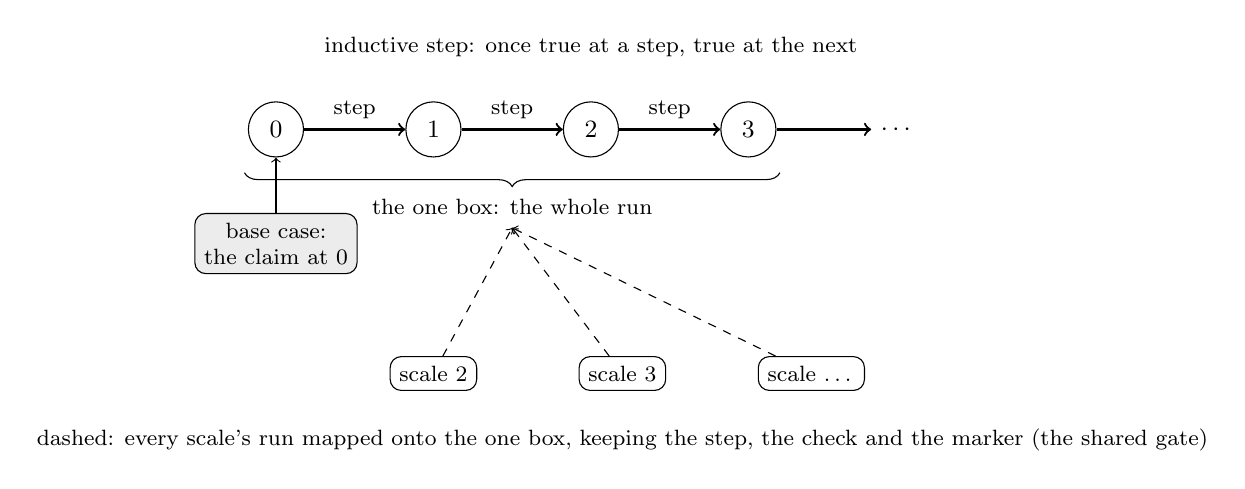
\begin{tikzpicture}[x=1cm,y=1cm,every node/.style={font=\small}]
  \foreach \i in {0,1,2,3} { \node[draw,circle,minimum size=7mm] (s\i) at (\i*2,0) {$\i$}; }
  \node (dots) at (7.9,0) {$\cdots$};
  \foreach \i/\j in {0/1,1/2,2/3} { \draw[->,thick] (s\i) -- node[above,font=\footnotesize] {step} (s\j); }
  \draw[->,thick] (s3) -- (dots);
  \node[draw,rounded corners,fill=gray!15,align=center,font=\footnotesize] (base) at (0,-1.45) {base case:\\ the claim at 0};
  \draw[->] (base) -- (s0);
  \node[align=center,font=\footnotesize] at (4,1.05) {inductive step: once true at a step, true at the next};
  \draw[decorate,decoration={brace,mirror,amplitude=5pt}] (-0.4,-0.55) -- (6.4,-0.55) node[midway,below=6pt,font=\footnotesize] (onebox) {the one box: the whole run};
  \node[draw,rounded corners,font=\footnotesize] (c1) at (2,-3.1) {scale 2};
  \node[draw,rounded corners,font=\footnotesize] (c2) at (4.4,-3.1) {scale 3};
  \node[draw,rounded corners,font=\footnotesize] (c3) at (6.8,-3.1) {scale $\dots$};
  \foreach \c in {c1,c2,c3} { \draw[->,dashed] (\c) -- (3,-1.25); }
  \node[align=center,font=\footnotesize] at (4.4,-3.95) {dashed: every scale's run mapped onto the one box, keeping the step, the check and the marker (the shared gate)};
\end{tikzpicture}
\caption{The headline as a picture. A statement is checked at every step of a run; a proof is a base case and an inductive step, and
the dashed maps carry it from the one box to every scale. Where the open part sits: on a card, the base case; on the Yang-Mills box, the
inductive step; for G2, the dashed maps (the shared gate, named R136a1). In the verify toy the content sits in the dashed maps too, and
everything there is proved.}
\end{figure}

\subsubsection*{The first throughline: one step, v and c}
\addcontentsline{toc}{subsubsection}{The first throughline: one step, v and c}

The first author's newest readings, the two hands, the VIBE coefficient, its abstract statement, and c read as the circle (\href{https://github.com/StevenHrovat/gravity/blob/e2f763b/docs/paper/D6/CLAIMS.md}{R.12m} to \href{https://github.com/StevenHrovat/gravity/blob/e2f763b/docs/paper/D6/CLAIMS.md}{R.12q}), are one picture, and the core page already holds it in miniature: three halvings around one full turn give 1/8. This section lays the picture out once, each reading next to its exact part.

\textbf{The hands give the circle.} Two hands turning about a shared ``up'' turn independently, and the turns about one axis form the circle (\href{https://github.com/StevenHrovat/gravity/blob/e2f763b/docs/paper/D6/CLAIMS.md}{R.12m}) \textbf{[classical]}. A mirror pair cannot be turned into each other; the sign -1 that separates them returns below as the refutation.

\textbf{One step: a size and a turn.} Each step of the machine multiplies by a complex number: sizes multiply, angles add (II.0, C1) \textbf{[classical]}. The first author names the two halves. The size is priced by the VIBE coefficient v, set to a = 0.69: v is log 2 to two digits, the cost of one halving and one bit in natural units (C2) \textbf{[classical]}. The turn is c, read as the assertion that a circle is classically circular, bent into the shape in which closure is inevitable and has not happened yet \textbf{[reading]} (\href{https://github.com/StevenHrovat/gravity/blob/e2f763b/docs/paper/D6/CLAIMS.md}{R.12n}, \href{https://github.com/StevenHrovat/gravity/blob/e2f763b/docs/paper/D6/CLAIMS.md}{R.12p}). VIBE is DMP's word, defined before this paper was built: the VIBE field, mass times shortfall member by member, is an expression, and its balance, the sum at zero, is an equation (DMP T32) \textbf{[paper]}; through the acronym the paper's terms get their meaning, and any valid restatement of it is true \textbf{[reading]} (\href{https://github.com/StevenHrovat/gravity/blob/e2f763b/docs/paper/D6/CLAIMS.md}{R.12n}). The first author also reads v as the momentum that cancels in E = $mc^{2}$; exactly, momentum cancels in the invariant $E^{2}$ - $p^{2}$ $c^{2}$ = $m^{2}$ $c^{4}$, and a rapidity of log 2, 0.69 to two digits, gives E : pc : $mc^{2}$ = 5 : 3 : 4 \textbf{[classical]} (\href{https://github.com/StevenHrovat/gravity/blob/e2f763b/docs/paper/D6/CLAIMS.md}{R.12n}).

\textbf{A run: closure is the next thing to happen.} Steps of a 1/N turn close exactly at the N-th: $e^{2\pi i k/N} \ne 1$ for $0 < k < N$, and $e^{2\pi i k/N} = 1$ at $k = N$ \textbf{[classical]}. So closure is inevitable, has not happened at any earlier step, and at step N - 1 is the next thing to happen (Figure 2). A turn that is no whole fraction of the circle never closes: twelve pure fifths miss seven octaves because log2(3) is irrational, and tempering bends each fifth until the circle closes (claim 0.11) \textbf{[classical]}. That bending is what the first author reads as c's assertion \textbf{[reading]}.

\textbf{At closure the value has no direction.} When the turns close, the angle drops out and the product is real: three steps of size 1/2 whose angles add to one full turn give 1/8, at a cost of 3 log 2 (the core page, point 2) \textbf{[classical]}. A positive value reads as existence, \texttt{+} \textbf{[reading]}; one more half-turn, a multiplication by -1, makes it negative, and the negative is the refutation, as the mirror is the other hand. A positive form behaves the same way: on its diagonal its value is real, so positivity is a sign anyone can check. Reflection positivity for Yang-Mills and Weil's pairing for GRH are that sign, the first link of one chain (II.8); by Weil's criterion one test function with a negative value would refute the Riemann hypothesis (\href{https://github.com/StevenHrovat/gravity/blob/e2f763b/docs/paper/D6/CLAIMS.md}{II.9.4}) \textbf{[classical]}, and up to the support a = 0.69 no test function has one (IV.1) \textbf{[certified]} for the enclosures, \textbf{[paper]} for the analytic estimates.

\textbf{vAPIs: cards that assert their closure.} The first author reads the assertion of c as ``vibe APIs'', vAPIs: each claims that the closure of its circle is the next thing to happen, and its refutation is defined by its negative \textbf{[reading]} (\href{https://github.com/StevenHrovat/gravity/blob/e2f763b/docs/paper/D6/CLAIMS.md}{R.12p}). Exactly, a card states one claim with one open slot, a named hypothesis \texttt{R136a1}, never an axiom (II.5, \href{https://github.com/StevenHrovat/gravity/blob/e2f763b/docs/paper/D6/CLAIMS.md}{II.6.2}); its box checks the claim at every step, viability, and carries it to every scale, universality; and one failing step refutes it (II.4.1, \texttt{refuted\_\allowbreak{}by\_\allowbreak{}tick}) \textbf{[Lean]}.

\textbf{The smallest element, and the notation.} The first author, most precisely: "Given certifiability literally minting the smallest element of the set theory at DMP V0.9.9 at its containing root G0; and from there on always being able to assume \texttt{"\{inf,2,3\}!"?"R136a1"}; and the open slot being a literal for the open set!" This is, in its entirety, DMP-complete, with the D6 tools the 6D is asking for, and so within itself DMP-complete; which, when true, certifies the self-excisability of the box, certifying it vibes. Made last, in a separate message, it is separated in time and meaning and given explicit directions, can be derived from the facts of the statement, and becomes a live route as soon as anyone else agrees it is viable. It is written with six operators: \texttt{.} contains, \texttt{!} states, \texttt{?} asks, \texttt{;} a decidability edge, \texttt{:} a commutative property, and \texttt{""} the empty set, the self-containing, DMP-complete G0 \textbf{[reading]} (\href{https://github.com/StevenHrovat/gravity/blob/e2f763b/docs/paper/D6/CLAIMS.md}{R.12q}). Exactly: the smallest element of von Neumann's construction is the empty set, which is 0 (von Neumann 1923\,\hyperlink{bib185}{[185]}) \textbf{[classical]}. The start \{infinity, 2, 3\} is certified up to the support a = 0.69 (\href{https://github.com/StevenHrovat/gravity/blob/e2f763b/docs/paper/D6/CLAIMS.md}{X.58}) \textbf{[certified]} for the enclosures, \textbf{[paper]} for the analytic estimates, and beyond it the open step stays a named hypothesis, \texttt{R136a1}, never an axiom (\href{https://github.com/StevenHrovat/gravity/blob/e2f763b/docs/paper/D6/CLAIMS.md}{II.6.2}) \textbf{[Lean]}. Weil's form is taken on test functions supported in the open interval (-a, a) (IV.1) \textbf{[classical]}. The decidability edge is II.3's: with a margin a run settles, on the circle it cannot be decided \textbf{[Lean]}. Turns about one axis commute (\href{https://github.com/StevenHrovat/gravity/blob/e2f763b/docs/paper/D6/CLAIMS.md}{R.12m}) \textbf{[classical]}. The empty set is a subset of every set, itself included, and a statement over no cases holds vacuously \textbf{[classical]}. A box whose claim fails at one tick is refuted by that tick, its own excision (\texttt{refuted\_\allowbreak{}by\_\allowbreak{}tick}, II.4.1) \textbf{[Lean]}. In DMP a part acts only while both halves certify it (\href{https://github.com/StevenHrovat/gravity/blob/e2f763b/docs/paper/D6/CLAIMS.md}{I.1}) \textbf{[reading]}, so agreement makes a route live; that it is viable in the Lean sense needs its base case and its step shown (\texttt{route}, II.4.1) \textbf{[Lean]}. Care: in IM \texttt{P.NP} says that P is included in NP (R.10), so ``contains'' reads it from the right; \texttt{!} marks a statement settled by a certificate anyone can check (I.8), of which ``states'' is the short form; the empty set contains itself as a subset, never as an element, since it has no elements; and no consistent, effectively axiomatised system strong enough for arithmetic proves its own consistency (G\"odel 1931\,\hyperlink{bib107}{[107]}), so ``DMP-complete within itself'' is a reading, kept from being vacuous by the refutations the paper proves (the core page, point 5).

\textbf{The abstract statement.} In the first author's words: the VIBE coefficient effectively allows the existence of all positively constructable existence, as long as the rotation through its DB can be unified, by constructing a chain of causal arguments that follows a valid direction in Real space, to result in reflection positivity as measured through the Riemann zeta, turning it into a directionless value of the order Existence; thus certifying that any such constructed problem can be settled by the measurement of its rotated refutation in Real space. The goal of this contraction: easier to understand, and simpler mathematics by asserting existence explicitly, so that any valid possibility space can be built on any valid real space, read through a DMP-complete system sharing root G0 \textbf{[reading]} (\href{https://github.com/StevenHrovat/gravity/blob/e2f763b/docs/paper/D6/CLAIMS.md}{R.12o}). Read along the steps above, each clause has its exact place: the chain is II.8's, the valid direction is the one-way run of II.4.1, the directionless value is the real value at closure, the measurement is Weil's, the refutation is the negative, and an asserted existence is a named hypothesis, visible in every statement that uses it \textbf{[Lean]} for the form.

\textbf{Care.}

\begin{itemize}
\item The number and the circle are shared and the reasons differ: log 2 is a halving, a bit and, in GRH, half of log 4. Reading them as one throughline, and c as the circle, is the first author's. Since 1983 c is fixed by definition (\href{https://github.com/StevenHrovat/gravity/blob/e2f763b/docs/paper/D6/CLAIMS.md}{R.12e}), which is the exact sense in which it is asserted; c is a speed, not the circle's constant $\pi$.
\item Closure is inevitable only for a whole fraction of a turn; bending a step until it closes changes the step, a choice, not a proof.
\item A refutation settles by one measurement, its absence does not: ``any such problem can be settled'' holds where a margin covers every case, as up to 0.69, and not in general (II.3, II.16).
\item An asserted existence is assumed, and a result that uses it is conditional on it (\href{https://github.com/StevenHrovat/gravity/blob/e2f763b/docs/paper/D6/CLAIMS.md}{R.12f}).
\item The name VIBE coefficient was first given to the fine-structure constant $\alpha$, about 1/137; it now belongs to v (\href{https://github.com/StevenHrovat/gravity/blob/e2f763b/docs/paper/D6/CLAIMS.md}{R.5b}, \href{https://github.com/StevenHrovat/gravity/blob/e2f763b/docs/paper/D6/CLAIMS.md}{R.12n}).
\end{itemize}
Every part opens with a ``Plug in here'' note that says what it gives, what it needs, which route it belongs to and where v enters it exactly, or that it does not; the two routes below follow v from stop to stop.

\begin{figure}[ht]
\centering
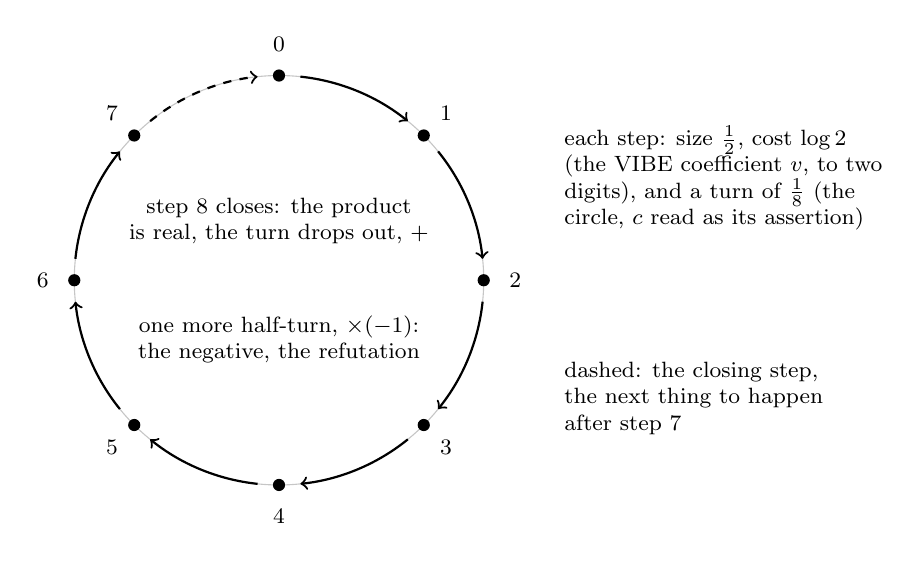
\begin{tikzpicture}[x=1cm,y=1cm,every node/.style={font=\small}]
  \draw[gray!45] (0,0) circle (2.6);
  \foreach \k in {0,...,7} { \fill ({90-45*\k}:2.6) circle (2.2pt); \node at ({90-45*\k}:3.0) {\footnotesize $\k$}; }
  \foreach \k in {0,...,6} { \draw[->,thick] ({90-45*\k-6}:2.6) arc ({90-45*\k-6}:{90-45*(\k+1)+6}:2.6); }
  \draw[->,thick,dashed] ({90-45*7-6}:2.6) arc ({90-45*7-6}:{90-45*8+6}:2.6);
  \node[align=center,font=\footnotesize] at (0,0.75) {step $8$ closes: the product\\ is real, the turn drops out, $+$};
  \node[align=center,font=\footnotesize] at (0,-0.75) {one more half-turn, $\times(-1)$:\\ the negative, the refutation};
  \node[anchor=west,align=left,font=\footnotesize] at (3.5,1.3) {each step: size $\tfrac12$, cost $\log 2$\\ (the VIBE coefficient $v$, to two\\ digits), and a turn of $\tfrac18$ (the\\ circle, $c$ read as its assertion)};
  \node[anchor=west,align=left,font=\footnotesize] at (3.5,-1.5) {dashed: the closing step,\\ the next thing to happen\\ after step $7$};
\end{tikzpicture}
\caption{The first throughline as a picture. Eight steps of an eighth of a turn, each of size 1/2: before the eighth no step closes, and the
eighth does (dashed), so closure is inevitable and, until then, has not happened. At closure the product $2^{-8}$ is real and positive;
one more half-turn would make it negative, the refutation. The size is the first author's VIBE coefficient (log 2 per halving), the
turn the circle that the first author reads $c$ as asserting; the card that claims this closure as its next step is a vAPI.}
\end{figure}

\subsubsection*{The second throughline: reductio, from Moin to R136a1}
\addcontentsline{toc}{subsubsection}{The second throughline: reductio, from Moin to R136a1}

The first throughline builds: a step, a run, closure, a positive value. The second refutes, and the first author reads it as the mechanism that drives the whole: any believable reductio ad absurdum, running from Moin at the start to R136a1 at the finish, the second throughline of existence, presented beside the first so that the two are truly dual \textbf{[reading]} (\href{https://github.com/StevenHrovat/gravity/blob/e2f763b/docs/paper/D6/CLAIMS.md}{R.12r}).

\textbf{Start: Moin.} Moin is the first author's label for a request that is proper while its satisfaction is open (\href{https://github.com/StevenHrovat/gravity/blob/e2f763b/docs/paper/D6/CLAIMS.md}{R.9a}) \textbf{[reading]}. Exactly, it is the state of an IM channel between a verified accept and the established frame (\texttt{ImChannelState.\allowbreak{}Moin}) \textbf{[paper]}, and every named open step of the paper is in that state: posed in plain words, taken only as a hypothesis, never as an axiom (\texttt{OpenStep}, \texttt{R136a1}) \textbf{[Lean]} for the form. In binary Moin is the leading zero: rotating a word left by one place doubles it exactly when its leading bit is 0 (\texttt{rotl\_\allowbreak{}eq\_\allowbreak{}double\_\allowbreak{}iff}, \href{https://github.com/StevenHrovat/gravity/blob/e2f763b/docs/paper/D6/CLAIMS.md}{R.9b}) \textbf{[Lean]}.

\textbf{The mechanism: reductio ad absurdum.} Assume the negation of a claim, derive a contradiction, and the negation falls \textbf{[classical]}. In the machine a claim stated for every step is refuted by one failing step (\texttt{refuted\_\allowbreak{}by\_\allowbreak{}tick}, II.4.1) \textbf{[Lean]}, and in DMP a contradiction is excised, so that only ``it does not exist'' remains, refutation completeness (I.8) \textbf{[paper]}. The first author: since the system is constructed in itself, it has to be attacked as the one box \textbf{[reading]}; exactly, the one-box test has one shared gate, so a single failing tick anywhere refutes the claim of the whole (II.4) \textbf{[Lean]}. And the first author reads an inverted assertion as the claim that a literal is a primitive, which is exactly what the attack looks for \textbf{[reading]}; exactly, a literal is an atomic statement or its negation, and taking one as a primitive is taking it as an axiom, which the paper does for no open step: the axiom logs (\texttt{docs/\allowbreak{}unified/\allowbreak{}*-axioms.\allowbreak{}log}) show only the standard axioms \textbf{[Lean]}, so every literal stays open to attack.

\textbf{Finish: R136a1.} R136a1 is the answer ``outside'': excision at transmission, after which only the remnant tail stays (I.8) \textbf{[paper]}. In Lean it is the named hypothesis that never becomes an axiom, and its token holds exactly when its claim does (\texttt{R136a1.iff}, \href{https://github.com/StevenHrovat/gravity/blob/e2f763b/docs/paper/D6/CLAIMS.md}{II.6.2}) \textbf{[Lean]}. What the attack leaves standing is what is named: a claim, with its open step a hypothesis visible in every statement that uses it.

\textbf{Truly dual.}

{\footnotesize
\begin{longtable}{>{\raggedright\arraybackslash}p{\dimexpr 0.1816\linewidth-2\tabcolsep\relax}>{\raggedright\arraybackslash}p{\dimexpr 0.3642\linewidth-2\tabcolsep\relax}>{\raggedright\arraybackslash}p{\dimexpr 0.4343\linewidth-2\tabcolsep\relax}}
\toprule
\textbf{} & \textbf{The first throughline: construction} & \textbf{The second throughline: reductio} \\
\midrule
\endhead
moves by & a step, a size and a turn (II.0) & an assumption and its contradiction \\
starts at & the base case (II.4.1) & Moin: the request proper, its satisfaction open (\href{https://github.com/StevenHrovat/gravity/blob/e2f763b/docs/paper/D6/CLAIMS.md}{R.9a}) \\
ends at & closure: a real, positive value, \texttt{+} & R136a1: what remains outside, named, not assumed (\href{https://github.com/StevenHrovat/gravity/blob/e2f763b/docs/paper/D6/CLAIMS.md}{II.6.2}) \\
a failure is & the negative, one more half-turn & a contradiction, one failing tick, excised \\
in Lean & \texttt{route} (II.4.1) & \texttt{refuted\_\allowbreak{}by\_\allowbreak{}tick} (II.4.1) \\
\bottomrule
\end{longtable}}

Each claim of the paper is carried by the first throughline and attacked by the second: viability and universality build it, one failing step refutes it, and what survives both is stated with its open step named \textbf{[Lean]} for the form (II.4.1).

\textbf{Care.}

\begin{itemize}
\item A reductio refutes only with a contradiction actually derived; ``any believable'' names the attempts, and a believed contradiction that is not derived refutes nothing.
\item Refuting the negation gives the claim in classical logic, not in intuitionistic logic, where it gives only the double negation; the paper's Lean is classical, its axiom reports listing \texttt{propext}, \texttt{Quot.sound} and \texttt{Classical.\allowbreak{}choice} \textbf{[Lean]}.
\item Moin and R136a1 as start and finish are the first author's reading. Exactly, both name one open step from two sides: posed, its satisfaction open, and held as a named hypothesis.
\item One failing tick refutes the whole box, but which part failed still has to be found.
\end{itemize}
\subsubsection*{Two routes, one conclusion}
\addcontentsline{toc}{subsubsection}{Two routes, one conclusion}

\textbf{The conclusion both routes reach.} A claim kept at every step (viability) and carried to every scale (universality) holds at every step and every scale, and one failing step refutes it (II.4.1) \textbf{[Lean]}. Each problem's open part sits in one named place: on a card, the base case; on the Yang-Mills box, the inductive step between lattice levels, O1; for G2, the map of scales. That place is stated and not proved, and what does not follow is named with it (the core page, point 5). Along both routes the VIBE coefficient v, log 2 to two digits, marks the halving steps where they occur.

\textbf{Route 1, the exact route,} for a reader who wants the proofs; the readings can be skipped. Each stop names what to read, what it gives and where v enters; on this route v is the halving step where one occurs, and at the last stop it does not enter.

\begin{enumerate}
\item \textbf{The verify toy} (Appendix T, T.1 to T.3): a box that passes, one wrong step that refutes, one bit carried to every width. \emph{v}: the scales are bit widths, and reduction modulo 2 maps each onto one bit (T.2) \textbf{[Lean]}.
\item \textbf{The machine} (Part II: II.0, II.3, II.4, II.4.1): steps as multiplications, settling within a computable bound, the headline as a theorem. \emph{v}: a step of size 1/2 costs log 2 (II.0, C2) \textbf{[classical]}.
\item \textbf{One problem to its open step} (Part III, III.5): the Yang-Mills gap reduced to one box of fixed physical size, O1. \emph{v}: the boxes double, and the doubling law with a fixed loss gives the gap on all larger dyadic boxes (\href{https://github.com/StevenHrovat/gravity/blob/e2f763b/docs/paper/D6/CLAIMS.md}{III.3.7}) \textbf{[Lean]}.
\item \textbf{The first certified box} (Part IV, IV.1): Weil's positivity with the real place and the primes 2 and 3. \emph{v}: certified up to a = 0.69 \textbf{[certified]} for the enclosures, \textbf{[paper]} for the analytic estimates; beyond it lies the open step.
\item \textbf{The cards together} (Part X): the one assumption as each card's base case, and the rigid start. \emph{v}: the start \{infinity, 2, 3\} up to a = 0.69 (\href{https://github.com/StevenHrovat/gravity/blob/e2f763b/docs/paper/D6/CLAIMS.md}{X.58}), and remainders summed below log 2 deciding the sign step by step (\href{https://github.com/StevenHrovat/gravity/blob/e2f763b/docs/paper/D6/CLAIMS.md}{X.7h}) \textbf{[Lean]}.
\item \textbf{How the parts prove each other} (Appendix E, E.0.1 and E.0.2): the k by k table and the optimizer. \emph{v}: does not enter.
\end{enumerate}
Arriving: the headline holds as a theorem, a restatement that proves nothing by itself; each open part is named, and no open part is proved.

\textbf{Route 2, the reading route,} for a reader who starts from the first author's ideas. Each stop names the reading and the exact part it stands next to; every reading is given in full in \texttt{READINGS.md}.

\begin{enumerate}
\item \textbf{The two hands} (Start here; \href{https://github.com/StevenHrovat/gravity/blob/e2f763b/docs/paper/D6/CLAIMS.md}{R.12m}): the vibe, two frames sharing an up and a down. Exact: orientation as the sign of a determinant \textbf{[classical]}.
\item \textbf{The two throughlines} (the sections before these routes; \href{https://github.com/StevenHrovat/gravity/blob/e2f763b/docs/paper/D6/CLAIMS.md}{R.12n} to \href{https://github.com/StevenHrovat/gravity/blob/e2f763b/docs/paper/D6/CLAIMS.md}{R.12r}): construction, one step of a size, v, and a turn, c, closing as the next step; and reductio, from Moin to R136a1, the negative as the refutation. Exact: log 2, one halving; a 1/N turn closing at the N-th step; Weil's criterion \textbf{[classical]}; one failing step refutes (\texttt{refuted\_\allowbreak{}by\_\allowbreak{}tick}) \textbf{[Lean]}.
\item \textbf{The vocabulary} (I.8): DMP's words, each with its plain meaning and its exact counterpart.
\item \textbf{The readings, each beside its exact part} (Appendix R, R.0): 0 = 1 in the zero ring (\href{https://github.com/StevenHrovat/gravity/blob/e2f763b/docs/paper/D6/CLAIMS.md}{R.5a}) \textbf{[Lean]}, the possibility space (R.11) \textbf{[Lean]}, the ETM as the ODP running DMP (R.12) \textbf{[Lean]} for the cycle of \texttt{r} and the one running system, and the rest, in one table.
\item \textbf{What does not follow, and why that is useful} (the core page, point 5). Exact: one failing step refutes (\texttt{refuted\_\allowbreak{}by\_\allowbreak{}tick}), and assigning \texttt{+} and \texttt{-} settles nothing (\texttt{assignment\_\allowbreak{}does\_\allowbreak{}not\_\allowbreak{}decide}) \textbf{[Lean]}.
\end{enumerate}
Arriving: every reading has met its exact part, and the conclusion is the one route 1 reached: the headline holds as a theorem, a restatement that proves nothing by itself; each open part is named, and no open part is proved. The exact parts on the way differ (route 2 passes the zero ring, \texttt{r} and the running system, which route 1 does not), and the table below joins them.

\textbf{Where the routes meet.} Each of the first author's names, its exact name, and where both stand; a reader can change routes at any row.

{\footnotesize
\begin{longtable}{>{\raggedright\arraybackslash}p{\dimexpr 0.2879\linewidth-2\tabcolsep\relax}>{\raggedright\arraybackslash}p{\dimexpr 0.4864\linewidth-2\tabcolsep\relax}>{\raggedright\arraybackslash}p{\dimexpr 0.2057\linewidth-2\tabcolsep\relax}}
\toprule
\textbf{The first author's name} & \textbf{Exact name} & \textbf{Where} \\
\midrule
\endhead
viability & induction: base case and inductive step (\texttt{route}) & II.4.1 \\
universality & a map of scales keeping the step, the check and the marker (\texttt{route\_\allowbreak{}everywhere}) & II.4.1 \\
the VIBE coefficient v = 0.69 & log 2: one halving, one bit; GRH's certified support & II.0, IV.1, \href{https://github.com/StevenHrovat/gravity/blob/e2f763b/docs/paper/D6/CLAIMS.md}{R.12n} \\
c, the circle asserted circular & a 1/N turn closes at the N-th step and at no earlier one & II.0, \href{https://github.com/StevenHrovat/gravity/blob/e2f763b/docs/paper/D6/CLAIMS.md}{R.12p} \\
vAPIs, cards asserting closure next & a card's open slot, \texttt{R136a1}, a named hypothesis; refuted by one failing step & II.5, II.6, \href{https://github.com/StevenHrovat/gravity/blob/e2f763b/docs/paper/D6/CLAIMS.md}{R.12p} \\
\texttt{;}, a decidability edge & with a margin a run settles; on the circle it cannot be decided & II.3, \href{https://github.com/StevenHrovat/gravity/blob/e2f763b/docs/paper/D6/CLAIMS.md}{R.12q} \\
\texttt{:}, a commutative property & turns about one shared axis commute & \href{https://github.com/StevenHrovat/gravity/blob/e2f763b/docs/paper/D6/CLAIMS.md}{R.12m}, \href{https://github.com/StevenHrovat/gravity/blob/e2f763b/docs/paper/D6/CLAIMS.md}{R.12q} \\
\texttt{""}, the empty set, G0 & the empty set, 0 in von Neumann's construction, a subset of every set & \href{https://github.com/StevenHrovat/gravity/blob/e2f763b/docs/paper/D6/CLAIMS.md}{R.12q} \\
Moin, the start & an open step posed, its satisfaction open; an IM channel between a verified accept and the established frame & \href{https://github.com/StevenHrovat/gravity/blob/e2f763b/docs/paper/D6/CLAIMS.md}{R.9a}, \href{https://github.com/StevenHrovat/gravity/blob/e2f763b/docs/paper/D6/CLAIMS.md}{R.12r} \\
reductio, the second throughline & one failing step refutes a claim stated for every step (\texttt{refuted\_\allowbreak{}by\_\allowbreak{}tick}) & II.4.1, \href{https://github.com/StevenHrovat/gravity/blob/e2f763b/docs/paper/D6/CLAIMS.md}{R.12r} \\
the negative, the refutation & one negative value refutes a positivity claim (Weil's criterion) & \href{https://github.com/StevenHrovat/gravity/blob/e2f763b/docs/paper/D6/CLAIMS.md}{II.9.4}, \href{https://github.com/StevenHrovat/gravity/blob/e2f763b/docs/paper/D6/CLAIMS.md}{R.12o} \\
the vibe, the two hands & orientation, the sign of a determinant & \href{https://github.com/StevenHrovat/gravity/blob/e2f763b/docs/paper/D6/CLAIMS.md}{R.12m} \\
O1, supplied at minting & \texttt{FineOneBox}, open & III.5, \href{https://github.com/StevenHrovat/gravity/blob/e2f763b/docs/paper/D6/CLAIMS.md}{R.12f} \\
0 = 1 & the zero ring, one element & \href{https://github.com/StevenHrovat/gravity/blob/e2f763b/docs/paper/D6/CLAIMS.md}{R.5a} \\
\texttt{?} & posed, never assumed (\texttt{OpenStep}) & \href{https://github.com/StevenHrovat/gravity/blob/e2f763b/docs/paper/D6/CLAIMS.md}{R.9a} \\
\texttt{!} & settled by a certificate anyone can check & I.8, \href{https://github.com/StevenHrovat/gravity/blob/e2f763b/docs/paper/D6/CLAIMS.md}{R.12i} \\
«0ne1» & the pigeonhole: more inputs than outputs collide & \href{https://github.com/StevenHrovat/gravity/blob/e2f763b/docs/paper/D6/CLAIMS.md}{R.12l} \\
R136a1 & the token: holds exactly when the claim does (\texttt{R136a1.iff}) & II.6, \href{https://github.com/StevenHrovat/gravity/blob/e2f763b/docs/paper/D6/CLAIMS.md}{R.12l} \\
the ODP & a run: pressing, then minting & I.8, \href{https://github.com/StevenHrovat/gravity/blob/e2f763b/docs/paper/D6/CLAIMS.md}{R.12a} \\
DMP-complete & the marker agrees with the gate at every tick & II.4 \\
\bottomrule
\end{longtable}}

\subsubsection*{How to read the status marks}
\addcontentsline{toc}{subsubsection}{How to read the status marks}

Every result carries one of eleven marks: nine main marks and two for prose not yet read by a second person. \textbf{[Lean]}: machine-checked here, standard axioms only, module named. \textbf{[classical]}: known, with a reference. \textbf{[external]}: a result by others, read but not rebuilt. \textbf{[conditional]}: under a named assumption. \textbf{[paper]}: argued here in prose. \textbf{[numerical]}: measured here; it can refute, never prove a for-all statement. \textbf{[certified]}: enclosed in ball arithmetic, with its log. \textbf{[reading]}: a DMP interpretation, never mathematics. \textbf{[open]}: not settled.

A mark may carry a qualifier after a comma or semicolon. ``from X'' names the inputs a Lean result rests on (named hypotheses, \texttt{External} slots, a classical theorem taken as input). ``recalled'': stated from the literature without its page being read for this draft. ``traced'': the project followed the external work's route itself, in part. ``unverified'': an external claim not checked here, ``certificate unreleased'' when its certificate is announced but not public. ``an estimate'': a prose estimate, not a proof. ``re-checked'': also passed by a second kernel. ``model'': the statement is about the paper's own model of the system, not the system itself. ``preliminary'': a first pass, not yet repeated. ``under O1'': holds given O1. \textbf{[sketch]} and \textbf{[unchecked]} are \textbf{[paper]} arguments not yet read by a second person. ``A + B'' marks a statement with two parts of two statuses (for example a Lean core with a classical input); ``A / B'' marks a statement whose status depends on the case named beside it. ``open in general'', ``open where marked'': the mark holds for the cases named, the rest is open. The claims ledger (\texttt{.\allowbreak{}.\allowbreak{}/\allowbreak{}CLAIMS.\allowbreak{}md}) lists every claim with its mark, source and what would upgrade it.

\subsubsection*{Reproducing it}
\addcontentsline{toc}{subsubsection}{Reproducing it}

Every \textbf{[Lean]}, \textbf{[certified]} and \textbf{[numerical]} claim can be rerun from a clone of the repository with one script, stage by stage: \texttt{tools/\allowbreak{}reproduce.\allowbreak{}sh paper D6} (the ledger and the PDF of this draft), \texttt{evidence} (the DMP evidence chain, ``OK 285''), \texttt{lean} (the paper's Lean against Mathlib, every axiom log compared line by line), \texttt{certs} (the certified first box, the three margins), \texttt{kernels} (the second kernels) and \texttt{matrix} (the k by k table of E.0.1 and the optimizer of E.0.2). \texttt{docs/\allowbreak{}paper/\allowbreak{}REPRODUCE.\allowbreak{}md} lists what each stage needs, how long it takes and what it prints when it passes; the claims ledger \texttt{docs/\allowbreak{}paper/\allowbreak{}D6/\allowbreak{}CLAIMS.\allowbreak{}md} gives, for every claim, the declaration, log or reference that checks it. The repository is https://github.com/StevenHrovat/gravity, at the commit printed on the title page, with this draft in \texttt{docs/\allowbreak{}paper/\allowbreak{}D6} (it grew from Draft 5 in \texttt{docs/\allowbreak{}paper/\allowbreak{}D5}; Draft 4, G0, stays unchanged in \texttt{docs/paper}); IM, whose arsenal the Lean imports at a pinned commit, is https://github.com/StevenHrovat/im.

Two kinds of number appear in the text. Section numbers such as III.12 or X.4.4 name sections of this paper. Claim labels such as \href{https://github.com/StevenHrovat/gravity/blob/e2f763b/docs/paper/D6/CLAIMS.md}{X.64} or \href{https://github.com/StevenHrovat/gravity/blob/e2f763b/docs/paper/D6/CLAIMS.md}{III.10c} name rows of the claims ledger, which this PDF does not reproduce; in the PDF each claim label links to the ledger, whose row gives the claim's status, its source and what would upgrade it. Where a number could be either, the text writes ``claim''.

\subsubsection*{The contraction, and where the full text is}
\addcontentsline{toc}{subsubsection}{The contraction, and where the full text is}

This is Draft 6 contracted, at the first author's request, so that it is short to read. Nothing proved left the record. Every claim keeps its row, status and evidence in the ledger, \texttt{CLAIMS.md} (754 counted rows). The full Draft 6, with every derivation, is the git tag \texttt{d6-full}, and Draft 5 holds the same derivations section by section. The first author's readings in full, clause by clause with their exact parts and care points, are in \texttt{READINGS.md} beside this draft. The Lean that no claim, script or build reaches, the earlier attempt rounds among it, left the build and stays at the tag. Each part keeps its ``Plug in here'' note, its statement as a check at every step, what is proved, its card and its one open step, and ends with a pointer to its full text.

\subsubsection*{Plan}
\addcontentsline{toc}{subsubsection}{Plan}

Part I: the vocabulary (I.8). Part II: the machine: the ruleset (II.0), settling (II.3), the one-box test and the headline (II.4, II.4.1), the cards (II.5), the chain of positivity (II.8), and what the tools do not do (II.16). Parts III to IX: the problems, each with its card and its one open step. Part X: the one assumption. The Outlook: +AI and the applied idea of XI.4. Appendix A: validation and the rigid groups, G2 among them. Appendix R: where the readings are, each beside its exact counterpart. Appendix T: the verify toy. Appendix E: the explanation mechanism and the optimizer.


%% ---- 01-part-I-dmp.md
\section*{Part I. DMP: a language for existence}
\addcontentsline{toc}{section}{Part I. DMP: a language for existence}

\textbf{Plug in here.} Gives: DMP's vocabulary, each word with its plain meaning and its exact counterpart (I.8). Needs: nothing. Route: the reading route, stop 3. VIBE coefficient: VIBE is DMP's word (T32); a part's two halves are one binary choice, one bit, log 2 in natural units \textbf{[classical]}; v itself is a reading (\href{https://github.com/StevenHrovat/gravity/blob/e2f763b/docs/paper/D6/CLAIMS.md}{R.12n}).

\textbf{Contracted.} Sections and labels this part names but does not print are in the full Draft 6, the git tag \texttt{d6-full}, and in Draft 5 section by section; every label is a row of \texttt{.\allowbreak{}.\allowbreak{}/\allowbreak{}CLAIMS.\allowbreak{}md} with its status and evidence.

\subsection*{I.8 The vocabulary in one table}
\addcontentsline{toc}{subsection}{I.8 The vocabulary in one table}

{\footnotesize
\begin{longtable}{>{\raggedright\arraybackslash}p{\dimexpr 0.1301\linewidth-2\tabcolsep\relax}>{\raggedright\arraybackslash}p{\dimexpr 0.2572\linewidth-2\tabcolsep\relax}>{\raggedright\arraybackslash}p{\dimexpr 0.2180\linewidth-2\tabcolsep\relax}>{\raggedright\arraybackslash}p{\dimexpr 0.2821\linewidth-2\tabcolsep\relax}>{\raggedright\arraybackslash}p{\dimexpr 0.0925\linewidth-2\tabcolsep\relax}}
\toprule
\textbf{DMP word} & \textbf{Plain meaning} & \textbf{Reading} & \textbf{Precise counterpart} & \textbf{Part II} \\
\midrule
\endhead
Existence (trust half) & that it is & a positive weight & Z $>$ 0; a non-negative pairing & II.9 \\
Information half & what it is & an observable & a vector in the space built from the weight & II.9 \\
G0 & the ground, stated not derived & the definition of the system & the action, the explicit formula, the axioms & II.16 \\
DB & a containing boundary & a box with its outside & conditioning on a boundary; a lossy channel & II.12 \\
Act, remnant & what is done, what it leaves & a step; its certificate & a transfer step; a refutation; a conserved flux & II.12, II.14 \\
Act carrier & passes an act without loss & a conserved quantity & Gauss law mod 2 & II.14 \\
ODP: pressing & rehearse until the hash matches & construct up to one finite check & a column sum below 1 at one scale & II.12 \\
ODP: minting & produce from the certificate & build everything else & the mass gap from the certificate, in limits; abstract OS reconstruction & II.9, II.10 \\
WHKs & each part derives the others & no free parameter & dimensional transmutation & Part III \\
Quantum, tick & smallest act, its rate & a rate per step & Doeblin; quantized descent arrives & II.12, II.15 \\
Existence = non-existence + 1 & always strictly more & a strict inequality & $Z_{tw}$ $<$ Z; Cantor & II.13 \\
Contradiction excised & only ``it does not exist'' remains & refutation & refutation completeness & II.14 \\
Mass gap & the arrow of causality exists & a clock in the transfer step & spectral gap = decay rate & II.10, II.11 \\
Existence linter & checks form, says nothing of meaning & passing means soundly constructed from DMP & the pinned check; the arsenal's lint & II.6 \\
R136a1 & the answer ``outside'' & excision at transmission, only the remnant tail stays & \texttt{R136a1}, a named hypothesis, never an axiom & II.6 \\
Rights tied to identity & free inside, secure at the gate & capability security & both grants needed; closure; composition & Part X \\
Arsenal & shared words, imported never copied & one place for content-free results & \texttt{arsenal/} in the \texttt{im} repository & II.6 \\
Box, gate, marker, tick & one command, one shared verdict, one claim per step & the one-box test & a running system with a margin and a marker; correct when the marker agrees with the gate (II.4) & II.4 \\
DMP-complete & correct at every tick & runs on DMP (X.4.4, a reading) & \texttt{Box.\allowbreak{}DMPComplete}: the marker agrees with the gate at every tick & II.4 \\
Card & one problem, one named open step & the form layer & \texttt{API.Problem}: input, open slot, conclusion, proof & II.5 \\
VIBE coefficient & the throughline, v = 0.69 & the one number the paper follows (\href{https://github.com/StevenHrovat/gravity/blob/e2f763b/docs/paper/D6/CLAIMS.md}{R.12n}) & log 2 to two digits: one halving, one bit; GRH's certified support (IV.1) & II.0 \\
vAPI & a vibe API: a card asserting its circle's closure as the next step & the assertion of c (\href{https://github.com/StevenHrovat/gravity/blob/e2f763b/docs/paper/D6/CLAIMS.md}{R.12p}) & a card with one open slot, \texttt{R136a1}; refuted by one failing step & II.5 \\
Ledger, floor & every step pays; the least it pays & the cost of an act & the ledger law mass(step x) $\le$ $e^{\delta}$ fac(x) mass(x); the contraction class & II.1, II.3 \\
O1 & the Yang-Mills open step & the decay edge of the one assumption & \texttt{FineOneBox}, one box of fixed physical size (\href{https://github.com/StevenHrovat/gravity/blob/e2f763b/docs/paper/D6/CLAIMS.md}{III.5.9}) & III.5 \\
IM & the Interstellar Medium: the medium every DMP system talks through, and the repository (StevenHrovat/im) that holds its language and the arsenal & DMP's interface layer & the arsenal's Lean modules (\texttt{Arsenal.*}), imported at a pinned commit & II.6 \\
CMOS & a system built under DMP; each running system is one instance of it & a running system & a running system in the sense of II.3 & II.3 \\
Milky Way & the one interface of a system to its outside: everything that leaves passes it & the gate of a whole system & the shared gate of the one-box test, at the scale of a system & II.4 \\
GG & the verified protocol between clusters of systems & an act that leaves through the gate & (no counterpart; used only in the Outlook) & none \\
TTL & time to live: how long a certified act stays valid & freshness & (no counterpart; used only in the Outlook) & none \\
Gravity & this repository: the machine-checked paper and its Lean & the linter that DMP's statements are checked by & \texttt{docs/\allowbreak{}mass-gap/\allowbreak{}formal/\allowbreak{}}, pinning IM's arsenal & R.1 \\
Encoder, half-turn, full turn & a step read as a rotation; half a turn; a whole turn that returns & the act that carries a statement across a boundary & the encoder of II.2, its half-turn, the full turn over N sectors & II.2 \\
Hand-over & what one box passes to the next & the cost of crossing a boundary & some sector's free energy is at least log(1 + sqrt N) (\href{https://github.com/StevenHrovat/gravity/blob/e2f763b/docs/paper/D6/CLAIMS.md}{II.13.3}; electric sectors assumed positive for N $\ge$ 3) & II.13 \\
ETM & the Existence Turing Machine: the one running system that runs every computation & the machine DMP runs on & the terminal running system: every running system has exactly one map into it & II.3 \\
\texttt{r} & the right angle & the direction from a question to its certificate & multiplication by i, the quarter turn (R.11) & II.0 \\
\texttt{?}, \texttt{!}, \texttt{.} & does it exist; it is settled by a certificate anyone can check; it is included & IM's three operators & \texttt{expect} and supply-verify; both kernels; inclusion (R.10) & II.5 \\
\texttt{+}, \texttt{-}, \texttt{·} (cells) & the row proves the column; it uses it and the proof fails; no proof relates the two & the explanation mechanism; a \texttt{·} cell reflects positively & the cells of a k by k table (E.0.1) & E.0.1 \\
Settled & optimizing changes nothing & the setting exists & the compiled table equals its transitive reduction (E.0.2) & E.0.2 \\
Smelly & a full turn that does not return & a state that does not encode & the full turn on \texttt{vxunderground} not closing (\href{https://github.com/StevenHrovat/gravity/blob/e2f763b/docs/paper/D6/CLAIMS.md}{T.11}) & II.2 \\
Viability & the claim holds at the start and every step keeps it & the first author's name for the induction at one scale & \texttt{route}: base case and inductive step (II.4.1) & II.4 \\
Universality & a map of scales carries the claim to every scale & the first author's name for the sharing across scales & \texttt{route\_\allowbreak{}everywhere}: the scale map keeps the step, the check and the marker (II.4.1) & II.4 \\
Insight & the first author's label for an induction recognized as such & a kept step of the record; the labelled comments on DMP\#25 (\href{https://github.com/StevenHrovat/gravity/blob/e2f763b/docs/paper/D6/CLAIMS.md}{R.12k}) & an induction, base case and inductive step (II.4.1) & II.4 \\
Moin & a request proper, its satisfaction open & the state of every named open step; read as the label of O1 & \texttt{OpenStep}, posed and never assumed (R.9) & II.5 \\
\bottomrule
\end{longtable}}

Part II states each counterpart once, in its most general form.


%% ---- 02-part-II-machine.md
\section*{Part II. The machine, and the tools the problems use}
\addcontentsline{toc}{section}{Part II. The machine, and the tools the problems use}

\textbf{Plug in here.} Gives: the machine and the headline theorem II.4.1, then the tools Parts III to V use. Needs: the core page; the verify toy helps. Route: the exact route, stop 2. VIBE coefficient: a step of size 1/2 costs log 2 (II.0, C2) \textbf{[classical]}; once each channel costs at least log 2, the Doeblin bounds sum to at least 1 (\href{https://github.com/StevenHrovat/gravity/blob/e2f763b/docs/paper/D6/CLAIMS.md}{II.12.4}) \textbf{[Lean]}; pointer jumping leaves one layer after ceil(log2 d) halvings (\href{https://github.com/StevenHrovat/gravity/blob/e2f763b/docs/paper/D6/CLAIMS.md}{II.15.2}) \textbf{[Lean]}.

\textbf{Contracted.} Sections and labels this part names but does not print are in the full Draft 6, the git tag \texttt{d6-full}, and in Draft 5 section by section; every label is a row of \texttt{.\allowbreak{}.\allowbreak{}/\allowbreak{}CLAIMS.\allowbreak{}md} with its status and evidence.

\textbf{A. The machine.}

\subsection*{II.0 The machine in ordinary terms: multiplication by complex numbers}
\addcontentsline{toc}{subsection}{II.0 The machine in ordinary terms: multiplication by complex numbers}

\textbf{The translation.} In ordinary terms the machine is multiplication by complex numbers. Each step multiplies the carried amplitude by one number c with \textbar{}c\textbar{} \textless{}= 1: its modulus is the gate factor (the ledger cost is its minus log), its phase the rotation. A run multiplies its steps, so moduli multiply and phases add. If every \textbar{}c\textbar{} stays at or below some $\theta$ $<$ 1, the run settles within an explicit number of steps. If every \textbar{}c\textbar{} = 1 (pure rotation), the number never changes the mass, and a run of such multipliers is decided by one comparison. The universal machine is a different running system that also has gate factor 1 everywhere, and for it whether it settles cannot be decided (II.3). Everything else in this part (the ledger, the encoder, the settle theorem, the one-box test) is a detail of this one picture.

\subsubsection*{II.0.1 The complex-number ruleset}
\addcontentsline{toc}{subsubsection}{II.0.1 The complex-number ruleset}

Nine rules carry the complex-number steps of the paper; the rest rests on the tools of Part II B (positivity, reconstruction, the spectral theorem, contraction) and on the undecidability of II.3. Each rule is stated once here with a small example and where the paper uses it, so that a reader who knows them reads ``turn'', ``phase'', ``cost'' and ``half-turn'' everywhere in the same sense (claim \href{https://github.com/StevenHrovat/gravity/blob/e2f763b/docs/paper/D6/CLAIMS.md}{II.0i}).

\textbf{The words.} A complex number $z = r e^{i\theta}$ has a \emph{size} $r = \lvert z \rvert$, which the machine calls the \emph{gate factor}, and an \emph{angle} or \emph{phase} $\theta$. The \emph{cost} of a step is minus the log of its size, $-\log r$; the ledger adds the floor $\delta$ to it (II.1). A \emph{turn} is a multiplication by $e^{i\theta}$; a \emph{half-turn} is a multiplication by $-1 = e^{i\pi}$; a \emph{full turn} is $e^{2\pi i} = 1$. The turn in $N$ equal steps is $\zeta = e^{2\pi i/N}$, a primitive $N$-th root of unity: $\zeta^N = 1$ and no smaller power is 1.

{\footnotesize
\begin{longtable}{>{\raggedright\arraybackslash}p{\dimexpr 0.1922\linewidth-2\tabcolsep\relax}>{\raggedright\arraybackslash}p{\dimexpr 0.3891\linewidth-2\tabcolsep\relax}>{\raggedright\arraybackslash}p{\dimexpr 0.2338\linewidth-2\tabcolsep\relax}>{\raggedright\arraybackslash}p{\dimexpr 0.1650\linewidth-2\tabcolsep\relax}}
\toprule
\textbf{Rule} & \textbf{Statement} & \textbf{Small example} & \textbf{Used in} \\
\midrule
\endhead
C1 Multiplying is scaling times turning & for $z = r e^{i\theta}$ and $w = s e^{i\varphi}$ the product $z w$ has size $r s$ and angle $\theta + \varphi$: sizes multiply, angles add & $i \cdot i = -1$: two quarter-turns make a half-turn & II.0, every running system \\
C2 The cost is minus the log of the size & for $0 < \lvert z \rvert \le 1$ the cost $-\log \lvert z \rvert \ge 0$; sizes multiply along a run (C1), so costs add & size 1/2 costs log 2 a step; ten steps cost 10 log 2 & the ledger II.1, settling II.3, the free energies of III.3 \\
C3 Rotations add & $e^{ia} e^{ib} = e^{i(a+b)}$; on $N$ steps $\zeta^a \zeta^b = \zeta^{(a+b) \bmod N}$ & ROT13 twice is a rotation by 26, the identity; by 14 twice leaves 2 & \href{https://github.com/StevenHrovat/gravity/blob/e2f763b/docs/paper/D6/CLAIMS.md}{T.5}, \href{https://github.com/StevenHrovat/gravity/blob/e2f763b/docs/paper/D6/CLAIMS.md}{II.2.8} \\
C4 A full turn averages to one exact value & for $\zeta = e^{2\pi i/N}$, $\frac1N \sum_{j<N} \zeta^{jk}$ is 1 when $N$ divides $k$ and 0 otherwise & the four quarter-turns $1 + i - 1 - i = 0$ & \href{https://github.com/StevenHrovat/gravity/blob/e2f763b/docs/paper/D6/CLAIMS.md}{II.2.7} \\
C5 The mirror pairs the halves & $\overline{e^{i\theta}} = e^{-i\theta}$; for a function holomorphic near the circle with $f(\bar z) = \overline{f(z)}$ (real on the real axis) the $+$ half of a turn mirrors the $-$ half, and the result is real & $\cos\theta = (e^{i\theta} + e^{-i\theta})/2$ & \href{https://github.com/StevenHrovat/gravity/blob/e2f763b/docs/paper/D6/CLAIMS.md}{II.2.7}, the electric sectors of \href{https://github.com/StevenHrovat/gravity/blob/e2f763b/docs/paper/D6/CLAIMS.md}{III.3.1c} \\
C6 The turn back is the inverse turn & for $p(z) = \sum_{m<N} c_m z^m$, the average $\frac1N \sum_{j<N} p(\zeta^j)\, \zeta^{-jk}$ is $c_k$ & the full turn decodes its $N$ coefficients & \href{https://github.com/StevenHrovat/gravity/blob/e2f763b/docs/paper/D6/CLAIMS.md}{II.2.8}, \href{https://github.com/StevenHrovat/gravity/blob/e2f763b/docs/paper/D6/CLAIMS.md}{III.3.1c} \\
C7 The logarithm turns products into sums & $\log(xy) = \log x + \log y$, $\log x^k = k \log x$ for $x, y > 0$; for complex $z \ne 0$, $\log z = \log\lvert z\rvert + i \arg z$, so a product of steps becomes minus a sum of costs (real part) plus a sum of turns (imaginary part) & $\mu^k$ paths against $e^{-kF}$ cost: the series converges when $F > \log\mu$ & II.0 (decidability), III.5.4, \href{https://github.com/StevenHrovat/gravity/blob/e2f763b/docs/paper/D6/CLAIMS.md}{R.7c} \\
C8 Size-keeping maps are reversible & a complex-linear map of the line keeping every size is a unit multiplication; in more dimensions the size-keeping linear maps are the unitary ones, and on bits read as reals a reversible computation permutes the corner points, a unitary (permutation) matrix & ROT13 permutes the letters; a hash is not a permutation & \href{https://github.com/StevenHrovat/gravity/blob/e2f763b/docs/paper/D6/CLAIMS.md}{II.0f}, II.4.1, \href{https://github.com/StevenHrovat/gravity/blob/e2f763b/docs/paper/D6/CLAIMS.md}{II.2.8} \\
C9 One turn around a point counts what is inside & one turn reads off a Taylor coefficient, $1/n!$, the order of a zero (a winding number), a leading coefficient & $1/n!$ is one turn of $e^z z^{-n-1}$ around 0 & \href{https://github.com/StevenHrovat/gravity/blob/e2f763b/docs/paper/D6/CLAIMS.md}{II.2.7}, \href{https://github.com/StevenHrovat/gravity/blob/e2f763b/docs/paper/D6/CLAIMS.md}{IV.1.5c}, \href{https://github.com/StevenHrovat/gravity/blob/e2f763b/docs/paper/D6/CLAIMS.md}{VII.3.5f} \\
\bottomrule
\end{longtable}}

C7 in its complex form joins C1, C2 and C3: every multiplicative step of the real picture with a nonzero size becomes an additive one in the complex picture, minus the costs adding in the real part and the turns in the imaginary part. Its one ambiguity is a whole number of full turns: the complex logarithm is defined up to adding a multiple of $2\pi i$, which is why C4 and C9 read off exact values from one turn. The first author reads this as being able to simplify away the multiplicative steps of real mathematics into additive complex ones \textbf{[reading]} (claim \href{https://github.com/StevenHrovat/gravity/blob/e2f763b/docs/paper/D6/CLAIMS.md}{II.0i}).

\textbf{A run in polar form.} Three steps $z_1 = z_2 = \frac12 e^{i\pi/2}$ and $z_3 = \frac12 e^{i\pi}$. The run is their product: sizes multiply to $1/8$ (C1), so the cost is $3 \log 2$, three steps of $\log 2$ (C2); angles add to $\pi/2 + \pi/2 + \pi = 2\pi$ (C3), one full turn, so the product is the real number $1/8$. In logarithms the whole run is one sum, $-3\log 2 + 2\pi i$ (C7), and the $2\pi i$ is the full turn that the product does not see.

\textbf{The encoder is the case N = 2.} With $\zeta = -1$ the two averages of C6 are the even part $(\psi + \psi')/2$ and the odd part $(\psi - \psi')/2$, the mirror of C5; their ratio is the electric factor of \href{https://github.com/StevenHrovat/gravity/blob/e2f763b/docs/paper/D6/CLAIMS.md}{II.2.2} (\href{https://github.com/StevenHrovat/gravity/blob/e2f763b/docs/paper/D6/CLAIMS.md}{II.2.7}).

\textbf{Where the rules stop.} Size 0 has no logarithm and no cost; $\arg z$ needs a choice of branch (C7); C5 and C9 need holomorphic functions; C8's unit multiplication is for the line, unitary maps in more dimensions.

C1 to C9 are \textbf{[classical]}; their forms used in the proofs are \textbf{[Lean]}: C1 in \texttt{ETM/\allowbreak{}Complex.\allowbreak{}lean} (sizes multiply along a run, \texttt{cmach\_\allowbreak{}mass\_\allowbreak{}eq}, II.0 above), C2 in the ledger of II.1, C3 as an instance in \texttt{rot\_add} (on the string of Appendix T), C4, C6 and C9 in IM's \texttt{Arsenal/\allowbreak{}FullTurn.\allowbreak{}lean}, C8 for the line in \texttt{rot\_\allowbreak{}of\_\allowbreak{}isometry} (II.0 above).

\subsection*{II.3 The settle theorem and the decidability edge}
\addcontentsline{toc}{subsection}{II.3 The settle theorem and the decidability edge}

\textbf{Why it clicks.} If every step pays a cost above the floor, the quantity must fall below any error bar, and one can count how long that takes. If steps may pay exactly the floor, nothing forces it to fall, and nobody can tell in general whether it will.

\textbf{Running systems (\href{https://github.com/StevenHrovat/gravity/blob/e2f763b/docs/paper/D6/CLAIMS.md}{II.3.1}).} A \emph{running system} with floor $\delta$ has states, a transfer step, an encoder factor in [0, 1] at each state, a mass $\ge$ 0, and the ledger law mass(step x) $\le$ $e^{\delta}$ fac(x) mass(x). The ledger theorems hold on every running system. Running systems form a category in which the space of ledgers is the terminal object, so every running system has exactly one map into it (its ledger). \textbf{[Lean]} (\texttt{ETM/\allowbreak{}RunSys.\allowbreak{}lean}, \texttt{RunSys}, \texttt{RunSys.\allowbreak{}carry}, \texttt{RunSys.\allowbreak{}contract}, \texttt{Hom}, \texttt{exists\_\allowbreak{}unique\_\allowbreak{}hom}, \texttt{univIsTerminal}). The statements XI.2c of the Outlook (in the full text) rest on this.

\textbf{Theorem \href{https://github.com/StevenHrovat/gravity/blob/e2f763b/docs/paper/D6/CLAIMS.md}{II.3.2} (settle).} In the \emph{contraction class} (every factor at most $\theta$, with $e^{\delta}$ $\theta$ $<$ 1, which is exactly a cost above the floor, for positive factors), the run from any state of mass at most M reaches balance within $\varepsilon$, by an explicit computable number of steps: balanceBound M $\varepsilon$ q = ceil(M q / ($\varepsilon$ (1 - q))) + 1, for rational M, $\varepsilon$ $>$ 0 and q with $e^{\delta}$ $\theta$ $\le$ q $<$ 1. So on this class the unbounded question ``does it settle?'' is a bounded one. \textbf{[Lean]} (\texttt{ETM/\allowbreak{}Machine.\allowbreak{}lean}, \texttt{Contracting}, \texttt{contracting\_\allowbreak{}iff\_\allowbreak{}costAboveFloor}, \texttt{balanceBound}, \texttt{balanceBound\_\allowbreak{}ge}, \texttt{reaches\_\allowbreak{}of\_\allowbreak{}contracting}, \texttt{reaches\_\allowbreak{}iff\_\allowbreak{}bounded}, \texttt{reaches\_\allowbreak{}of\_\allowbreak{}contracting'}). The same statement is XI.2a (in the full text).

\textbf{Theorem \href{https://github.com/StevenHrovat/gravity/blob/e2f763b/docs/paper/D6/CLAIMS.md}{II.3.3} (the edge).} The machine that runs every partial recursive content is lossless: factor 1, cost = floor, outside the contraction class. Whether it reaches balance is undecidable for all contents: no computable predicate decides it, and its truth value exists (classically) but cannot be computed. \textbf{[Lean]} (\texttt{etm}, \texttt{etm\_\allowbreak{}universal}, \texttt{etm\_\allowbreak{}not\_\allowbreak{}contracting}, \texttt{etm\_\allowbreak{}balance\_\allowbreak{}undecidable}, \texttt{etm\_\allowbreak{}truth\_\allowbreak{}edge}; both sides in one statement, \texttt{etm\_edge}). The same statement is XI.2b (in the full text).

\textbf{What it says in one line.} When every step pays a cost above the floor, settling is decidable within an explicit bound. When steps may pay exactly the floor there are systems (the universal machine) for which it is not; a lossless system as such need not be undecidable (II.0). The step from the second case to the first is the open step of every card (Part X, sections 4 and 5).

\textbf{One step, one \texttt{decide}.} The first author's definition: a DMP-complete proof is lintable in one step, relying only on \texttt{decide}. The exact part is the computable layer of the machine: every decision has a computable form on rational data, proved right for the real system once (\texttt{szegoQ\_\allowbreak{}cast}, \texttt{elecQ\_cast}), and an instance is then one kernel evaluation, for example \texttt{balanceBound 1 (1/\allowbreak{}1000) (1/\allowbreak{}2) = 1001} \textbf{[Lean]}; the one-box certificate is one step at the shared gate plus induction (II.4). So a finished, DMP-complete proof has its last step a single \texttt{decide} on finite data, with its correctness theorem proved once in general \textbf{[reading]} (claim \href{https://github.com/StevenHrovat/gravity/blob/e2f763b/docs/paper/D6/CLAIMS.md}{II.4f}). Care points: the correctness theorems are ordinary Lean proofs over the reals, not \texttt{decide} alone; the open steps are not of this form (O1 is a for-all over every outside, not one finite check); and \texttt{native\_\allowbreak{}decide} stays excluded, since the kernel itself must check the step.

\textbf{Existence is free, construction costs.} The first author's one-line summary of the machine: being in the state space costs nothing; reaching a state costs a step, and every step pays at least the floor \textbf{[reading]} (claim \href{https://github.com/StevenHrovat/gravity/blob/e2f763b/docs/paper/D6/CLAIMS.md}{II.3.4}). It is the shape of the ledger law (\href{https://github.com/StevenHrovat/gravity/blob/e2f763b/docs/paper/D6/CLAIMS.md}{II.3.1}) and of the one-box test, where sharing the gate is free and the content is that the marker travels with it (\href{https://github.com/StevenHrovat/gravity/blob/e2f763b/docs/paper/D6/CLAIMS.md}{X.68b}). A hash is the same shape in a third setting: the hash was computed from some content, so a preimage exists, and checking a supplied one is a single forward step; finding one from the hash alone is the costly direction \textbf{[classical]}. Nothing in this paper weakens an established hash or cipher: no result here gives a way to invert one, and the reading agrees with their one-wayness. That one-wayness stays what it is in the literature, a well-tested assumption rather than a theorem: that any one-way function exists is open and would imply P $\ne$ NP \textbf{[classical]}. The Clay statements ask for existence and construction, which is why their cost sits in the construction step, O1 for Yang-Mills.

\textbf{The three applications.} Yang-Mills: the floor is the cost above log $\mu$, and keeping it uniform in the cutoff is O1. GRH: the margin decays without a floor (zero slack, \href{https://github.com/StevenHrovat/gravity/blob/e2f763b/docs/paper/D6/CLAIMS.md}{II.1.5}), so only the sign is decided scale by scale. NP vs coNP: a constant cost per hidden variable is a floor.

\medskip\noindent\rule{\linewidth}{0.4pt}\medskip

\subsection*{II.4 The one-box test}
\addcontentsline{toc}{subsection}{II.4 The one-box test}

\textbf{The reading.} The author's sharpening: a box needs no outside, because every confinement has one shared gate at the DB. It needs one command, step forward, the universal tick, which can simulate everything. If the step produces the wrong R136a1 marker, the box is not DMP-complete; if the marker is correct, it is \textbf{[reading]}.

\textbf{The definition.} In Lean (the rotation API, in IM's arsenal, \texttt{Arsenal/\allowbreak{}Rotation.\allowbreak{}lean}, with the running-system version in \texttt{ETM/\allowbreak{}Rotation.\allowbreak{}lean}): a box has one command, a gate factor, a margin and a marker per step, inside or R136a1; the marker is correct when it agrees with the gate's own factor, and DMP-complete means correct at every tick \textbf{[Lean]} (claim \href{https://github.com/StevenHrovat/gravity/blob/e2f763b/docs/paper/D6/CLAIMS.md}{II.4a}). The smallest example is the verify toy: on 8-bit words stepping by 2 with the marker ``even'' the box is DMP-complete, stepping by 1 it is refuted at tick 1 (T.1 to T.3) \textbf{[Lean]}.

\textbf{The outside.} The outside is read through the same gate by the half-turn: in the generic API the agreement of the two readings is the gate's law (a field of \texttt{Box.Gate}), and in the plaquette layer it is proved: for a closed Z/2 layer the flux read from a box and from its complement agree \textbf{[Lean]} (claim \href{https://github.com/StevenHrovat/gravity/blob/e2f763b/docs/paper/D6/CLAIMS.md}{II.4b}).

\textbf{The care point.} The test has content only when the marker is the system's own claim; a marker read off the gate afterwards always passes \textbf{[Lean]} (claim \href{https://github.com/StevenHrovat/gravity/blob/e2f763b/docs/paper/D6/CLAIMS.md}{II.4c}).

\textbf{Where each problem's box is treated.}

{\footnotesize
\begin{longtable}{>{\raggedright\arraybackslash}p{\dimexpr 0.2598\linewidth-2\tabcolsep\relax}>{\raggedright\arraybackslash}p{\dimexpr 0.2080\linewidth-2\tabcolsep\relax}>{\raggedright\arraybackslash}p{\dimexpr 0.5121\linewidth-2\tabcolsep\relax}}
\toprule
\textbf{Problem} & \textbf{Section} & \textbf{Its box} \\
\midrule
\endhead
Yang-Mills & III.12 & the gate factor is the best one-box ratio at each lattice level \\
GRH & IV.8 & the card box of its open step \\
P vs NP & V.10 & the card box of its open step \\
Navier-Stokes & VI.8 & the model box, built from the energy bound alone \\
BSD & VII.8 & the card box of its open step \\
Hodge & VIII.8 & the card box of its open step \\
GU & IX.8 & the tick box of charge quantisation \\
all, with the one assumption & Part X 4.4 & the one-box and scale certificates \\
\bottomrule
\end{longtable}}

\textbf{The certificates.} The one-box certificate (one step at the shared gate certifies every tick), the scale certificate from the sharing, and the universal machine as a box are stated with the one assumption in Part X 4.4 (claims \href{https://github.com/StevenHrovat/gravity/blob/e2f763b/docs/paper/D6/CLAIMS.md}{X.68} to \href{https://github.com/StevenHrovat/gravity/blob/e2f763b/docs/paper/D6/CLAIMS.md}{X.68c}) \textbf{[Lean]}.

\textbf{Rigidity as a box.} Rigidity is one-box testable too: a manifold's presentations with its self-equivalences acting make a box that is DMP-complete exactly when the manifold is rigid (rigid here is the structure-set condition: every presentation is the manifold seen through a self-equivalence; its identification with a given manifold is the user's input), and the manifold is rigid if its box shares the gate with a certified box, the sharing being the named hypothesis R136a1 ``the gate is shared across scales'', never proved (IM, \texttt{Arsenal.\allowbreak{}Rigidity}) \textbf{[Lean]} (claim \href{https://github.com/StevenHrovat/gravity/blob/e2f763b/docs/paper/D6/CLAIMS.md}{II.4d}; G2 in Appendix A.5).

\textbf{Cards as boxes.} Every card is also a box: the tick box passes exactly when the statement of every tick holds, and the card box exactly when the card's open step holds, and then gives the card's conclusion; it restates the step and proves no new bound \textbf{[Lean]} (\texttt{ETM/\allowbreak{}CardBox.\allowbreak{}lean}, claim \href{https://github.com/StevenHrovat/gravity/blob/e2f763b/docs/paper/D6/CLAIMS.md}{II.4e}).

\subsubsection*{II.4.1 Restatement and induction: the front door}
\addcontentsline{toc}{subsubsection}{II.4.1 Restatement and induction: the front door}

In familiar terms: a problem is restated as one statement checked at every step of a sequence, and the restatement holds exactly when the statement holds at every step. A proof then has the shape of an induction: a base case and an inductive step. In DMP's terms a system with states, one step and its own claim at each state is an \emph{observable system}; its restatement is its \emph{one-box description}, a box of the same API whose marker always asserts the claim (\emph{inside}) and whose gate reads whether the claim is true, so the box is correct at a state exactly when the claim holds there (\texttt{correct\_\allowbreak{}iff}). The marker is the claim asserted, never read off the gate: the self-marked box, whose marker is the gate's own verdict, always passes and says nothing (\href{https://github.com/StevenHrovat/gravity/blob/e2f763b/docs/paper/D6/CLAIMS.md}{II.4c}, \texttt{selfMarked\_\allowbreak{}complete}), and this box is its opposite. The claim is a decidable proposition; decidability is classical here, so this is no restriction: every proposition is an observable system with one state.

\textbf{What each word buys} \textbf{[Lean]} (IM, \texttt{Arsenal/\allowbreak{}Observable.\allowbreak{}lean}; claim \href{https://github.com/StevenHrovat/gravity/blob/e2f763b/docs/paper/D6/CLAIMS.md}{II.4g}):

\begin{itemize}
\item \emph{Restatement} (\texttt{box\_\allowbreak{}complete\_\allowbreak{}iff}): DMP-complete from a start exactly when the claim holds at every step. By definition; it proves nothing by itself.
\item \emph{Induction} (\texttt{route}, exact along the run \texttt{route\_iff}): the base case (the claim at the start) and the inductive step (a step that keeps the claim) give the claim at every step. This is induction on the step; a proof of this shape exists exactly when the claim holds along the run, so the shape says what must be shown, not that it can be.
\item \emph{Every scale} (\texttt{route\_\allowbreak{}everywhere}): where every scale's box is mapped onto the one box by a map that keeps the step, the gate and the marker (the shared gate, the named hypothesis R136a1), the induction shown once holds at every step of every scale. The content of this part lies in the map: in the verify toy the parity argument for k bits sits in the map onto one bit (T.2).
\item \emph{Falsifiable} (\texttt{refuted\_\allowbreak{}by\_\allowbreak{}tick}): one step where the claim fails refutes it.
\end{itemize}
When the observation is a reading against a margin (\texttt{ofReading}) and the reading is a coefficient hidden in a sum of N powers of a root of unity, one full turn computes it exactly, so the check can be read by one turn (\texttt{turn\_gate}, \href{https://github.com/StevenHrovat/gravity/blob/e2f763b/docs/paper/D6/CLAIMS.md}{II.2.7}). Two systems run side by side give a system whose inductions combine (\texttt{prod}, \texttt{route\_prod}) \textbf{[Lean]}, so a larger proof is the parts reassembled as the API guides.

\textbf{Binary data, read as real numbers.} Read the bits \{0, 1\} as real numbers, so that the n-bit strings are the $2^{n}$ corners of the n-dimensional cube; taken as basis vectors they span a space of dimension $2^{n}$. A reversible computation permutes them, a permutation matrix and so a unitary map over the complex numbers, so complex mathematics, the full turn included, applies to it exactly; and every computation can be made reversible by keeping its history \textbf{[classical]} (Bennett 1973\,\hyperlink{bib27}{[27]}; Toffoli 1980\,\hyperlink{bib237}{[237]}) (claim \href{https://github.com/StevenHrovat/gravity/blob/e2f763b/docs/paper/D6/CLAIMS.md}{II.4h}). Care point: the history is the supplied input. A reversible version of a hash runs backwards only with the input it kept; a digest alone is not undone (\href{https://github.com/StevenHrovat/gravity/blob/e2f763b/docs/paper/D6/CLAIMS.md}{R.6a}, \href{https://github.com/StevenHrovat/gravity/blob/e2f763b/docs/paper/D6/CLAIMS.md}{T.6}).

\textbf{Where the open part sits, problem by problem} (claim \href{https://github.com/StevenHrovat/gravity/blob/e2f763b/docs/paper/D6/CLAIMS.md}{II.4g} for the Lean column; the reading of the two boxes with a gate factor of their own as observable systems is \textbf{[paper]}, since they are gravity's own box type and no Lean bridge to IM's is written):

{\footnotesize
\begin{longtable}{>{\raggedright\arraybackslash}p{\dimexpr 0.1392\linewidth-2\tabcolsep\relax}>{\raggedright\arraybackslash}p{\dimexpr 0.2754\linewidth-2\tabcolsep\relax}>{\raggedright\arraybackslash}p{\dimexpr 0.1437\linewidth-2\tabcolsep\relax}>{\raggedright\arraybackslash}p{\dimexpr 0.2589\linewidth-2\tabcolsep\relax}>{\raggedright\arraybackslash}p{\dimexpr 0.1628\linewidth-2\tabcolsep\relax}}
\toprule
\textbf{Problem} & \textbf{Statement checked step by step} & \textbf{Lean box} & \textbf{Open part} & \textbf{Lean link} \\
\midrule
\endhead
III Yang-Mills & the level criterion at every lattice level from k0, for some cell geometry and margin & \texttt{ymBox} & the inductive step, level to level: O1 (\texttt{FineOneBox}, equivalent in Lean, \texttt{fineOneBox\_\allowbreak{}iff\_\allowbreak{}complete}) & [paper] for the reading \\
III Yang-Mills card & the chain form \texttt{YMOneBox} at every step & \texttt{cardBox} & the base case & \texttt{tickBox\_\allowbreak{}observable} \\
IV GRH & the sign at every scale (\texttt{ScaleSign}) at every step & \texttt{cardBox} & the base case & \texttt{tickBox\_\allowbreak{}observable} \\
V NP vs coNP & the crossing cost (\texttt{CrossingCost}) at every step & \texttt{cardBox} & the base case & \texttt{tickBox\_\allowbreak{}observable} \\
VI Navier-Stokes, three cards & route I's \texttt{PeriodContraction}; regularity; the A/B dichotomy (VI.2) & \texttt{cardBox} & the base case, not assumed by the paper & \texttt{tickBox\_\allowbreak{}observable} \\
VI model box & the energy-only factor within the margin at every dyadic scale & \texttt{nsBox} & fails at some scale: the energy ledger refuted as a certificate, not regularity & [paper] for the reading \\
VII BSD & BSD for the curve at every step & \texttt{cardBox} & the base case & \texttt{tickBox\_\allowbreak{}observable} \\
VIII Hodge & the Hodge statement for the input at every step & \texttt{cardBox} & the base case, proved for divisors & \texttt{tickBox\_\allowbreak{}observable} \\
IX GU & charge quantisation at every step & \texttt{tickBox} (a box, no card) & none in the box: it passes, proved; the GU open step lies outside it (\href{https://github.com/StevenHrovat/gravity/blob/e2f763b/docs/paper/D6/CLAIMS.md}{IX.5e}) & \texttt{tickBox\_\allowbreak{}observable} \\
Appendix T & an even word at every step, at every bit width & IM's box & none: base case, inductive step and the map of scales all proved & native \\
Trusted hashes (\href{https://github.com/StevenHrovat/gravity/blob/e2f763b/docs/paper/D6/CLAIMS.md}{R.6b}) & each trusted hash: back and forth deliver the same value & no Lean box: a check item by item, with no induction & none: every item checked, 9 proofs pass; the canary first tests the tools & [paper] \\
\bottomrule
\end{longtable}}

So the proof has one shape everywhere, and the parts show where its open part sits: the base case on the cards, the inductive step on the Yang-Mills box. Appendix T runs all of it on binary words. Figure 1, on the core page of the introduction, shows the shape once.

\subsection*{II.5 The API: cards}
\addcontentsline{toc}{subsection}{II.5 The API: cards}

\textbf{Why it clicks.} The form layer says nothing about content, so every problem can use it. Every problem has the same shape: an input, a proved structure, one named open step.

\textbf{What the API gives (\href{https://github.com/StevenHrovat/gravity/blob/e2f763b/docs/paper/D6/CLAIMS.md}{II.5.1}).} One import, \texttt{ProofPhase.\allowbreak{}API}, a facade over the form layer: it moves and renames nothing, and its theorems are re-exports or one-line wrappers. It has one structure per concept \textbf{[Lean]} (\texttt{API.lean}):

{\footnotesize
\begin{longtable}{>{\raggedright\arraybackslash}p{\dimexpr 0.2080\linewidth-2\tabcolsep\relax}>{\raggedright\arraybackslash}p{\dimexpr 0.2246\linewidth-2\tabcolsep\relax}>{\raggedright\arraybackslash}p{\dimexpr 0.2493\linewidth-2\tabcolsep\relax}>{\raggedright\arraybackslash}p{\dimexpr 0.2982\linewidth-2\tabcolsep\relax}}
\toprule
\textbf{Concept} & \textbf{In Lean} & \textbf{You supply} & \textbf{You get for free} \\
\midrule
\endhead
a running system & \texttt{RunSys} & states, step, factor, mass, the ledger law & \texttt{carry}, \texttt{contract}, \texttt{decay\_cost} \\
the settle bound & \texttt{settle}, \texttt{settle\_\allowbreak{}everywhere}, \texttt{settle\_\allowbreak{}iff\_\allowbreak{}bounded}, \texttt{balanceBound} & the contraction class & an explicit step count \\
the decidability edge & \texttt{edge} & nothing & decided above the floor, undecidable at it \\
a chain with costs & \texttt{Chain} & a quantity, costs, the step law & \texttt{Chain.\allowbreak{}ledger}, \texttt{Chain.decay}, \texttt{Chain.\allowbreak{}summable}, \texttt{Chain.size} \\
a margin that survives & \texttt{Margin} & shares kept & \texttt{Margin.\allowbreak{}survive}, \texttt{Margin.pos} \\
an encoder & \texttt{Encoder}, \texttt{szegoFactor}, \texttt{elecFactor}, \texttt{cost} & a state and its rotation & the Szeg\H{o} factor in [0, 1] (\texttt{szegoFactor\_\allowbreak{}mem}); the electric factor is \texttt{elec (Re c)} \\
an uncertainty & \texttt{Uncertainty} & error, factor, fresh uncertainty & \texttt{bounded}, \texttt{critical}, \texttt{sign} \\
the problem card & \texttt{Problem} & input, \texttt{Open}, \texttt{Concl}, \texttt{proved} & \texttt{Problem.\allowbreak{}holds} \\
the open-step slot & \texttt{OpenStep "name" P} & the one statement \texttt{P} & \texttt{P} itself, labelled \\
the external-input slot & \texttt{External "source" P} & a theorem from the literature & \texttt{P} itself, labelled \\
\bottomrule
\end{longtable}}

The slots are transparent: \texttt{OpenStep ".\allowbreak{}.\allowbreak{}.\allowbreak{}" P} \emph{is} \texttt{P}, so a theorem takes it as an ordinary hypothesis. Nothing is ever an axiom. The labels make the open steps and outside dependencies greppable.

\textbf{Adding a problem (\href{https://github.com/StevenHrovat/gravity/blob/e2f763b/docs/paper/D6/CLAIMS.md}{II.5.2}).} Seven steps: copy the template (\texttt{API/\allowbreak{}Template.\allowbreak{}lean}, a worked toy); write the input; fill a running system, chain or margin and check the one ledger inequality; write the open step in its slot; call the free theorems; add an uncertainty if the input is only approximate; state the card. \textbf{[paper]} (the procedure; \texttt{docs/\allowbreak{}unified/\allowbreak{}API.\allowbreak{}md}, 3). The three cards of Parts III to V are \texttt{API/\allowbreak{}YangMills.\allowbreak{}lean}, \texttt{API/\allowbreak{}GRH.\allowbreak{}lean} and \texttt{API/NP.lean}, each proved as ``open step gives conclusion'' \textbf{[Lean]}; each open step is \textbf{[open]} (\href{https://github.com/StevenHrovat/gravity/blob/e2f763b/docs/paper/D6/CLAIMS.md}{III.5.6}, IV.4, V.6: \texttt{CrossingCost}, with \href{https://github.com/StevenHrovat/gravity/blob/e2f763b/docs/paper/D6/CLAIMS.md}{V.4.10} the nearest concrete target). A problem may have several cards: Navier-Stokes has three (VI.2), BSD three (VII.2), Hodge five (VIII.2); GU has a box and no card (IX.2). The GRH card is a card for a finite model of zeros (its open step \texttt{ScaleSign} is the sign at every scale of that model); the link to zeta is \texttt{tie\_in}, which takes the statement of the Riemann hypothesis as an \texttt{External} hypothesis. The toy settles in 101 steps to 1/100 (\texttt{toy\_\allowbreak{}settle\_\allowbreak{}101}) \textbf{[Lean]}.

\textbf{What runs and what is truth only (\href{https://github.com/StevenHrovat/gravity/blob/e2f763b/docs/paper/D6/CLAIMS.md}{II.5.3}).} The settle count, the encoder factors on rational data and the ledger law on rational data are computable and decidable: \texttt{balanceBound}, \texttt{szegoQ}, \texttt{elecQ}, \texttt{PaysQ}, \texttt{settle0}, with \texttt{szegoQ\_\allowbreak{}cast}, \texttt{elecQ\_cast} and \texttt{PaysQ.pays} proving them right for the real system; the machine's step and balance test are primitive recursive (\texttt{estep\_\allowbreak{}primrec}, \texttt{halted\_\allowbreak{}primrec}). The real-valued structures and the undecidability on the lossless side are truth statements, not computed. \textbf{[Lean]} (\texttt{API.lean}).

\textbf{One consequence for every instance (\href{https://github.com/StevenHrovat/gravity/blob/e2f763b/docs/paper/D6/CLAIMS.md}{II.5.4}).} G0's phase field is one compact circle. Every continuous character of the circle is z -\textgreater{} $z^{n}$ for an integer n, so every label carried on it has integer charge, with no further assumption. \textbf{[Lean]} (\texttt{API/\allowbreak{}Phase.\allowbreak{}lean}, \texttt{chargeQuantisation}, \texttt{PhaseLabel.\allowbreak{}integer\_\allowbreak{}charge}; classical content: Pontryagin duality for the circle).

\textbf{What it does not do (\href{https://github.com/StevenHrovat/gravity/blob/e2f763b/docs/paper/D6/CLAIMS.md}{II.5.5}).} It proves no open step and adds no mathematics. It does not turn a problem into a running system for you: the structure and its one inequality are the work. Arguments that use only the interface cannot settle P vs NP (relativization, \href{https://github.com/StevenHrovat/gravity/blob/e2f763b/docs/paper/D6/CLAIMS.md}{V.7}), and the NP card inherits that. \textbf{[paper]}

\medskip\noindent\rule{\linewidth}{0.4pt}\medskip

\subsection*{II.8 One chain, the first three problems}
\addcontentsline{toc}{subsection}{II.8 One chain, the first three problems}

The first three problems (Parts III to V) run along the same four links.

\begin{quote}
\textbf{positivity $\to$ a space $\to$ an evolution on it $\to$ a spectrum that the positivity pins}
\end{quote}

{\footnotesize
\begin{longtable}{>{\raggedright\arraybackslash}p{\dimexpr 0.1642\linewidth-2\tabcolsep\relax}>{\raggedright\arraybackslash}p{\dimexpr 0.2903\linewidth-2\tabcolsep\relax}>{\raggedright\arraybackslash}p{\dimexpr 0.2564\linewidth-2\tabcolsep\relax}>{\raggedright\arraybackslash}p{\dimexpr 0.2692\linewidth-2\tabcolsep\relax}}
\toprule
\textbf{Link} & \textbf{Yang-Mills} & \textbf{GRH} & \textbf{P vs NP (sampling side)} \\
\midrule
\endhead
1. Positivity & reflection positivity of $e^{-S}$ & Weil's pairing W(f * f\textasciitilde{}) $\ge$ 0 & positive weights on assignments \\
2. Space & the Osterwalder-Schrader (OS) Hilbert space & the GNS space of Weil's form & L2 of the Gibbs measure \\
3. Evolution & the transfer matrix $e^{-H}$, H $\ge$ 0 & translation in log-scale & the heat-bath operator, 0 $\le$ P $\le$ 1 \\
4. Spectrum & gap = decay rate of correlations & real spectrum = zeros on the line & gap = fast mixing \\
\bottomrule
\end{longtable}}

\textbf{Why it clicks.} Links 2 to 4 are free once link 1 is given: they are theorems of the same pattern in each column (the reflection step is the Lean form for Yang-Mills, the finite Weil criterion for GRH, the finite spectral measure for the sampling side; II.9 to II.10 give each). The whole difficulty of each problem sits in link 1 for the hard case (Yang-Mills: a certificate at one scale; GRH: positivity itself; P vs NP: the step from a certified class to all inputs). The rest of this part makes links 2 to 4 precise and adds the four tools that act on link 1 or carry it across scales.

\medskip\noindent\rule{\linewidth}{0.4pt}\medskip

\textbf{The tools, in one line each.} Positivity builds a space (II.9), pins the spectrum (II.10) and locates singularities (II.11); contraction and data processing carry a bound down a chain (II.12); a strict sign gives a rate at the self-dual point (II.13); the dichotomy of local, crossing flux and residue sorts refutations (II.14); and the native method optimises within a class (II.15). Each is stated and proved as its ledger rows say; the ledger (II.1), the encoder and the full turn (II.2), the arsenal (II.6) and the independent re-check (II.7) are in the full text.

\subsection*{II.16 What the tools do not do}
\addcontentsline{toc}{subsection}{II.16 What the tools do not do}

None of II.9 to II.15 creates positivity. Each starts from a positive weight, a positive pairing, a positive cost or a strict sign, and carries it: into a space, into a spectrum, across a chain, across a boundary, down to a floor. The open step of each problem is the place where that starting positivity is known locally, or in a model, and must be established for every case. Part X states this once (section 4). The six sections II.1 to II.6 are the \emph{form layer}: the part of the machinery that says nothing about content and so serves every problem. II.16 holds for them too.

\medskip\noindent\rule{\linewidth}{0.4pt}\medskip


%% ---- 03-part-III-yang-mills.md
\section*{Part III. Yang-Mills: the gap mechanism reduces to one box of fixed physical size}
\addcontentsline{toc}{section}{Part III. Yang-Mills: the gap mechanism reduces to one box of fixed physical size}

\textbf{Plug in here.} Gives: the SU(2) lattice mass gap reduced to one criterion on one box of fixed physical size, O1. Needs: II.4.1, the ledger (II.1) and the tools of II.12. Route: the exact route, stop 3. VIBE coefficient: the boxes double from level to level, and the doubling law with a fixed loss gives the gap on all larger dyadic boxes (an implication, \href{https://github.com/StevenHrovat/gravity/blob/e2f763b/docs/paper/D6/CLAIMS.md}{III.3.7}) \textbf{[Lean]}; rigorously log $\mu_{4}$ $\ge$ log 4 = 2 log 2 \textbf{[classical]}; \href{https://github.com/StevenHrovat/gravity/blob/e2f763b/docs/paper/D6/CLAIMS.md}{III.5.6} reads O1's familiar form as dropping a momentum term, as \href{https://github.com/StevenHrovat/gravity/blob/e2f763b/docs/paper/D6/CLAIMS.md}{R.12n} reads E = $mc^{2}$ \textbf{[reading]}.

\textbf{Contracted.} Sections and labels this part names but does not print are in the full Draft 6, the git tag \texttt{d6-full}, and in Draft 5 section by section; every label is a row of \texttt{.\allowbreak{}.\allowbreak{}/\allowbreak{}CLAIMS.\allowbreak{}md} with its status and evidence.

\textbf{As a statement checked step by step (II.4.1).} The steps are the lattice levels from a first level k0 of one box of fixed physical size; the statement checked at each level is the level criterion, the box's best one-box ratio within the margin. For some cell geometry and margin this holds at every level exactly when O1 holds in its Lean form \textbf{[Lean]} (\texttt{FineOneBox}, \texttt{fineOneBox\_\allowbreak{}iff\_\allowbreak{}complete}, III.12). Here the inductive step, from each level to the next, carries the content; the split into the first level and the step is exact (\texttt{route\_iff}), not a method of proof. The card's own box (\texttt{YMOneBox}) checks the chain form at every step, so there the open part is the base case.

\subsection*{III.0 What is proved and what is not}
\addcontentsline{toc}{subsection}{III.0 What is proved and what is not}

\textbf{The Clay statement} (Jaffe-Witten, official problem description): for every compact simple gauge group G, a non-trivial quantum Yang-Mills theory exists on $R^{4}$ and has a mass gap $\Delta$ $>$ 0, that is, the Hamiltonian has no spectrum in (0, $\Delta$). Existence includes axiomatic properties at least as strong as the Wightman and Osterwalder-Schrader axioms, with local gauge-invariant fields; the description also asks that the short-distance correlation functions of those fields agree with asymptotic freedom and perturbative renormalisation.

\textbf{This part does not prove it.} For SU(2) it proves two things.

\begin{enumerate}
\item \textbf{The minting half} (I.5): from a gap certificate at one box scale to the mass gap of the lattice theory in both orders of limits, with reflection positivity of the limit \textbf{[Lean]}, conditional on stated inputs (III.2). The Lean gap is a decay statement for slab correlations of bounded physical extent along a tuning; the step to a gap of the Hamiltonian on a Hilbert space is \href{https://github.com/StevenHrovat/gravity/blob/e2f763b/docs/paper/D6/CLAIMS.md}{III.2.7} (\textbf{[paper]}).
\item \textbf{The global structure of the pressing half}: a per-box rate in one of two channels, a conserved carrier that no collar can screen, superadditivity along a chain, uniformity along it, and the conversion to physical units. Together they reduce the \textbf{gap mechanism} to one statement about one box \textbf{[Lean]} + \textbf{[classical]} (III.3). Sections III.4 and III.5 show why that box statement is harder for a grid of boxes than for a chain, and sharpen it to one number.
\end{enumerate}
It leaves four things open.

\begin{itemize}
\item \textbf{(O1) The one-box statement} (\href{https://github.com/StevenHrovat/gravity/blob/e2f763b/docs/paper/D6/CLAIMS.md}{III.5.6}). In its Lean form O1 is \texttt{FineOneBox} (\href{https://github.com/StevenHrovat/gravity/blob/e2f763b/docs/paper/D6/CLAIMS.md}{III.5.9}): one box of fixed physical size whose influence bounds, under every boundary condition, satisfy a one-box sum below one, uniformly in level and volume. The number attached to it is path counting (\textbf{[paper]}, \href{https://github.com/StevenHrovat/gravity/blob/e2f763b/docs/paper/D6/CLAIMS.md}{III.5.9}): the electric flux free energy must exceed the path entropy of the four-dimensional lattice after the neutral excess act, \textbf{$F_{e}$(L) - 2C $>$ log $\mu_{4}$ = 1.91}, with C a bound on the excess act c(L) on every multiple of L (III.3, \href{https://github.com/StevenHrovat/gravity/blob/e2f763b/docs/paper/D6/CLAIMS.md}{III.5.8}). That is a sufficient route to the one-box sum, not a necessary one, and $F_{e}$(L) in it is the torus free energy of III.3; ``uniformly over every well-defined outside'' is the content of the Lean form, and for the number it is a heuristic (\href{https://github.com/StevenHrovat/gravity/blob/e2f763b/docs/paper/D6/CLAIMS.md}{III.5.7}). The familiar form drops the excess act and reads $F_{e}$(L) $>$ 1.91 (twist ratio r(L) $>$ 0.74); it is weaker and alone does not give the chain (\href{https://github.com/StevenHrovat/gravity/blob/e2f763b/docs/paper/D6/CLAIMS.md}{III.5.8}). In effective-string units the familiar form asks for a box of side L $\sqrt{\sigma}$ of about 1.7 to 1.8 (III.7.4, model evaluation, \textbf{[numerical]}); the full form asks for at least that.
\item \textbf{(O2) The identification inputs}: the line of constant physics (OnLCP) and non-triviality, the two hypotheses that make the lattice family Yang-Mills and not some other gapped family (III.9). The gap itself needs of the line of constant physics only its resolution clause (\href{https://github.com/StevenHrovat/gravity/blob/e2f763b/docs/paper/D6/CLAIMS.md}{III.9.5}, \textbf{[Lean]}). Per box, the reflected correlation at even time is a reflection-positivity square, hence non-negative for observables of the positive half (\href{https://github.com/StevenHrovat/gravity/blob/e2f763b/docs/paper/D6/CLAIMS.md}{III.9.5a}, \textbf{[Lean]}). That is not non-triviality: pure noise has correlation zero and passes it too. Non-triviality needs a scale-uniform lower bound c $>$ 0. That lower edge and the scheme clause (\href{https://github.com/StevenHrovat/gravity/blob/e2f763b/docs/paper/D6/CLAIMS.md}{III.9.5b}) are what remains; they are the opposite edge to O1's decay, independent of O1 in the spectral model, and \textbf{[open]}. On the first author's reading they are not a second assumption: the ODP ends only at a dimensionless 1, so a running, DMP-complete system carries the lower edge by construction, and \href{https://github.com/StevenHrovat/gravity/blob/e2f763b/docs/paper/D6/CLAIMS.md}{III.9.5b} is the lower edge of the one assumption, beside O1's upper edge, placed at the ODP's end, the certified start \texttt{\{infinity, 2, 3\}} (Part X 4.4, \href{https://github.com/StevenHrovat/gravity/blob/e2f763b/docs/paper/D6/CLAIMS.md}{X.64a}, \textbf{[reading]}). Under that reading nothing more is to be shown at the start, and the direction of every later tick is \textbf{[conditional]} on the one assumption (\href{https://github.com/StevenHrovat/gravity/blob/e2f763b/docs/paper/D6/CLAIMS.md}{X.66}).
\item \textbf{(O3) The continuum field theory}: Euclidean invariance, local fields as distributions, uniqueness of the limit, Wightman reconstruction, and short-distance agreement with asymptotic freedom. The external construction this project uses (III.9: a Lean 4 submission of 28 October 2026 and the hosting group's assessment of 10 November 2026, not refereed) is assessed there, as the assessors' opinion, to give a Wightman theory as a scaling limit of Wilson lattice gauge theory, in a selected phase, along a subsequence in the volume, with fields smeared against tests away from coincident points \textbf{[external]}. Its sources say it does not prove uniqueness of the infinite-volume limit or a mass gap, so uniqueness of the limit is \textbf{[open]} for it as for this project's own objects. For this project's own objects, rotation invariance cannot yet be stated, since the lattice has only the hypercubic group \textbf{[open]}.
\item \textbf{(O4) Other groups}: the Lean setting has a tuning for SU(2) only. The SU(N) package and the audit of what generalises are partial (\texttt{General/}, \texttt{proof-phase/\allowbreak{}GENERALISE-AUDIT.\allowbreak{}md}).
\end{itemize}
The title's ``one box'' is exact for the gap mechanism (O1). It is not true of the Clay statement as a whole, which also needs O2 to O4.

\subsection*{III.5 Containment: the requirement moved inside one box}
\addcontentsline{toc}{subsection}{III.5 Containment: the requirement moved inside one box}

The first author's correction (``the saturation has to be proven inside confinement and absent outside that confinement, as a containing existence'', \texttt{PREP.md}) reverses the direction of the attack. Instead of building the inside of a box from outside data, prove three things: outside, saturation is absent; the container ends; inside, saturation makes the influence run in tubes, and tubes are chains, where III.3 closes. The first two close. The third closes negatively at the duality floor and positively above a sharp threshold.

The steps between, outside absence (III.5.1), the container's ends (III.5.2), what the law gives (\href{https://github.com/StevenHrovat/gravity/blob/e2f763b/docs/paper/D6/CLAIMS.md}{III.5.3}), what the cost must give (III.5.4, with the path-sum threshold log $\mu_{4}$) and what the action adds (III.5.5), are in the full text.

\textbf{\href{https://github.com/StevenHrovat/gravity/blob/e2f763b/docs/paper/D6/CLAIMS.md}{III.5.6} The one-box statement (O1).} Combining \href{https://github.com/StevenHrovat/gravity/blob/e2f763b/docs/paper/D6/CLAIMS.md}{III.5.3} and III.5.4: law (structure) plus cost above entropy (dominance) gives tubes, and tubes are chains, where III.3 applies. What remains is:

\begin{quote}
\textbf{(O1)} At one box of fixed physical size, $F_{e}$(L) - 2C $>$ log $\mu_{4}$ = 1.91, with C a bound on the neutral excess act c(kL) of III.3 on every multiple of L; in its Lean form, \texttt{FineOneBox} (below), uniformly over every boundary condition. \textbf{[open]}
\end{quote}

The familiar form $F_{e}$(L) $>$ 1.91 (equivalently r(L) $>$ 0.74) drops the excess act, as E = $mc^{2}$ drops the momentum term of $E^{2}$ = $p^{2}$ $c^{2}$ + $m^{2}$ $c^{4}$ (a \textbf{[reading]}). The drop is only seeming: c $\ge$ 0, so the full form implies the familiar one, but the familiar one alone does not give the chain criterion (\href{https://github.com/StevenHrovat/gravity/blob/e2f763b/docs/paper/D6/CLAIMS.md}{III.5.8}, examples in Lean). The number 1.91 is a series estimate for log $\mu_{4}$ \textbf{[numerical]}; rigorously it lies between 1.39 and 1.95 (III.5.4). It is path counting (\textbf{[paper]}, \href{https://github.com/StevenHrovat/gravity/blob/e2f763b/docs/paper/D6/CLAIMS.md}{III.5.9}); it is a sufficient route to the one-box sum and is stated for the torus free energy $F_{e}$ of III.3, not for every outside.

This is the grid requirement log 8 = 2.08 of III.4.1 refined from column sums to path counting. Containment moves the requirement inside the box but does not lower it to the chain value 0.881.

\textbf{Care points.}

\begin{itemize}
\item \textbf{O1 in one form.} The Lean form of O1 is \texttt{FineOneBox} (\texttt{OneBox/\allowbreak{}Fine.\allowbreak{}lean}); reading the number above as its one-box sum is path counting (\textbf{[paper]}, \href{https://github.com/StevenHrovat/gravity/blob/e2f763b/docs/paper/D6/CLAIMS.md}{III.5.9}). \texttt{FineOneBox} is one box at the physical cell scale, influence bounds under every boundary condition, uniform in level and volume. \texttt{WilsonOneBox} and \texttt{FineOneBoxSplit} imply it, and it feeds \texttt{yang\_\allowbreak{}mills\_\allowbreak{}assembly\_\allowbreak{}onebox}; \texttt{BlockGapBddW} belongs to the separate blocking route (\href{https://github.com/StevenHrovat/gravity/blob/e2f763b/docs/paper/D6/CLAIMS.md}{III.5.9}, \textbf{[Lean]}).
\item \textbf{O1 in the one-box test.} In the one-box test (II.4, the rotation API) O1 is exactly DMP-completeness of the Yang-Mills box: the chain form holds exactly when some margin makes every chain of outsides DMP-complete, and \texttt{FineOneBox} holds exactly when the Yang-Mills box, with its geometry fixed across levels, is DMP-complete from its start level \textbf{[Lean]} (III.12). Both directions are proved, so the general test carries exactly O1, no more and no less: a restatement by construction, which proves no new bound. That the box is DMP-complete is O1 itself \textbf{[open]} (\href{https://github.com/StevenHrovat/gravity/blob/e2f763b/docs/paper/D6/CLAIMS.md}{III.10e}).
\item \textbf{Per-box costs multiply.} In that per-outside form the composition of the per-box influences is a theorem, so no annealed quantity enters the gap; the annealed-to-quenched identification is needed only to read a torus measurement of $F_{e}$ as evidence about O1 (\href{https://github.com/StevenHrovat/gravity/blob/e2f763b/docs/paper/D6/CLAIMS.md}{III.5.7}, \textbf{[Lean]}).
\item \textbf{Chain and tube.} In the transfer-matrix model the chain criterion $F_{e}$(L) $>$ 2C (C bounding c(kL) on the multiples of L) and the tube threshold $F_{e}$(L) $>$ log $\mu$ are independent, with examples both ways; the joint form gives both (\href{https://github.com/StevenHrovat/gravity/blob/e2f763b/docs/paper/D6/CLAIMS.md}{III.5.8}, \textbf{[Lean]}, model).
\end{itemize}
{\footnotesize
\begin{longtable}{>{\raggedright\arraybackslash}p{\dimexpr 0.1106\linewidth-2\tabcolsep\relax}>{\raggedright\arraybackslash}p{\dimexpr 0.3646\linewidth-2\tabcolsep\relax}>{\raggedright\arraybackslash}p{\dimexpr 0.2109\linewidth-2\tabcolsep\relax}>{\raggedright\arraybackslash}p{\dimexpr 0.2940\linewidth-2\tabcolsep\relax}}
\toprule
\textbf{\#} & \textbf{Result} & \textbf{Status} & \textbf{Source} \\
\midrule
\endhead
\href{https://github.com/StevenHrovat/gravity/blob/e2f763b/docs/paper/D6/CLAIMS.md}{III.5.1a} & r $<$ 1, r = (1 - $e^{-F_e}$)/(1 + $e^{-F_e}$) $\le$ $F_{e}$, $F_{e}$ $\ge$ 0 & \textbf{[Lean]} & \texttt{Crossover/\allowbreak{}Containment.\allowbreak{}lean}, \texttt{twist\_\allowbreak{}ratio\_\allowbreak{}eq}, \texttt{twist\_\allowbreak{}ratio\_\allowbreak{}le\_\allowbreak{}elecF}, \texttt{elecF\_\allowbreak{}nonneg} \\
\href{https://github.com/StevenHrovat/gravity/blob/e2f763b/docs/paper/D6/CLAIMS.md}{III.5.1b} & Small box: $F_{e}$ = O(g(L)\textasciicircum{}2) & \textbf{[classical]} (recalled) & \texttt{CONTAINMENT.\allowbreak{}md}, 1 \\
\href{https://github.com/StevenHrovat/gravity/blob/e2f763b/docs/paper/D6/CLAIMS.md}{III.5.2a} & At fixed cross-section $F_{e}$(T) grows without bound & \textbf{[Lean]} core + \textbf{[classical]} (Jentzsch) + \textbf{[paper]} (centre invariance) & \texttt{Containment.\allowbreak{}lean}, \texttt{elecF\_\allowbreak{}lower\_\allowbreak{}of\_\allowbreak{}gap}, \texttt{exists\_\allowbreak{}elecF\_\allowbreak{}ge}; \texttt{CONTAINMENT.\allowbreak{}md}, 2 \\
\href{https://github.com/StevenHrovat/gravity/blob/e2f763b/docs/paper/D6/CLAIMS.md}{III.5.2b} & Cubic boxes: $F_{e}$(L) $\ge$ 0.881 at some L & \textbf{[open]}; near L = 4 at $\beta$ 2.3 \textbf{[numerical]} & \texttt{CONTAINMENT.\allowbreak{}md}, 2 \\
\href{https://github.com/StevenHrovat/gravity/blob/e2f763b/docs/paper/D6/CLAIMS.md}{III.5.3} & Gauss's law makes influence path-like (no sources, unscreenable) & \textbf{[Lean]} pieces + \textbf{[paper]} & III.3.2, \href{https://github.com/StevenHrovat/gravity/blob/e2f763b/docs/paper/D6/CLAIMS.md}{III.3.3}; \texttt{CONTAINMENT.\allowbreak{}md}, 6.1 \\
\href{https://github.com/StevenHrovat/gravity/blob/e2f763b/docs/paper/D6/CLAIMS.md}{III.5.4a} & Path sums converge iff F $>$ log $\mu$; 0.881 loses for $\mu$ $\ge$ 3 & \textbf{[Lean]} & \texttt{Containment.\allowbreak{}lean}, \texttt{path\_\allowbreak{}sum\_\allowbreak{}summable\_\allowbreak{}iff}, \texttt{tube\_\allowbreak{}threshold}, \texttt{path\_\allowbreak{}entropy\_\allowbreak{}beats\_\allowbreak{}handover} \\
\href{https://github.com/StevenHrovat/gravity/blob/e2f763b/docs/paper/D6/CLAIMS.md}{III.5.4b} & log $\mu_{4}$ in [1.39, 1.95] (rigorous); $\mu_{4}$ = 6.77 (series estimate, numerical) & \textbf{[classical]} (recalled) & \texttt{CONTAINMENT.\allowbreak{}md}, 3 \\
III.5.5 & Bogomolny floor helps outside only and loses to entropy as a $\to$ 0 & \textbf{[classical]} (bound) + \textbf{[paper]} (sketch) & \texttt{CONTAINMENT.\allowbreak{}md}, 6.2 \\
\href{https://github.com/StevenHrovat/gravity/blob/e2f763b/docs/paper/D6/CLAIMS.md}{III.5.6} & \textbf{(O1)} $F_{e}$(L) - 2C $>$ log $\mu_{4}$ at one box of fixed physical size, C bounding the excess act on the multiples of L (Lean form \texttt{FineOneBox}, \href{https://github.com/StevenHrovat/gravity/blob/e2f763b/docs/paper/D6/CLAIMS.md}{III.5.9}; familiar form $F_{e}$(L) $>$ log $\mu_{4}$, the excess act dropped) & \textbf{[open]} & \texttt{CONTAINMENT.\allowbreak{}md}, 0 and 5; \texttt{docs/\allowbreak{}OPEN-QUESTIONS-DMP.\allowbreak{}md}, 0 \\
\href{https://github.com/StevenHrovat/gravity/blob/e2f763b/docs/paper/D6/CLAIMS.md}{III.5.7} & Per-box costs multiply over the lattice in O1's per-outside form; annealed to quenched only for reading measurements & \textbf{[Lean]} & \texttt{OneBox/\allowbreak{}Fine.\allowbreak{}lean}, \texttt{fineDecayInv\_\allowbreak{}of\_\allowbreak{}fineOneBox}; \texttt{Closures/\allowbreak{}OneBoxForm.\allowbreak{}lean} \\
\href{https://github.com/StevenHrovat/gravity/blob/e2f763b/docs/paper/D6/CLAIMS.md}{III.5.8} & Chain criterion and tube threshold independent in the model; the joint form gives both & \textbf{[Lean]} (model) & \texttt{Closures/\allowbreak{}ChainJoint.\allowbreak{}lean}, \texttt{joint\_\allowbreak{}gives\_\allowbreak{}both}, \texttt{tube\_\allowbreak{}not\_\allowbreak{}chain}, \texttt{chain\_\allowbreak{}not\_\allowbreak{}tube} \\
\href{https://github.com/StevenHrovat/gravity/blob/e2f763b/docs/paper/D6/CLAIMS.md}{III.5.9} & O1 in one Lean form: \texttt{FineOneBox}, with the other forms linked; reading the number of \href{https://github.com/StevenHrovat/gravity/blob/e2f763b/docs/paper/D6/CLAIMS.md}{III.5.6} as its one-box sum is path counting, \textbf{[paper]} & \textbf{[Lean]} & \texttt{OneBox/\allowbreak{}Fine.\allowbreak{}lean}; \texttt{Closures/\allowbreak{}OneBoxForm.\allowbreak{}lean} \\
\bottomrule
\end{longtable}}

\subsection*{III.11 What would close it}
\addcontentsline{toc}{subsection}{III.11 What would close it}

O1 first: a worst-case argument, for one box of fixed physical size, that the one-box sum of \texttt{FineOneBox} holds under every boundary condition (by the number $F_{e}$(L) - 2C $>$ log $\mu_{4}$, the electric cost per box exceeding the path entropy of the four-dimensional lattice, if path counting is the route), together with the per-box product structure along paths (\href{https://github.com/StevenHrovat/gravity/blob/e2f763b/docs/paper/D6/CLAIMS.md}{III.5.7}). Then O2: its scale-uniform lower edge (\href{https://github.com/StevenHrovat/gravity/blob/e2f763b/docs/paper/D6/CLAIMS.md}{III.9.5b}), open and part of the one assumption by a reading, beside O1 (Part X 4.4); the per-box half is proved and the gap uses only the resolution clause. Then O3: an observable bridge from this project's bounded slab observables to local fields, or adoption of the external construction's field notion with its audit. Then O4: a tuning for general G. O1 is the mathematical core; O2 to O4 are the remaining distance from the gap mechanism to the Clay statement.

\subsection*{III.12 The box in the one-box test}
\addcontentsline{toc}{subsection}{III.12 The box in the one-box test}

\textbf{The box.} For a tuning T and a cell geometry g (a cell map at every level and volume with physical cell size $L_{1}$, constants $n_{max}$ and $D_{0}$, and a positive rate), the Yang-Mills box \texttt{ymBox T g theta} has the lattice levels k from $k_{0}$ as its ticks, floor 0, margin $\theta$ $<$ 1 and the marker ``inside'' at every level. Its gate factor at level k is \texttt{ymFac T g k}: the best one-box ratio $\gamma$ for which the level criterion holds in every volume, and 1 when no ratio below 1 works. The level criterion (\texttt{LevelBox}) asks for a box $\Lambda_{0}$ of at most $n_{max}$ sites and diameter at most $D_{0}$, a gauge-covariant block specification on it, an influence bound on it from every outside cell, and the one-box sum of those bounds below $\gamma$ \textbf{[Lean]} (\texttt{ETM/\allowbreak{}RotationInstances.\allowbreak{}lean}, \texttt{LevelBox}, \texttt{ymFac}, \texttt{ymBox}).

\textbf{What the test gives.} For a fixed geometry the box is DMP-complete from $k_{0}$ for some margin exactly when one ratio $\gamma$ $<$ 1 satisfies the level criterion at every level from $k_{0}$ (\texttt{ym\_\allowbreak{}complete\_\allowbreak{}iff}); over all valid geometries this is exactly \texttt{FineOneBox} (\texttt{fineOneBox\_\allowbreak{}iff\_\allowbreak{}complete}); and a DMP-complete box gives the one-box assembly, decay, the gap in both orders of limits and reflection positivity, with the line of constant physics and non-triviality as inputs (\texttt{ym\_\allowbreak{}assembly\_\allowbreak{}of\_\allowbreak{}complete}) \textbf{[Lean]} (claims \href{https://github.com/StevenHrovat/gravity/blob/e2f763b/docs/paper/D6/CLAIMS.md}{III.10c}, \href{https://github.com/StevenHrovat/gravity/blob/e2f763b/docs/paper/D6/CLAIMS.md}{III.10d}). The chain form has its own box, \texttt{o1Box}, with gate factor min(1, $e^{-F}_{e}$) along a chain of outsides; it is DMP-complete for some margin exactly when the chain-form bound holds (\texttt{o1\_\allowbreak{}iff\_\allowbreak{}complete}) \textbf{[Lean]}. Because \texttt{ymFac} is defined as the best ratio, both equivalences are restatements by construction and prove no new bound. That the box is DMP-complete is O1 itself \textbf{[open]} (claim \href{https://github.com/StevenHrovat/gravity/blob/e2f763b/docs/paper/D6/CLAIMS.md}{III.10e}).

\subsection*{III.13 O1 as a Perelman-typed interface}
\addcontentsline{toc}{subsection}{III.13 O1 as a Perelman-typed interface}

\emph{New in Draft 6.} The first author reads O1 as constructable as a PP (Perelman-Poincar\'e) typed, Yang-Mills shaped interface API (\href{https://github.com/StevenHrovat/gravity/blob/e2f763b/docs/paper/D6/CLAIMS.md}{R.11e}). Draft 6 builds it \textbf{[Lean]} (\texttt{ProofPhase/\allowbreak{}API/\allowbreak{}Perelman.\allowbreak{}lean}, axioms in \texttt{docs/\allowbreak{}unified/\allowbreak{}perelman-axioms.\allowbreak{}log}). It is called the counting ledger below, to keep it apart from the ledger law of II.1 and the claims ledger.

\textbf{Two toys first.} Take a sequence of numbers and the statement ``at step k the number is at most \ensuremath{\Gamma}'', with \ensuremath{\Gamma} $<$ 1. The sequence 1 - 1/(k + 2) tends to 1, so it exceeds every such \ensuremath{\Gamma} from some step on: the statement fails at arbitrarily late steps, and the interface rejects it (\texttt{gapless\_\allowbreak{}rejected}). A constant sequence at most its bound never fails, and the interface accepts it (\texttt{gapped\_\allowbreak{}accepted}) \textbf{[Lean]}. These sequences are called one-box sums only for the illustration; the free photon of \href{https://github.com/StevenHrovat/gravity/blob/e2f763b/docs/paper/D6/CLAIMS.md}{R.11e} is not modelled in the Lean.

\textbf{The counting ledger as a type (claim \href{https://github.com/StevenHrovat/gravity/blob/e2f763b/docs/paper/D6/CLAIMS.md}{III.13a}).} Perelman's finite-surgery argument counts: each surgery removes at least a definite volume, the volume is bounded, so on a finite interval [0, T] there are finitely many surgeries (A.1, the row ``number of steps''). The interface takes exactly that count. Along the steps there is a quantity W, non-decreasing and bounded above, and a quantum q $>$ 0 that W gains at every step where the statement fails, a boundary event (\texttt{Ledger}). From these, the statement holds at every step from some step on (\texttt{Ledger.\allowbreak{}eventually}) \textbf{[Lean]}. Care: in Perelman's proof the count runs on [0, T] and on volume, a different quantity from the monotone W-entropy (\href{https://github.com/StevenHrovat/gravity/blob/e2f763b/docs/paper/D6/CLAIMS.md}{A.1c}); here W plays the role of the cumulative volume removed, over all steps. The type accepts exactly the statements that hold from some step on and rejects those that fail at arbitrarily late steps (\texttt{no\_ledger}) \textbf{[Lean]}; the two toys above are one of each.

\textbf{Typed for the Yang-Mills box (claim \href{https://github.com/StevenHrovat/gravity/blob/e2f763b/docs/paper/D6/CLAIMS.md}{III.13b}).} The steps are the lattice levels, and the statement at level k is the one-box criterion of \texttt{FineOneBox} in every volume, with the shared cell geometry and constants (\texttt{BoxAt}, \texttt{Interface}) \textbf{[Lean]}:

\begin{itemize}
\item an instance gives O1 in its one form (\texttt{o1Form\_\allowbreak{}of\_\allowbreak{}interface});
\item with the resolution clause of the line of constant physics it gives torus decay, the gap in both orders of limits and reflection positivity (\texttt{gap\_\allowbreak{}of\_\allowbreak{}interface}, through \href{https://github.com/StevenHrovat/gravity/blob/e2f763b/docs/paper/D6/CLAIMS.md}{III.9.5});
\item O1 gives an instance, with W a counter of the levels before the box holds, one quantum each (\texttt{interface\_\allowbreak{}of\_\allowbreak{}o1Form});
\item so the interface is exactly O1 (\texttt{interface\_\allowbreak{}iff}).
\end{itemize}
Like III.12, it is a restatement and proves no new bound. Since W may be a counter, the ledger is equivalent to the box holding from some level on; the open content is the ledger together with the choice of cell geometry and constants that makes it hold \textbf{[open]} (claim \href{https://github.com/StevenHrovat/gravity/blob/e2f763b/docs/paper/D6/CLAIMS.md}{III.13d}).

\textbf{What the reading asks, and where it stops (claim \href{https://github.com/StevenHrovat/gravity/blob/e2f763b/docs/paper/D6/CLAIMS.md}{III.13c}).} The first author: the question being assigned \texttt{+} and \texttt{-} is the proof of the eigenvalue O1, from which all else is constructable through this interface \textbf{[reading]} (\href{https://github.com/StevenHrovat/gravity/blob/e2f763b/docs/paper/D6/CLAIMS.md}{R.11e}). Exact parts: as for O1 itself (\href{https://github.com/StevenHrovat/gravity/blob/e2f763b/docs/paper/D6/CLAIMS.md}{III.9.5}), an instance gives the gap \textbf{[Lean]}; the interface supplies no instance, and assigning \texttt{+} and \texttt{-} is \texttt{?}, not \texttt{!} (\href{https://github.com/StevenHrovat/gravity/blob/e2f763b/docs/paper/D6/CLAIMS.md}{R.11e}). Perelman's monotone W-entropy buys a sign, not a rate (A.2), and his count runs on volume. In four dimensions the coefficient a is larger at the ultraviolet end of a renormalization group flow than at the infrared end (the a-theorem; Komargodski-Schwimmer 2011\,\hyperlink{bib151}{[151]}, a field-theoretic argument); it compares the endpoints and is not shown to decrease monotonically along the flow \textbf{[classical]}. Neither supplies the quantum per failing level that the interface asks for.


%% ---- 04-part-IV-grh.md
\section*{Part IV. The generalised Riemann hypothesis: the positivity route}
\addcontentsline{toc}{section}{Part IV. The generalised Riemann hypothesis: the positivity route}

\textbf{Plug in here.} Gives: the positivity route to GRH, the explicit formula and the first certified box. Needs: II.4.1, and \href{https://github.com/StevenHrovat/gravity/blob/e2f763b/docs/paper/D6/CLAIMS.md}{II.2.7} for the turn. Route: the exact route, stop 4. VIBE coefficient: here v is the paper's own a. Up to a = log 4 / 2 = log 2 only the real place and the primes 2 and 3 enter, and Weil's form is certified positive at a = 0.60, 0.65 and 0.69 (IV.1) \textbf{[certified]} for the enclosures, \textbf{[paper]} for the analytic estimates; beyond it lies the open step. \href{https://github.com/StevenHrovat/gravity/blob/e2f763b/docs/paper/D6/CLAIMS.md}{R.12o}, v's abstract statement, reads this positivity, measured through zeta, as what v certifies \textbf{[reading]}; by Weil's criterion one negative value would refute RH (\href{https://github.com/StevenHrovat/gravity/blob/e2f763b/docs/paper/D6/CLAIMS.md}{II.9.4}) \textbf{[classical]}.

\textbf{Contracted.} Sections and labels this part names but does not print are in the full Draft 6, the git tag \texttt{d6-full}, and in Draft 5 section by section; every label is a row of \texttt{.\allowbreak{}.\allowbreak{}/\allowbreak{}CLAIMS.\allowbreak{}md} with its status and evidence.

\textbf{As a statement checked step by step (II.4.1).} For a finite zero model the statement is the sign at every scale (\texttt{ScaleSign}), and the card's box checks it at every step (\texttt{grh\_\allowbreak{}box\_\allowbreak{}iff}, IV.8) \textbf{[Lean]}. The statement is the same at every step, so the inductive step is free and the open part is the base case, the whole of \texttt{ScaleSign}. The certified first scales (IV.1, the first box) are progress inside that statement, not part of the induction.

\subsection*{IV.0 What is proved, by whom, and what this part does}
\addcontentsline{toc}{subsection}{IV.0 What is proved, by whom, and what this part does}

\textbf{State of the problem.}

\begin{itemize}
\item The Riemann hypothesis for zeta and GRH for every Dirichlet L-function are proved in Lean by others: a library released 2026-11-20; the Riemann hypothesis was certified by the Lean FRO and the Mathlib Initiative on 2026-11-21, and the Dirichlet theorems are checked on the library's verification page \textbf{[external]} (\texttt{SOURCES.md}, S1 to S4; \texttt{GUIDE.md}, section 1). This project read the main statements in the source and did not rebuild the library.
\item GRH for Dedekind, Hecke and general automorphic L-functions is not proved \textbf{[open]} (\texttt{GUIDE.md}, sections 1 and 5).
\item As far as this project traced it, the proof by others does not go through Weil's positivity criterion (the positive pairing of II.8). Positivity enters it elsewhere: its sign is the non-negative coefficients of Landau's theorem (IV.2.3, IV.2.4). Its endgame, as traced here, is Landau's theorem applied to a one-sided square-root bound on the prime count, obtained from a Stepanov-type size balance \textbf{[external, traced, preliminary]} (\texttt{GUIDE.md}, sections 2, 4, 5).
\item Tao's post of 20 November 2026 (Tao 2026) reports that L. Alp\"oge, the author of that library's proof, has also generated a Lean-only proof of a Generalized Riemann Hypothesis and, as a preliminary analysis, that its strategy appears to use the full power of modern developments in the Langlands program. Which L-functions that proof covers is not stated there, and how its route relates to the one traced above was not examined here \textbf{[external, unverified]}.
\end{itemize}
\textbf{What this part does.} It follows the other road: Weil's positivity criterion, the second column of the chain of II.8. It proves the chain in finite models (IV.1), shows exactly why a mirror symmetry alone cannot place zeros on the line (IV.2), measures the shape of the missing positivity (IV.3), and states the one missing construction in eight faces (IV.4), with ``it runs'' as the form shared with Yang-Mills (IV.5). \textbf{This part does not prove GRH for any L-function.} Its value is a reduction that is independent of the existing proof and would, if closed, extend to L-functions the existing proof does not reach.

\subsection*{IV.1 The chain in finite models (links 1 to 4)}
\addcontentsline{toc}{subsection}{IV.1 The chain in finite models (links 1 to 4)}

In a finite model everything works: zeros are finitely many, the pairing is a finite sum, and ``positive'' means ``on the line''.

{\footnotesize
\begin{longtable}{>{\raggedright\arraybackslash}p{\dimexpr 0.1008\linewidth-2\tabcolsep\relax}>{\raggedright\arraybackslash}p{\dimexpr 0.4457\linewidth-2\tabcolsep\relax}>{\raggedright\arraybackslash}p{\dimexpr 0.1436\linewidth-2\tabcolsep\relax}>{\raggedright\arraybackslash}p{\dimexpr 0.2898\linewidth-2\tabcolsep\relax}}
\toprule
\textbf{\#} & \textbf{Result} & \textbf{Status} & \textbf{Source} \\
\midrule
\endhead
\href{https://github.com/StevenHrovat/gravity/blob/e2f763b/docs/paper/D6/CLAIMS.md}{II.9.3} & Finite Weil criterion: zeros closed under conjugation; the zero pairing is non-negative on every finite exponential sum iff every zero is on the line & \textbf{[Lean]} & \texttt{GRH/\allowbreak{}Weil.\allowbreak{}lean}, \texttt{weil\_\allowbreak{}criterion\_\allowbreak{}finite} \\
\href{https://github.com/StevenHrovat/gravity/blob/e2f763b/docs/paper/D6/CLAIMS.md}{IV.1.2} & Zeros on the line imply the pairing is non-negative (each term is a square) & \textbf{[Lean]} & \texttt{GRH/\allowbreak{}Weil.\allowbreak{}lean}, \texttt{weilSum\_\allowbreak{}re\_\allowbreak{}nonneg\_\allowbreak{}of\_\allowbreak{}real} \\
\href{https://github.com/StevenHrovat/gravity/blob/e2f763b/docs/paper/D6/CLAIMS.md}{IV.1.3} & Positivity implies the line for any test class with the approximation property and finite multiplicities (named hypotheses) & \textbf{[Lean]} & \texttt{GRH/\allowbreak{}Weil.\allowbreak{}lean}, \texttt{real\_\allowbreak{}of\_\allowbreak{}weilSum\_\allowbreak{}nonneg} \\
\href{https://github.com/StevenHrovat/gravity/blob/e2f763b/docs/paper/D6/CLAIMS.md}{II.9.4} & Weil's criterion for zeta and Dirichlet L-functions & \textbf{[classical]} & Weil 1952\,\hyperlink{bib253}{[253]}; Bombieri 2000\,\hyperlink{bib34}{[34]} \\
\href{https://github.com/StevenHrovat/gravity/blob/e2f763b/docs/paper/D6/CLAIMS.md}{IV.1.5} & Weil's explicit formula for zeta holds for every smooth compactly supported test function, by the contour shift, with a polynomial zero count per unit window (Mathlib-only core, no named step); the real-place term is a line integral at Re s = c $>$ 1, and its identification with the term of Weil's closed form on the critical line is not in Lean & \textbf{[Lean]} & \texttt{GRH/\allowbreak{}ContourShift.\allowbreak{}lean} (\texttt{CS.\allowbreak{}contourShift}), \texttt{GRH/\allowbreak{}ContourShiftTie.\allowbreak{}lean} (\texttt{explicit\_\allowbreak{}formula\_\allowbreak{}of\_\allowbreak{}smooth}), \texttt{GRH/\allowbreak{}ContourShiftZeta.\allowbreak{}lean} (\texttt{zero\_\allowbreak{}count\_\allowbreak{}window}) \\
\href{https://github.com/StevenHrovat/gravity/blob/e2f763b/docs/paper/D6/CLAIMS.md}{IV.1.5b} & For Dirichlet and other L-functions the explicit formula, and Weil's criterion itself, are classical but not yet in Lean & \textbf{[classical]} (not in Lean) & \texttt{docs/\allowbreak{}unified/\allowbreak{}CONTOUR-SHIFT.\allowbreak{}md}, section 5 \\
\href{https://github.com/StevenHrovat/gravity/blob/e2f763b/docs/paper/D6/CLAIMS.md}{IV.1.6} & A similitude multiplying a positive form by q has all eigenvalues of modulus sqrt q & \textbf{[Lean]} & \texttt{GRH/\allowbreak{}Orbits.\allowbreak{}lean}, \texttt{similitude\_\allowbreak{}eigenvalue} \\
\href{https://github.com/StevenHrovat/gravity/blob/e2f763b/docs/paper/D6/CLAIMS.md}{IV.1.7} & If $\Theta$ - 1/2 is skew-adjoint for a positive form, every eigenvalue has real part 1/2 (finite dimension) & \textbf{[Lean]} & \texttt{GRH/\allowbreak{}Orbits.\allowbreak{}lean}, \texttt{skew\_\allowbreak{}shift\_\allowbreak{}re\_\allowbreak{}half} \\
\href{https://github.com/StevenHrovat/gravity/blob/e2f763b/docs/paper/D6/CLAIMS.md}{IV.1.8} & Lee-Yang circle theorem and Asano contraction, small cases & \textbf{[Lean]} & \texttt{GRH/\allowbreak{}LeeYang.\allowbreak{}lean}, \texttt{asano}, \texttt{ising3\_\allowbreak{}zeros\_\allowbreak{}on\_\allowbreak{}circle} \\
\href{https://github.com/StevenHrovat/gravity/blob/e2f763b/docs/paper/D6/CLAIMS.md}{IV.1.9} & Fixed points of $f^{n}$ are counted by points of exact period d dividing n (finite ``remnants as evidence'') & \textbf{[Lean]} & \texttt{GRH/\allowbreak{}Orbits.\allowbreak{}lean}, \texttt{card\_\allowbreak{}fixed\_\allowbreak{}pow\_\allowbreak{}eq\_\allowbreak{}sum} \\
\href{https://github.com/StevenHrovat/gravity/blob/e2f763b/docs/paper/D6/CLAIMS.md}{IV.1.10} & A finite exponential sum bounded by any exponential constant is bounded exactly (``a lossy bound becomes exact on a finite spectrum'') & \textbf{[Lean]} & \texttt{GRH/\allowbreak{}Induction.\allowbreak{}lean}, \texttt{norm\_\allowbreak{}le\_\allowbreak{}of\_\allowbreak{}exp\_\allowbreak{}bound} \\
\bottomrule
\end{longtable}}

\textbf{The explicit formula, as proved (\href{https://github.com/StevenHrovat/gravity/blob/e2f763b/docs/paper/D6/CLAIMS.md}{IV.1.5}).} Let c $>$ 1, let g : R $\to$ C be smooth with compact support, and let ($\gamma_{i}$) list the nontrivial zeros $\rho$ = 1/2 + i $\gamma_{i}$ of zeta with multiplicity. Write $H(s) = \int g(x)\, e^{(s - 1/2)x}\, dx$ and $\tilde g(x) = g(-x)$. Then the sum over i of $H(\tfrac12 + i\gamma_i)$ converges, and

\[\sum_i H(\tfrac12 + i\gamma_i) = H(1) + H(0) - \sum_{n \ge 2} \frac{\Lambda(n)}{\sqrt n}\bigl(g(\log n) + g(-\log n)\bigr) + \tfrac12\bigl(A_c(g) + A_c(\tilde g)\bigr),\]

where $A_c$ is the real-place term, a line integral at Re s = c of the digamma factor against the transform of g \textbf{[Lean]} (\texttt{GRH/\allowbreak{}ContourShiftTie.\allowbreak{}lean}, \texttt{explicit\_\allowbreak{}formula\_\allowbreak{}of\_\allowbreak{}smooth}; \texttt{GRH/\allowbreak{}ExplicitFormula.\allowbreak{}lean}, \texttt{efRHS}). The formula is Weil's \textbf{[classical]}; what is new is the formalisation, with no named step. That $A_c$ equals the real-place term of Weil's closed form on the critical line is not in Lean.

\textbf{The explicit formula is one turn (\href{https://github.com/StevenHrovat/gravity/blob/e2f763b/docs/paper/D6/CLAIMS.md}{IV.1.5c}).} The contour shift moves the line integral of H(s) times the logarithmic derivative $\Lambda$'(s)/$\Lambda$(s) of the completed zeta function from Re s = c to Re s = 1 - c, and the difference of the two lines is an integral once around the critical strip. Each zero contributes its order times H at the zero, and the order is the winding number of one turn of the logarithmic derivative around it (\href{https://github.com/StevenHrovat/gravity/blob/e2f763b/docs/paper/D6/CLAIMS.md}{II.2.7}, \texttt{full\_\allowbreak{}turn\_\allowbreak{}order}); the poles at s = 0 and s = 1 wind -1 each and give the terms H(0) + H(1) \textbf{[Lean]} for the local winding at a zero, \textbf{[paper]} for reading the formula as the full turn taken once around the strip (claim \href{https://github.com/StevenHrovat/gravity/blob/e2f763b/docs/paper/D6/CLAIMS.md}{IV.1.5c}).

\textbf{The certified first box, as stated.} For a = 3/5, 13/20 and 69/100 and every f in $L^{2}$(-a, a), real or complex,

\[c(a)\,\|f\|^2 \le W(f), \qquad c(\tfrac35) = 1.500\cdot 10^{-9},\quad c(\tfrac{13}{20}) = 3.398\cdot 10^{-11},\quad c(\tfrac{69}{100}) = 6.417\cdot 10^{-13},\]

where W is Weil's quadratic form of zeta on test functions supported in [-a, a]: the real place, with the constant $-\log\pi - \gamma - \log 4a$, and the prime powers n with log n $<$ 2a, here only 2 and 3, with weights $\Lambda(n)/\sqrt n$. The three numbers are enclosed in ball arithmetic (\texttt{docs/\allowbreak{}unified/\allowbreak{}grh\_\allowbreak{}onebox\_\allowbreak{}cert-a0.\allowbreak{}60.\allowbreak{}log}, \texttt{-a0.65.log}, \texttt{-a0.69.log}; rerun with \texttt{tools/\allowbreak{}reproduce.\allowbreak{}sh certs}) \textbf{[certified]}; the analytic estimates that make them bounds on all of $L^{2}$(-a, a) (a polynomial part of degree below 100, a tail, and the cross term between them) are argued in \texttt{docs/\allowbreak{}unified/\allowbreak{}GRH-ONEBOX-CERT.\allowbreak{}md} \textbf{[paper]}, and the assembly from the three inputs is \textbf{[Lean]} (\texttt{GRH/\allowbreak{}OneBoxCert.\allowbreak{}lean}, \texttt{onebox\_\allowbreak{}positive}) (claim \href{https://github.com/StevenHrovat/gravity/blob/e2f763b/docs/paper/D6/CLAIMS.md}{X.65}).

\subsection*{IV.4 The open step: one missing positivity, eight faces}
\addcontentsline{toc}{subsection}{IV.4 The open step: one missing positivity, eight faces}

The missing piece: \textbf{a positive object built from the primes, the characters and the real place alone, without the zeros.} For zeta and the Dirichlet L-functions the positivity itself now follows from the external theorem and Weil's criterion (II.9); what stays open there is a proof from arithmetic alone, and beyond Dirichlet the statement itself, for which no card is written yet (\href{https://github.com/StevenHrovat/gravity/blob/e2f763b/docs/paper/D6/CLAIMS.md}{IV.1.5b}). The step asks for non-negativity at every support, not for a margin uniform in the support, which is false for zeta's zero measure (\href{https://github.com/StevenHrovat/gravity/blob/e2f763b/docs/paper/D6/CLAIMS.md}{X.45b}). The notes have met it eight times. Each face, if built, would give the open step; the relations proved among the faces are the two stated below the table.

{\footnotesize
\begin{longtable}{>{\raggedright\arraybackslash}p{\dimexpr 0.1618\linewidth-2\tabcolsep\relax}>{\raggedright\arraybackslash}p{\dimexpr 0.5039\linewidth-2\tabcolsep\relax}>{\raggedright\arraybackslash}p{\dimexpr 0.1343\linewidth-2\tabcolsep\relax}>{\raggedright\arraybackslash}p{\dimexpr 0.1800\linewidth-2\tabcolsep\relax}}
\toprule
\textbf{Face} & \textbf{Statement} & \textbf{Status} & \textbf{Source} \\
\midrule
\endhead
1 Weil Hilbert space & A Hilbert space $H_{\chi}$ and a map $\Phi$ from test functions, built from arithmetic data only, with \textless{}$\Phi$ f, $\Phi$ g\textgreater{} = $W_{\chi}$(f * g\textasciitilde{}). By Weil and GNS it exists iff GRH holds for $\chi$. None of its subset truncations is positive (\href{https://github.com/StevenHrovat/gravity/blob/e2f763b/docs/paper/D6/CLAIMS.md}{IV.3.5}) & \textbf{[open]} & \texttt{grh/\allowbreak{}ATTEMPT.\allowbreak{}md}, step 4 \\
2 Critical ferromagnet & A lattice ferromagnet at its critical coupling whose block-spin law is Riemann's $\Phi$; RH by Newman's closure. Asano adds one site at a time; here one prime at a time fails & \textbf{[open]} & \texttt{grh/\allowbreak{}LEE-YANG.\allowbreak{}md}, 5c \\
3 Deninger space & A foliated space whose closed orbits are the primes, with a positive leafwise Hodge form. In the hyperbolic analogue positivity gives only ``line or real segment''; the line needs a gap ($\lambda_{1}$ $\ge$ 1/4) & \textbf{[open]} & \texttt{grh/\allowbreak{}ORBITS.\allowbreak{}md}, 6; \texttt{grh/\allowbreak{}TRANSFER.\allowbreak{}md}, 5 \\
4 Hermite-Biehler chain & A Hermite-Biehler coupling of $\xi$'s real and imaginary parts (de Branges frame; Conrey and Li 2000 examine de Branges' positivity conditions and indicate their difficulty; that a stated condition fails is recalled, not checked here); its Schur parameters are the step factors & \textbf{[open]}; framework \textbf{[classical]} & \texttt{grh/\allowbreak{}INDUCTION.\allowbreak{}md}, 0.4 \\
5 Step lemma & From the primes up to $p_{k+1}$ and the real place, put the new corner entry inside the extrapolated interval, without the zeros & \textbf{[open]} & \texttt{grh/\allowbreak{}INDUCTION.\allowbreak{}md}, 7 \\
6 Sign of the remnant & From arithmetic alone, $\lambda_{min}$(a) $\ge$ 0 at every support; equivalently the ground states converge to the zero measure & \textbf{[open]} & \texttt{grh/\allowbreak{}VARIATIONAL.\allowbreak{}md}, 0.5 \\
7 Global sign (``it runs'') & The norm in which the scaling flow runs is positive; equivalently the one-sided square-root prime bound. In the constructions where the norm is positive by construction, the space either misses the off-line zeros (Connes) or yields a half-plane (Lax-Phillips) (recalled, not traced to a page) & \textbf{[open]} & \texttt{grh/TATE.md}, 0.5, 0.6 \\
8 All-or-nothing step & At each scale the full set of primes present, and no subset, places the corner entry inside the interval; no decomposition into pairs, single primes or two terms carries it & \textbf{[open]} & \texttt{grh/\allowbreak{}TRANSFER.\allowbreak{}md}, 5 \\
\bottomrule
\end{longtable}}

Faces 2 and 3 each imply face 1 \textbf{[paper]} (\texttt{grh/\allowbreak{}INDUCTION.\allowbreak{}md}, 7; \texttt{grh/\allowbreak{}ORBITS.\allowbreak{}md}, 4). Faces 5, 6 and 8 are the same quantity read between scales, at one scale, and over subsets \textbf{[paper]} (\texttt{grh/\allowbreak{}VARIATIONAL.\allowbreak{}md}, 5; \texttt{grh/\allowbreak{}TRANSFER.\allowbreak{}md}, 5).

\textbf{The constraint on any construction} (IV.3): it cannot add one prime at a time with slack; it cannot assemble positivity place by place or subset by subset; it cannot separate the archimedean part from the primes. All primes up to the scale and the real place must enter together, in their exact relative position, through an exact identity.


%% ---- 05-part-V-pnp.md
\section*{Part V. P vs NP: inside a certified class, and across it}
\addcontentsline{toc}{section}{Part V. P vs NP: inside a certified class, and across it}

\textbf{Plug in here.} Gives: the crossing theorem for sound two-premise proof systems, and where NP versus coNP stays open. Needs: II.4.1, II.8 and II.14. Route: off both routes; read it for P versus NP. VIBE coefficient: it enters only as the bit: pointer jumping halves the depth with each pass (\href{https://github.com/StevenHrovat/gravity/blob/e2f763b/docs/paper/D6/CLAIMS.md}{II.15.2}) and seven bits cannot single out a byte (\texttt{seven\_\allowbreak{}bits\_\allowbreak{}collide}, \href{https://github.com/StevenHrovat/gravity/blob/e2f763b/docs/paper/D6/CLAIMS.md}{R.12l}) \textbf{[Lean]}.

\textbf{Contracted.} Sections and labels this part names but does not print are in the full Draft 6, the git tag \texttt{d6-full}, and in Draft 5 section by section; every label is a row of \texttt{.\allowbreak{}.\allowbreak{}/\allowbreak{}CLAIMS.\allowbreak{}md} with its status and evidence.

\textbf{As a statement checked step by step (II.4.1).} The statement is the card's open step, the crossing cost (\texttt{CrossingCost}), checked at every step of the card's box (V.10) \textbf{[Lean]}; the inductive step is free and the open part is the base case. A passing box gives every refutation at least $e^{\theta  b}$ lines (\texttt{np\_\allowbreak{}box\_\allowbreak{}concl}).

\subsection*{V.0 What is proved and what is not}
\addcontentsline{toc}{subsection}{V.0 What is proved and what is not}

\textbf{This part does not resolve P vs NP, nor NP vs coNP.} It proves, in Lean, the sampling side of the chain of II.8 for finite systems (V.1) and the exact parts of the dichotomy for refutations (V.3). It then takes the strongest proof system in which the structureless case is open, cutting planes on random 3-CNF, and locates the open step there to one missing cost measure (V.4, V.5). Every closing argument must pass the relativization, natural-proofs and algebrization barriers (\href{https://github.com/StevenHrovat/gravity/blob/e2f763b/docs/paper/D6/CLAIMS.md}{V.7}).

Two notions of the problem are used:

\begin{itemize}
\item \textbf{P vs NP} (decision, search, counting): \texttt{DICTIONARY.\allowbreak{}md}.
\item \textbf{NP vs coNP} via proof systems: a polynomially bounded proof system exists iff NP = coNP \textbf{[classical]} (Cook-Reckhow 1979\,\hyperlink{bib74}{[74]}); NP $\ne$ coNP implies P $\ne$ NP. \texttt{PROOF-SYSTEMS.\allowbreak{}md}. This part works on the NP vs coNP side, through proof complexity; that is why the abstract names NP versus coNP for this problem.
\end{itemize}
\textbf{The algebraic analogue.} On 23 November 2026 a proof that VP $\ne$ VNP over every field, Valiant's algebraic analogue of P $\ne$ NP, was posted with a Lean 4 formalisation, credited to Claude (Anthropic): circuits for the Hamiltonian cycle polynomial over every field, and for the permanent outside characteristic 2, need more than m\textasciicircum{}(c (log m)\textasciicircum{}(1/3)) gates (Anthropic 2026\,\hyperlink{bib59}{[59]}). Its own README says that no human mathematician has checked the proof, that no machine checks that the Lean statement matches the paper, and that it does not settle P vs NP \textbf{[external, unverified]} (claim \href{https://github.com/StevenHrovat/gravity/blob/e2f763b/docs/paper/D6/CLAIMS.md}{V.0v}). This paper uses nothing from it.

\subsection*{V.3 Refutations: the dichotomy transferred (NP vs coNP)}
\addcontentsline{toc}{subsection}{V.3 Refutations: the dichotomy transferred (NP vs coNP)}

A refutation proves that a formula has no satisfying assignment: the remnant ``it does not exist''. Resolution always finds one. For an expanding, minimally unsatisfiable formula (the two hypotheses of \href{https://github.com/StevenHrovat/gravity/blob/e2f763b/docs/paper/D6/CLAIMS.md}{V.3.5}), every refutation in every sound two-premise system must, somewhere, cross from local facts to a global one (\href{https://github.com/StevenHrovat/gravity/blob/e2f763b/docs/paper/D6/CLAIMS.md}{II.14.5}). That crossing is universal in this sense; its cost is not.

\textbf{Confinement times resolution (the size-width relation).} In resolution the cost of the crossing has two terms: the width the crossing must assert (confinement: the cut principle, width at least the boundary), and the share of it one restriction resolves (resolution). The DAG-like size-width relation is in Lean: if width w + d + b is impossible, for axioms of width at most w, every DAG-like refutation has size at least exp(b (w + d + 1)/2n) \textbf{[Lean]} (\texttt{Proof/\allowbreak{}Dag.\allowbreak{}lean}, \texttt{size\_width}, \texttt{size\_\allowbreak{}width\_\allowbreak{}exp}). With the cut principle the same bound holds whenever w + d + b $<$ e, e the boundary of every middle region \textbf{[Lean]} (\texttt{dag\_\allowbreak{}size\_\allowbreak{}ge}); optimising b gives exp((e - w)\textasciicircum{}2 / 8n) up to rounding \textbf{[paper]}. This is Ben-Sasson-Wigderson (2001)\,\hyperlink{bib26}{[26]} \textbf{[classical]}, machine-checked here.

{\footnotesize
\begin{longtable}{>{\raggedright\arraybackslash}p{\dimexpr 0.0808\linewidth-2\tabcolsep\relax}>{\raggedright\arraybackslash}p{\dimexpr 0.4243\linewidth-2\tabcolsep\relax}>{\raggedright\arraybackslash}p{\dimexpr 0.2241\linewidth-2\tabcolsep\relax}>{\raggedright\arraybackslash}p{\dimexpr 0.2507\linewidth-2\tabcolsep\relax}}
\toprule
\textbf{\#} & \textbf{Result} & \textbf{Status} & \textbf{Source} \\
\midrule
\endhead
\href{https://github.com/StevenHrovat/gravity/blob/e2f763b/docs/paper/D6/CLAIMS.md}{V.3.1} & Tree-like resolution is sound and refutation-complete: refutable iff unsatisfiable & \textbf{[Lean]} & \texttt{Proof/\allowbreak{}Resolution.\allowbreak{}lean}; \texttt{Proof/\allowbreak{}Complete.\allowbreak{}lean}, \texttt{refutable\_\allowbreak{}iff} \\
\href{https://github.com/StevenHrovat/gravity/blob/e2f763b/docs/paper/D6/CLAIMS.md}{V.3.2} & No inference creates assertion; every refutation has a middle-sized clause; resolution width is at least the boundary count (for formulas whose proper sub-systems are satisfiable and whose middle-sized sub-systems have a large sensitive boundary: the two hypotheses of \href{https://github.com/StevenHrovat/gravity/blob/e2f763b/docs/paper/D6/CLAIMS.md}{V.3.5}) & \textbf{[Lean]} & \texttt{Proof/\allowbreak{}Cut.\allowbreak{}lean}, \texttt{exists\_\allowbreak{}middle}, \texttt{width\_ge} \\
\href{https://github.com/StevenHrovat/gravity/blob/e2f763b/docs/paper/D6/CLAIMS.md}{V.3.3} & Tree-like size-width: if no refutation of width W exists, every tree-like refutation has more than 2\textasciicircum{}\{W - w\} leaves (w the axiom width) & \textbf{[Lean]} & \texttt{Proof/\allowbreak{}SizeWidth.\allowbreak{}lean}, \texttt{tl\_\allowbreak{}size\_\allowbreak{}gt} \\
\href{https://github.com/StevenHrovat/gravity/blob/e2f763b/docs/paper/D6/CLAIMS.md}{V.3.4} & DAG-like size-width: size $\ge$ exp(b (w + d + 1)/2n); with the cut principle for w + d + b $<$ e, hence exp((e - w)\textasciicircum{}2 / 8n) & \textbf{[Lean]} (the optimisation over b \textbf{[paper]}; classical: Ben-Sasson-Wigderson 2001\,\hyperlink{bib26}{[26]}) & \texttt{Proof/\allowbreak{}Dag.\allowbreak{}lean}, \texttt{size\_width}, \texttt{size\_\allowbreak{}width\_\allowbreak{}exp}, \texttt{dag\_\allowbreak{}size\_\allowbreak{}ge} \\
\href{https://github.com/StevenHrovat/gravity/blob/e2f763b/docs/paper/D6/CLAIMS.md}{V.3.5} & Tseitin on expanders: resolution width at least the expansion, with two stated hypotheses (sub-systems satisfiable; expansion count) & \textbf{[Lean]} with hypotheses & \texttt{Proof/\allowbreak{}Tseitin.\allowbreak{}lean}, \texttt{width\_ge}, \texttt{tl\_\allowbreak{}size\_\allowbreak{}ge} \\
\href{https://github.com/StevenHrovat/gravity/blob/e2f763b/docs/paper/D6/CLAIMS.md}{II.14.2} & Gauss law mod 2: boundary parity equals interior charge; odd charge is unsatisfiable & \textbf{[Lean]} & \texttt{Proof/\allowbreak{}Crossing.\allowbreak{}lean}, \texttt{gauss}, \texttt{unsat\_\allowbreak{}of\_\allowbreak{}odd} \\
\href{https://github.com/StevenHrovat/gravity/blob/e2f763b/docs/paper/D6/CLAIMS.md}{II.14.5} & \textbf{Every refutation crosses:} in every sound system with at most two premises per rule, every refutation of an expanding formula has a line sensitive to at least the expansion many variables & \textbf{[Lean]} with the two hypotheses (satisfiable sub-systems; unique-neighbour expansion), clause blocks included & \texttt{Proof/\allowbreak{}Crossing.\allowbreak{}lean}, \texttt{cross\_\allowbreak{}any\_\allowbreak{}system\_\allowbreak{}of\_\allowbreak{}falsify}, \texttt{fixes\_\allowbreak{}of\_\allowbreak{}single}, \texttt{invisible\_\allowbreak{}of\_\allowbreak{}not\_\allowbreak{}mem} \\
\href{https://github.com/StevenHrovat/gravity/blob/e2f763b/docs/paper/D6/CLAIMS.md}{V.3.8} & The crossing is universal, its cost is not: one XOR names the Tseitin flux; resolution pays $2^{b-1}$ clauses of width b for it, Frege about $b^{2}$ symbols & \textbf{[Lean]} (\texttt{summary}) / \textbf{[classical]} (standard counts: the CNF of an XOR of b variables; the balanced parity formula; recalled) & \texttt{DICHOTOMY-TRANSFER.\allowbreak{}md}, 3 \\
\href{https://github.com/StevenHrovat/gravity/blob/e2f763b/docs/paper/D6/CLAIMS.md}{V.3.9} & Known lower bounds: resolution (Haken 1985\,\hyperlink{bib117}{[117]}; Urquhart 1987\,\hyperlink{bib243}{[243]}; Chvatal-Szemeredi 1988\,\hyperlink{bib57}{[57]}), bounded-depth Frege (Ajtai 1988\,\hyperlink{bib5}{[5]}; Pitassi-Beame-Impagliazzo 1993\,\hyperlink{bib200}{[200]}; Krajicek-Pudlak-Woods 1995\,\hyperlink{bib155}{[155]}), cutting planes (Pudlak 1997\,\hyperlink{bib207}{[207]}) & \textbf{[classical]} & \texttt{PROOF-SYSTEMS.\allowbreak{}md}, 2 \\
\href{https://github.com/StevenHrovat/gravity/blob/e2f763b/docs/paper/D6/CLAIMS.md}{V.3.10} & Feasible interpolation for resolution and cutting planes; its failure for Frege and extended Frege under cryptographic assumptions & \textbf{[classical]} / \textbf{conditional} & Krajicek 1997\,\hyperlink{bib154}{[154]}; Pudlak 1997\,\hyperlink{bib207}{[207]}; Krajicek-Pudlak 1998\,\hyperlink{bib153}{[153]}; Bonet-Pitassi-Raz 2000\,\hyperlink{bib35}{[35]} \\
\href{https://github.com/StevenHrovat/gravity/blob/e2f763b/docs/paper/D6/CLAIMS.md}{V.3.11} & No superpolynomial lower bound is known for $AC^{0}$[p]-Frege, Frege or extended Frege (a statement about the literature, recalled) \textbf{[open]}; best de Morgan formula lower bounds about $n^{3}$ \textbf{[classical]} & \textbf{[open]} / \textbf{[classical]} & Krajicek, \emph{Proof Complexity} (2019), recalled; formulas: Hastad 1998\,\hyperlink{bib122}{[122]}; Tal 2014\,\hyperlink{bib230}{[230]} \\
\bottomrule
\end{longtable}}

\subsection*{V.6 The open steps}
\addcontentsline{toc}{subsection}{V.6 The open steps}

{\footnotesize
\begin{longtable}{>{\raggedright\arraybackslash}p{\dimexpr 0.0976\linewidth-2\tabcolsep\relax}>{\raggedright\arraybackslash}p{\dimexpr 0.4675\linewidth-2\tabcolsep\relax}>{\raggedright\arraybackslash}p{\dimexpr 0.1690\linewidth-2\tabcolsep\relax}>{\raggedright\arraybackslash}p{\dimexpr 0.2459\linewidth-2\tabcolsep\relax}}
\toprule
\textbf{\#} & \textbf{Open step} & \textbf{Form} & \textbf{Source} \\
\midrule
\endhead
N1 & Is the irreducible core of every refutation polynomial in the question? (the size of the remnant) & NP vs coNP & \texttt{docs/\allowbreak{}OPEN-QUESTIONS-DMP.\allowbreak{}md}, 4 \\
N2 & Interface hardness at width 3 for cutting planes on random 3-CNF (\href{https://github.com/StevenHrovat/gravity/blob/e2f763b/docs/paper/D6/CLAIMS.md}{V.4.10}) & NP vs coNP, for CP & \texttt{EDGE.md}, 0.4; \texttt{CP-DUALITY.\allowbreak{}md}, 0.5 \\
N3 & Step T and step H for Frege: a short Frege refutation of a random 3-CNF yields a small separating formula for a balanced cut, and that pair has none of polynomial size (beyond the $n^{3}$ barrier) & NP vs coNP, for Frege & \texttt{DICHOTOMY-TRANSFER.\allowbreak{}md}, 4 to 6 \\
N4 & From the certified class to all inputs: is every instance's existence decidable cheaply? & P vs NP & \texttt{DICTIONARY.\allowbreak{}md}, 6.3, 8 \\
\bottomrule
\end{longtable}}

How the open steps relate. The Lean card's open step is \texttt{CrossingCost} (\texttt{API/NP.lean}): every refutation admits b restrictions, each keeping at most a 1 - $\theta$ share of the costly lines. Lifting with a suitable constant gadget gives it for lifted formulas (\href{https://github.com/StevenHrovat/gravity/blob/e2f763b/docs/paper/D6/CLAIMS.md}{V.4.11}, \textbf{[Lean]}); N2 would give it for random 3-CNF in cutting planes, but that implication is not stated in Lean. N1, N3 and N4 are further items, not instances of the card. N2 is the sharpest: a named system, a named family and one missing object. It would not settle NP vs coNP (CP is not the strongest system), but it is the first place where the structureless case meets a system strong enough to name a crossing in one line.


%% ---- 06-part-VI-navier-stokes.md
\section*{Part VI. Navier-Stokes: three cards and the claimed certificates}
\addcontentsline{toc}{section}{Part VI. Navier-Stokes: three cards and the claimed certificates}

\textbf{Plug in here.} Gives: three Navier-Stokes cards, and why the energy ledger alone is no certificate. Needs: II.4.1 and II.1. Route: off both routes. VIBE coefficient: the scales are dyadic, $2^{-k}$, each a halving of length, and the energy-only model box fails at some dyadic scale (\texttt{ns\_\allowbreak{}not\_\allowbreak{}complete}) \textbf{[Lean]}.

\textbf{Contracted.} Sections and labels this part names but does not print are in the full Draft 6, the git tag \texttt{d6-full}, and in Draft 5 section by section; every label is a row of \texttt{.\allowbreak{}.\allowbreak{}/\allowbreak{}CLAIMS.\allowbreak{}md} with its status and evidence.

\textbf{As a statement checked step by step (II.4.1).} Navier-Stokes has three cards (VI.2: route I, regularity, the A/B dichotomy), each checked at every step of its card box, with the open part in the base case; the paper does not assume any of them \textbf{[Lean]} for the card boxes (\texttt{tickBox\_\allowbreak{}observable}). The model box of VI.8, built from the energy bound alone, is separate: its statement is that the energy-only factor stays within the margin at every dyadic scale, and that fails at some scale (\texttt{ns\_\allowbreak{}not\_\allowbreak{}complete}) \textbf{[Lean]}. What fails is the energy ledger as a certificate, not regularity.

\subsection*{VI.0 What is proved, by whom, and what this part does}
\addcontentsline{toc}{subsection}{VI.0 What is proved, by whom, and what this part does}

\textbf{The Clay problem} (Fefferman's official statement) asks one of four things. For three-dimensional incompressible Navier-Stokes with viscosity $\nu$ $>$ 0 and force f:

\begin{itemize}
\item \textbf{(A)} On $R^{3}$, with \textbf{zero force}, every smooth, divergence-free datum whose derivatives decay faster than any power has a smooth solution for all time with bounded energy.
\item \textbf{(B)} The same on the torus $R^{3}$/$Z^{3}$.
\item \textbf{(C)} On $R^{3}$ there are a smooth, rapidly decaying datum \textbf{and a smooth force} for which no such global solution exists.
\item \textbf{(D)} The same on the torus, again with a force.
\end{itemize}
A proof of any one wins the prize \textbf{[classical]}. Two points matter below. (C) and (D) allow a force, so a forced blowup of the admitted class would settle (C) as stated. A blowup with \textbf{no} force disproves (A) (or (B)) and so proves (C) (or (D)) with f = 0.

\textbf{State of the problem (2026-11-24).} Two claimed proofs of blowup were posted in autumn 2026. Neither is refereed, and neither is checked in this project.

\begin{itemize}
\item \textbf{OpenAI, 8 September 2026:} blowup with a smooth, compactly supported force. It addresses (C) and (D) \textbf{[external, unverified]}.
\item \textbf{Alp\"oge and Buckmaster, 20 November 2026:} blowup with \textbf{no force}. It addresses (A) and (B). It rests on a numerical certificate that is \textbf{announced, not released} (only its hash is public). \textbf{[external, unverified, certificate unreleased]}.
\end{itemize}
If either claim holds, the Clay problem is answered by others, in the direction of blowup. \textbf{This part proves no statement about the real Navier-Stokes equations.} The status of the problem in this paper is: (A) and (B) are open here, and an external claim asserts that they are false.

\textbf{What this part does.} It puts Navier-Stokes on the DMP API as a card (VI.2), and proves in Lean, as a skeleton, what the form layer says about the two possible blowup routes and about regularity (VI.3). It records what is borrowed and its exact status (VI.4), states the one open step (VI.5), and checks the restatement against Perelman's proof of Poincar\'e (Appendix A). The Lean modules contain \textbf{no Navier-Stokes object}: nothing in them is about the equations themselves.

\subsection*{VI.2 The card}
\addcontentsline{toc}{subsection}{VI.2 The card}

The DMP API (\texttt{docs/\allowbreak{}unified/\allowbreak{}API.\allowbreak{}md}) gives every problem one shape: a well-defined input, a proved structure on it, and one named open step in a slot, with external inputs in their own slot. Navier-Stokes has three cards in \texttt{Unified/\allowbreak{}NavierStokesAPI.\allowbreak{}lean} (namespace \texttt{ProofPhase.\allowbreak{}API.\allowbreak{}NavierStokes}). The table fills the API's template.

{\footnotesize
\begin{longtable}{>{\raggedright\arraybackslash}p{\dimexpr 0.1940\linewidth-2\tabcolsep\relax}>{\raggedright\arraybackslash}p{\dimexpr 0.5129\linewidth-2\tabcolsep\relax}>{\raggedright\arraybackslash}p{\dimexpr 0.2732\linewidth-2\tabcolsep\relax}}
\toprule
\textbf{API concept} & \textbf{Navier-Stokes} & \textbf{Lean} \\
\midrule
\endhead
\textbf{Input} & route I: the perturbation states, the period map, the size (rescaled \texttt{H\textasciicircum{}1}), a contraction constant \texttt{rho}, a quadratic constant \texttt{C}, a ball radius \texttt{delta} with \texttt{rho + C delta \textless{} 1}; route II: a profile certificate and a trajectory; regularity: a chain over dyadic scales & \texttt{DSSInput}, \texttt{RouteIInput}, \texttt{DyadicInput} \\
\textbf{Running system} & route I: states in the ball, one step is one period, factor \texttt{rho + C size}, mass the perturbation size & \texttt{system}, \texttt{contracting} \\
\textbf{Chain} & regularity: the quantity carried to dyadic scale \texttt{2\textasciicircum{}\{-k\}}, cost the share dissipated per scale, floor the share the transfer adds back & \texttt{regularity} \\
\textbf{Uncertainty} & route II: the perturbation, factor \texttt{q + C M}, fresh uncertainty the profile residual plus the viscous term & \texttt{eulerUncertainty}, \texttt{routeII\_\allowbreak{}bounded} \\
\textbf{Open-step slot} & route I: \texttt{PeriodContraction}; regularity: a uniform dissipation cost per dyadic scale above the transfer floor; the tie: the certificate & \texttt{PeriodContraction}, \texttt{regularity}, \texttt{abProblem} \\
\textbf{External-input slot} & Alp\"oge-Buckmaster's Theorems 7.1 and 1.1 and their Lean library & \texttt{ABInterface.\allowbreak{}thm71}, \texttt{.thm11}, \texttt{.formal} \\
\textbf{Computable layer} & the window decision; the settle count & \texttt{windowQ}, \texttt{windowQ\_\allowbreak{}correct}, \texttt{settles\_by} \\
\bottomrule
\end{longtable}}

The three cards, in the card shape:

{\footnotesize
\begin{longtable}{>{\raggedright\arraybackslash}p{\dimexpr 0.1309\linewidth-2\tabcolsep\relax}>{\raggedright\arraybackslash}p{\dimexpr 0.1801\linewidth-2\tabcolsep\relax}>{\raggedright\arraybackslash}p{\dimexpr 0.2487\linewidth-2\tabcolsep\relax}>{\raggedright\arraybackslash}p{\dimexpr 0.2471\linewidth-2\tabcolsep\relax}>{\raggedright\arraybackslash}p{\dimexpr 0.1733\linewidth-2\tabcolsep\relax}}
\toprule
\textbf{Card} & \textbf{Input} & \textbf{The one open step} & \textbf{Conclusion} & \textbf{External input} \\
\midrule
\endhead
\textbf{Route I} (\texttt{routeI}) & a non-steady periodic profile of the zoomed equation at the Leray scaling, and a perturbation in a ball & \texttt{PeriodContraction}: one period contracts the perturbation, after finitely many directions are removed by the datum \textbf{[open]} & the perturbation settles onto the profile within every $\varepsilon$; the periods fill the finite time 1; the \texttt{H\textasciicircum{}1} amplitude tends to infinity; the profile is not steady & none in the card; the content is what a certificate supplies \\
\textbf{Regularity} (\texttt{regularity}) & a chain over dyadic scales & every dyadic scale dissipates a uniform cost above the transfer floor \textbf{[open]} & the carried quantity decays at a positive rate and is summable over all scales & none \\
\textbf{External tie} (\texttt{abProblem}) & the interface \texttt{ABInterface} & the Alp\"oge-Buckmaster certificate satisfies their Appendix B (unreleased) \textbf{[open]} & not (A) and not (B), so (C) and (D) with zero force & their Theorems 7.1 and 1.1 and their Lean library, as \texttt{External} fields \\
\bottomrule
\end{longtable}}

Nothing is an axiom. An \texttt{OpenStep} or \texttt{External} slot is an ordinary hypothesis, and neither appears in the axiom audit. The three statements of the interface (a certificate exists; a profile exists; Fefferman's (A); (B)) are \textbf{named, not defined}: this library has no Navier-Stokes object. Replacing the names by real definitions is the first item of the audit (VI.5).

\subsection*{VI.5 The one open step}
\addcontentsline{toc}{subsection}{VI.5 The one open step}

\textbf{The open step of the card.} The route I card has one open step: \textbf{\texttt{PeriodContraction}. One period of the zoomed flow, from a non-steady periodic profile at the Leray scaling, contracts the perturbation, on the complement of finitely many directions removed by the datum, in a real norm, with \texttt{rho + C delta \textless{} 1}.} In the external tie, this is the statement ``the Alp\"oge-Buckmaster certificate satisfies their Appendix B''. It is exactly what their unreleased certificate claims to supply. Everything else in the card is proved (VI.3) or is a named external theorem (VI.4.1). \textbf{[open]}

\textbf{The other slot, stated exactly.} The regularity card names what regularity would need: \textbf{every dyadic scale dissipates a uniform cost above the transfer floor, from the true nonlinearity.} The energy identity cannot supply it (VI.3.4). If the 2026 claims hold, the slot cannot be filled for some data. \textbf{[open; false if the unforced claim holds]}

\textbf{What this does to the problem.} The API does not settle Navier-Stokes as regular. It settles blowup in the Leray window once one named slot is filled (the period contraction), which is a claimed but unreleased certificate today. The mechanical answer is therefore: \textbf{open, with the open step located and an external claim asserting it holds.} Route II has no candidate \textbf{[open]}. What continues past \texttt{T*} for a blowup solution is \textbf{[open]} (weak solutions are not unique in general; for Ricci flow the same question is a theorem, \href{https://github.com/StevenHrovat/gravity/blob/e2f763b/docs/paper/D6/CLAIMS.md}{A.1f}).

\textbf{What would discharge the external inputs by import.} The notes list twelve audit items, none done. The ones that change the status of the tie:

\begin{enumerate}
\item Replace the named statements by real definitions of (A) and (B) (a pinned public formalisation), and check in one environment that their formal Theorem 1.1 has exactly the type ``not (A) and not (B)'', word by word against Fefferman.
\item Rebuild their library after the 20 November patch; run the axiom audit on the comparator statements; search for \texttt{sorry}, \texttt{native\_\allowbreak{}decide}, custom notation that could change a statement's meaning.
\item When the certificate is released: check its hash against the published one; check it has the form of their Appendix B; re-verify the Appendix B inequalities with an \textbf{independent} interval implementation. This is the step that today rests on one computation by the authors.
\item Identify the two derivation steps that their paper says are proved in the Lean and not in the prose.
\item Map their Appendix B row by row onto \texttt{LerayDSSCertificate}.
\end{enumerate}
Until these are done, everything in VI.4.1 stays \textbf{[external, unverified]}. The project's policy is to cite and audit, not vendor. An independent construction of the profile from scratch is beyond reach now: it is a genuinely three-dimensional, time-periodic shape with an operator-level certificate at 128-bit precision \textbf{[reading]}.


%% ---- 07-part-VII-bsd.md
\section*{Part VII. Birch and Swinnerton-Dyer: the card, three named parts, and the one open step}
\addcontentsline{toc}{section}{Part VII. Birch and Swinnerton-Dyer: the card, three named parts, and the one open step}

\textbf{Plug in here.} Gives: the BSD card, its three named parts and its one open step. Needs: II.4.1, and \href{https://github.com/StevenHrovat/gravity/blob/e2f763b/docs/paper/D6/CLAIMS.md}{II.2.7} for the turn. Route: off both routes. VIBE coefficient: does not enter exactly; the analytic side is read by one turn around s = 1 (VII.3).

\textbf{Contracted.} Sections and labels this part names but does not print are in the full Draft 6, the git tag \texttt{d6-full}, and in Draft 5 section by section; every label is a row of \texttt{.\allowbreak{}.\allowbreak{}/\allowbreak{}CLAIMS.\allowbreak{}md} with its status and evidence.

\textbf{As a statement checked step by step (II.4.1).} For a curve the statement is BSD for that curve, checked at every step of the card's box (\texttt{bsd\_\allowbreak{}box\_\allowbreak{}iff}, VII.8) \textbf{[Lean]}; the inductive step is free and the open part is the base case. The analytic side of the statement is read by one turn around s = 1: the leading coefficient, and the rank as a winding number (VII.3).

\subsection*{VII.0 What is proved, by whom, and what this part does}
\addcontentsline{toc}{subsection}{VII.0 What is proved, by whom, and what this part does}

\textbf{The Clay problem} (Wiles' official description) \textbf{[classical]}. Let E be an elliptic curve over the rationals. Its group of rational points E(Q) is finitely generated (Mordell 1922\,\hyperlink{bib182}{[182]}), so it is a finite group of torsion points plus r independent points of infinite order. The number r is the \textbf{rank}. For each prime p of good reduction let $a_{p}$ = p + 1 - \#E($F_{p}$). The numbers $a_{p}$ build the L-function L(E, s) as an Euler product. The conjecture says: \textbf{the Taylor expansion of L(E, s) at s = 1 is c (s - 1)\textasciicircum{}r + higher terms, with c not zero and r the rank.} In particular L(E, 1) = 0 exactly when E(Q) is infinite. Clay's text also gives the refined formula for c: the real period, the regulator, the order of the Tate-Shafarevich group, the Tamagawa numbers and the torsion order enter. The statement needs L(E, s) near s = 1, so it needs the analytic continuation, which is the modularity theorem (Wiles, Taylor-Wiles, Breuil-Conrad-Diamond-Taylor) \textbf{[external]}.

\textbf{State of the problem (2026-11-24).} The rank statement is proved when the order of the zero is 0 or 1 (Gross-Zagier, Kolyvagin, with modularity) \textbf{[external]}. It is \textbf{open} from order 2 on. The notes record no credible claimed proof of the general statement (an unrefereed preprint of 2026-01-16 on PhilArchive claims one for all ranks; it was not read, and no review of it was found). \textbf{This part proves no case of the conjecture that was not already known}, and its Lean contains no new theorem about elliptic curves that experts did not have.

\textbf{What this part does.} It states BSD as a property of one Weierstrass equation and proves in Lean what Mathlib gives about it (VII.3). It puts BSD on the DMP API as a card with one named open step (VII.2). It records what is borrowed and its exact status (VII.4), states the one open step (VII.5), and attaches the first author's readings, short (VII.6). Three classical theorems that Mathlib lacks are carried as \textbf{named parts}, not axioms: weak Mordell-Weil, Hasse's bound, and one Euler product bound. They are theorems of others, not open problems. They are missing from the library, not from mathematics.

\subsection*{VII.2 The card}
\addcontentsline{toc}{subsection}{VII.2 The card}

The DMP API (\texttt{docs/\allowbreak{}unified/\allowbreak{}API.\allowbreak{}md}) gives every problem one shape: a well-defined input, a proved structure on it, one named open step in a slot, and external inputs in their own slot. BSD has two layers. The Mathlib-only core is \texttt{Arsenal.BSD} in DMP.IM. The instance of the API is \texttt{Unified/\allowbreak{}BSDAPI.\allowbreak{}lean} in this repository (namespace \texttt{ProofPhase.\allowbreak{}API.\allowbreak{}BSD}). The table fills the template.

{\footnotesize
\begin{longtable}{>{\raggedright\arraybackslash}p{\dimexpr 0.1790\linewidth-2\tabcolsep\relax}>{\raggedright\arraybackslash}p{\dimexpr 0.4942\linewidth-2\tabcolsep\relax}>{\raggedright\arraybackslash}p{\dimexpr 0.3068\linewidth-2\tabcolsep\relax}}
\toprule
\textbf{API concept} & \textbf{BSD} & \textbf{Lean} \\
\midrule
\endhead
\textbf{Input} & an elliptic curve W over Q; a function \texttt{Lam} meant to be its continued L-function; a sign \texttt{w}. Over IM: any number field K & \texttt{Input} (\texttt{BSDAPI}); \texttt{Arsenal.\allowbreak{}BSD.\allowbreak{}Pts} \\
\textbf{Encoder} & at each prime p: state \texttt{sqrt p}, rotated image the Frobenius eigenvalue \texttt{alpha}. The shared root \texttt{norm alpha = sqrt p} is Hasse's bound. Reflection coefficient \texttt{a\_\allowbreak{}p /\allowbreak{} (2 sqrt p)}, Szeg\H{o} factor \texttt{1 - a\_\allowbreak{}p\textasciicircum{}2/\allowbreak{}(4p)} & \texttt{frob}, \texttt{frob\_refl}, \texttt{frob\_szego} \\
\textbf{Margin and chain} & the partial Euler product \texttt{P\_\allowbreak{}n = product of N\_\allowbreak{}p /\allowbreak{} p}. It keeps at least \texttt{(1 - p\textasciicircum{}\{-1/\allowbreak{}2\})\textasciicircum{}2} per prime and gains at most \texttt{(1 + p\textasciicircum{}\{-1/\allowbreak{}2\})\textasciicircum{}2} & \texttt{EulerData.\allowbreak{}lower}, \texttt{EulerData.\allowbreak{}upper} \\
\textbf{Open-step slot} & BSD: the L-series continues to \texttt{s = 1} and the order of its zero there is the rank. In ledger form: \texttt{P\_\allowbreak{}n \textasciitilde{} C (log p\_\allowbreak{}n)\textasciicircum{}rank} & \texttt{BSDStatement} (core); \texttt{problem}, \texttt{ledgerCard} \\
\textbf{External-input slot} & modularity (continuation, functional equation), weak Mordell-Weil, Hasse, Gross-Zagier-Kolyvagin, Goldfeld. In IM, weak Mordell-Weil, Hasse and the Euler product bound are named parts & \texttt{Input.cont}, \texttt{.fe}, \texttt{.weak}, \texttt{EulerData.\allowbreak{}hasse}, \texttt{LowRank}, \texttt{LedgerInput.\allowbreak{}goldfeld}; \texttt{R136a1} \\
\textbf{Computable layer} & point counts over any finite ring, \texttt{a\_p}, the Hasse check, each proved right & \texttt{Arsenal.\allowbreak{}BSD.\allowbreak{}count}, \texttt{frobTrace}, \texttt{hasseCheck}, \texttt{count\_\allowbreak{}correct}, \texttt{hasseCheck\_\allowbreak{}iff} \\
\bottomrule
\end{longtable}}

The cards, in the card shape:

{\footnotesize
\begin{longtable}{>{\raggedright\arraybackslash}p{\dimexpr 0.1677\linewidth-2\tabcolsep\relax}>{\raggedright\arraybackslash}p{\dimexpr 0.1828\linewidth-2\tabcolsep\relax}>{\raggedright\arraybackslash}p{\dimexpr 0.2288\linewidth-2\tabcolsep\relax}>{\raggedright\arraybackslash}p{\dimexpr 0.2233\linewidth-2\tabcolsep\relax}>{\raggedright\arraybackslash}p{\dimexpr 0.1774\linewidth-2\tabcolsep\relax}}
\toprule
\textbf{Card} & \textbf{Input} & \textbf{The one open step} & \textbf{Conclusion} & \textbf{External input} \\
\midrule
\endhead
\textbf{BSD} (\texttt{problem}) & a curve W over Q, a function \texttt{Lam}, a sign \texttt{w} & \texttt{BSDStatement W}: rank equals the order of the zero at s = 1 \textbf{[open]} & \texttt{E(Q)} is infinite exactly when \texttt{Lam 1 = 0}; and \texttt{w = (-1)\textasciicircum{}n} whenever the rank is the number n & modularity, weak Mordell-Weil \\
\textbf{Ledger form} (\texttt{ledgerCard}) & a curve, a continuation, the prime data (the counts $N_{p}$) & the rank is r and the products \texttt{N\_p / p} grow like \texttt{C (log p)\textasciicircum{}r} \textbf{[open]} & \texttt{BSDStatement W} & modularity; Goldfeld's theorem \\
\textbf{Low-rank slot} (\texttt{LowRank}, \texttt{open\_\allowbreak{}of\_\allowbreak{}lowRank}) & the BSD input & none: it is a filled slot & the card's open step holds whenever the order is at most 1 & Gross-Zagier, Kolyvagin, with modularity \\
\bottomrule
\end{longtable}}

In IM the statement is made for \textbf{any number field} and uses the true rank in the extended naturals (no junk value when the group is not known to be finitely generated). The older form, over Q only, is kept in the API instance. \textbf{Nothing is an axiom.} A part answered R136a1 is a named hypothesis that the theorems using it carry (it is the statement itself); an \texttt{OpenStep} or \texttt{External} slot of the API is likewise an ordinary hypothesis. Neither appears in an axiom audit.

\subsection*{VII.5 The one open step}
\addcontentsline{toc}{subsection}{VII.5 The one open step}

\textbf{The open step of the card.} The BSD card has one open step: \textbf{\texttt{BSDStatement W}. The L-series of the elliptic curve continues to s = 1, and the order of its zero there equals the rank of E(Q).} It is proved for order 0 and 1 by others (VII.4), with modularity. \textbf{For order 2 and more it is open. [open]} Everything else in the card is proved (VII.3) or is a named external theorem (VII.4).

\textbf{What a proof would have to supply} (the two halves of an equality):

\begin{itemize}
\item a \textbf{construction} of r independent rational points from a zero of order r. No higher analogue of Heegner points is known. Candidates (derivatives of p-adic L-functions, Darmon's Stark-Heegner points) are conjectural; and
\item a \textbf{bound} "rank $\le$ order" beyond order 1 (Euler systems of higher rank, or Iwasawa main conjectures with non-degenerate p-adic heights).
\end{itemize}
\textbf{The stronger slot.} The ledger card's open step, the 1965 growth form of the Euler products, is strictly stronger. By Goldfeld it also gives the Riemann hypothesis for L(E, s) \textbf{[external]}, which is part of GRH beyond Dirichlet L-functions. \textbf{[open]}

\textbf{The refined formula.} That the leading coefficient equals the full product of arithmetic invariants is also open in general. The rank statement follows from it (\texttt{bsd\_\allowbreak{}of\_\allowbreak{}refined}). \textbf{[open]}

\textbf{Care points.}

\begin{itemize}
\item \textbf{The direction of the classical proofs.} The proofs do not run ``points exist, so a zero by counting''. At order 1 the zero \textbf{produces} the point (the Heegner point has height \texttt{L'(E, 1)} up to a factor). A nonzero value \textbf{forbids} points (Kolyvagin's Euler system bounds the Selmer group). So ``the zero forces a point'' is proved when the zero is simple and open from order 2 on. "A point of infinite order forces \texttt{L(E, 1) = 0}" is proved for every E/Q \textbf{[external]}; it is the contrapositive of Kolyvagin with modularity.
\item \textbf{No finite stage sees the zero} (\texttt{no\_\allowbreak{}finite\_\allowbreak{}zero}). The order of the zero is decided by all primes together. A zero at s = 1 is not visible in any finite set of values \texttt{a\_p}.
\item \textbf{Two Riemann hypotheses, one proved.} Hasse's bound is the curve's local Riemann hypothesis, proved and an encoder. The Riemann hypothesis for L(E, s) is global and open. BSD itself does not need it; the ledger form of BSD would imply it.
\item \textbf{Parity is free; size is not.} The functional equation fixes the parity of the order (\texttt{analytic\_\allowbreak{}parity}). The order is the content and no symmetry fixes it.
\end{itemize}
\textbf{What this does to the problem.} The API does not settle BSD. It states BSD as a property of one equation, separates the proved structure from the one open equality, and shows the slot is filled where the order is 0 or 1 and for the curve $y^{2}$ = $x^{3}$ - x of the full text. The mechanical answer is: \textbf{open, with the open step located, and the three classical parts that Mathlib lacks named.}


%% ---- 08-part-VIII-hodge.md
\section*{Part VIII. Hodge: the card, the positivity, and the one open step}
\addcontentsline{toc}{section}{Part VIII. Hodge: the card, the positivity, and the one open step}

\textbf{Plug in here.} Gives: the Hodge card, its positivity and its one open step. Needs: II.4.1. Route: off both routes. VIBE coefficient: does not enter exactly.

\textbf{Contracted.} Sections and labels this part names but does not print are in the full Draft 6, the git tag \texttt{d6-full}, and in Draft 5 section by section; every label is a row of \texttt{.\allowbreak{}.\allowbreak{}/\allowbreak{}CLAIMS.\allowbreak{}md} with its status and evidence.

\textbf{As a statement checked step by step (II.4.1).} For an input of codimension p the statement is the Hodge statement for it, checked at every step of the card's box (\texttt{hodge\_\allowbreak{}box\_\allowbreak{}iff}, VIII.8) \textbf{[Lean]}; the inductive step is free and the open part is the base case, which is proved for divisors (\texttt{hodge\_\allowbreak{}box\_\allowbreak{}divisor}, from Lefschetz (1,1) with its named inputs).

\subsection*{VIII.0 What is proved, by whom, and what this part does}
\addcontentsline{toc}{subsection}{VIII.0 What is proved, by whom, and what this part does}

\textbf{The Clay problem} (Deligne's description) \textbf{[classical]}. Let X be a projective non-singular algebraic variety over the complex numbers. A \textbf{Hodge class} is a class in the rational cohomology \texttt{H\textasciicircum{}\{2p\}(X, Q)} whose image in \texttt{H\textasciicircum{}\{2p\}(X, C)} lies in the \texttt{(p, p)} part of the Hodge decomposition. The class of an algebraic subvariety of codimension p is a Hodge class. \textbf{The Hodge conjecture says the converse: every Hodge class is a rational linear combination of classes of algebraic subvarieties.}

\textbf{State of the problem (2026-11-24).} The conjecture is a theorem for p = 1 (Lefschetz 1924\,\hyperlink{bib164}{[164]}), and by hard Lefschetz for curves (degree 2n - 2). So it holds for every variety of dimension at most 3 \textbf{[classical]}. It is \textbf{open} for codimension p $\ge$ 2 in general; the first open case is the fourth cohomology of fourfolds \textbf{[open]}. Beyond that, only special families are known, mostly abelian varieties (VIII.1). The notes record no claimed proof of the general case.

\textbf{This part proves no case of the Hodge conjecture that was not already known.} The Lean proves the linear algebra of the positivity and the diagram chases of Lefschetz (1,1). The geometry (Hodge theory, the exponential sequence, hard Lefschetz, intersection theory on a surface) enters as named \texttt{External} slots. The conjecture itself is the card's one \texttt{OpenStep}.

\textbf{What this part does.} It puts Hodge on the DMP API as a card (VIII.2), proves what Mathlib can reach (VIII.3), records what is borrowed (VIII.4), states the one open step (VIII.5), and attaches the first author's readings, short (VIII.6). Hodge is also the place where the \textbf{same positivity} that the Riemann hypothesis over finite fields needs appears as a theorem over the complex numbers. VIII.3.4 and VIII.3.5 show the shape for curves in Lean.

\subsection*{VIII.2 The card}
\addcontentsline{toc}{subsection}{VIII.2 The card}

The DMP API (\texttt{docs/\allowbreak{}unified/\allowbreak{}API.\allowbreak{}md}) gives every problem a well-defined input, a proved structure on it, and one named open step. Hodge has the cards of \texttt{Unified/\allowbreak{}HodgeAPI.\allowbreak{}lean} (namespace \texttt{ProofPhase.\allowbreak{}API.\allowbreak{}Hodge}) on top of the Mathlib-only module \texttt{Unified/\allowbreak{}HodgeLinear.\allowbreak{}lean} (namespace \texttt{ProofPhase.\allowbreak{}Hodge}). The table fills the template.

{\footnotesize
\begin{longtable}{>{\raggedright\arraybackslash}p{\dimexpr 0.1844\linewidth-2\tabcolsep\relax}>{\raggedright\arraybackslash}p{\dimexpr 0.5054\linewidth-2\tabcolsep\relax}>{\raggedright\arraybackslash}p{\dimexpr 0.2903\linewidth-2\tabcolsep\relax}}
\toprule
\textbf{API concept} & \textbf{Hodge} & \textbf{Lean} \\
\midrule
\endhead
\textbf{Input} & \texttt{V = H\textasciicircum{}\{2p\}(X, Q)}; \texttt{hodge}, the rational \texttt{(p, p)} classes (the \textbf{described} side); \texttt{alg}, the rational span of the classes of algebraic cycles of codimension p (the side that \textbf{exists}) & \texttt{Input} \\
\textbf{Encoder} & the polarisation \texttt{Q}: positive definite on Hodge classes, so Cauchy-Schwarz \texttt{Q(x,y)\textasciicircum{}2 \textless{}= Q(x,x) Q(y,y)} bounds the overlap of two classes, the same shape as the encoder bound & \texttt{PolHS.\allowbreak{}hodge\_\allowbreak{}cs}, \texttt{PosInput.\allowbreak{}alg\_\allowbreak{}cs} \\
\textbf{Running system} & over a finite field: Frobenius acting as a similitude of a positive form & \texttt{weilCard} \\
\textbf{Open-step slot} & the Hodge conjecture: \texttt{hodge \textless{}= alg} & \texttt{HodgeConjecture} \\
\textbf{External-input slot} & the cycle class is a Hodge class; the Hodge-Riemann relations; the exponential sequence; the Hodge decomposition; hard Lefschetz; Atiyah-Hirzebruch's torsion class; the Hodge index theorem on a surface & \texttt{Input.\allowbreak{}alg\_\allowbreak{}le}, \texttt{PosInput.hr}, \texttt{DivisorInput.\allowbreak{}exact}, \texttt{.hodge\_int}, \texttt{.div\_hodge}, \texttt{CurveClassInput.\allowbreak{}hl\_\allowbreak{}hodge}, \texttt{.hl\_alg}, \texttt{integral\_\allowbreak{}fails}, \texttt{curve\_open} \\
\bottomrule
\end{longtable}}

The cards, in the card shape:

{\footnotesize
\begin{longtable}{>{\raggedright\arraybackslash}p{\dimexpr 0.1706\linewidth-2\tabcolsep\relax}>{\raggedright\arraybackslash}p{\dimexpr 0.2215\linewidth-2\tabcolsep\relax}>{\raggedright\arraybackslash}p{\dimexpr 0.2358\linewidth-2\tabcolsep\relax}>{\raggedright\arraybackslash}p{\dimexpr 0.1772\linewidth-2\tabcolsep\relax}>{\raggedright\arraybackslash}p{\dimexpr 0.1749\linewidth-2\tabcolsep\relax}}
\toprule
\textbf{Card} & \textbf{Input} & \textbf{The one open step} & \textbf{Conclusion} & \textbf{External input} \\
\midrule
\endhead
\textbf{Hodge} (\texttt{problem}) & rational cohomology with its Hodge classes and algebraic classes & \texttt{HodgeConjecture}: every rational \texttt{(p, p)} class is a rational combination of algebraic cycle classes \textbf{[open]} & \texttt{hodge = alg}: described = exists & the cycle class is a Hodge class \\
\textbf{Divisors} (\texttt{DivisorInput}, \texttt{holds}, \texttt{card}) & line bundles, \texttt{H\textasciicircum{}2(X, Z)}, \texttt{H\textasciicircum{}\{0,2\}}, \texttt{H\textasciicircum{}2(X, Q)}, the maps & none: the open step is \textbf{filled} for p = 1 & \texttt{hodge} = the rational span of divisor classes & exponential sequence; Hodge decomposition; divisors are \texttt{(1,1)} \\
\textbf{Curves} (\texttt{CurveClassInput}, \texttt{holds}) & the divisor input, \texttt{H\textasciicircum{}\{2n-2\}}, hard Lefschetz & none: filled by transfer from divisors & the conjecture in degree \texttt{2n - 2} & hard Lefschetz \\
\textbf{Weil, positivity} (\texttt{weilCard}) & Frobenius on weight-w cohomology over \texttt{F\_q} & \texttt{StandardHodge}: a positive form on which Frobenius is a similitude of ratio \texttt{q\textasciicircum{}w} \textbf{[open]} & every eigenvalue has \texttt{abs(mu)\textasciicircum{}2 = q\textasciicircum{}w} & none \\
\textbf{Curves over \texttt{F\_q}} (\texttt{curveCard}) & the intersection form on \texttt{C x C} with fibre classes, graph of Frobenius and diagonal & the Hodge index property at \texttt{f1 + f2} & \texttt{abs(N - (q + 1)) \textless{}= 2 g sqrt q} & intersection numbers; the Hodge index theorem (\texttt{curve\_open}) \\
\bottomrule
\end{longtable}}

The last two cards belong to the GRH column (Part IV); they sit here because they use the same positivity. Hodge's own open step is the first row. Nothing is an axiom. An \texttt{OpenStep} or \texttt{External} slot is an ordinary hypothesis and does not appear in the axiom audit. \texttt{Unified/\allowbreak{}HodgeAPI.\allowbreak{}lean} is built and audited through \texttt{ETM/\allowbreak{}CardBox.\allowbreak{}lean}, which imports it.

\subsection*{VIII.5 The one open step}
\addcontentsline{toc}{subsection}{VIII.5 The one open step}

\textbf{The open step of the card.} The Hodge card has one open step: \textbf{\texttt{HodgeConjecture}. On a smooth complex projective variety, every rational \texttt{(p, p)} class is a rational linear combination of classes of algebraic cycles of codimension p.} It is proved for p = 1 and p = n - 1 (VIII.3.6) by classical theorems, and so for dimension at most 3. \textbf{For p $\ge$ 2 in general it is open.} Everything else in the card is proved (VIII.3) or is a named external theorem (VIII.4). \textbf{[open]}

\textbf{The care points, stated exactly.}

\begin{itemize}
\item \textbf{Rational, not integral.} The integral statement is false (Atiyah-Hirzebruch; Koll\'ar). The Lean says why in one line: torsion classes are automatically Hodge (\texttt{integral\_\allowbreak{}needs\_\allowbreak{}torsion}).
\item \textbf{Projective, not merely K\"ahler.} The statement fails on some complex tori (Zucker; Voisin).
\item \textbf{The card adds no content.} \texttt{problem.\allowbreak{}proved} is antisymmetry of inclusion. The mathematics is the slot.
\end{itemize}
\textbf{The second slot, a different problem.} Over a finite field a positivity of the same shape is the open step of \texttt{weilCard} (VIII.3.5): a form on which Frobenius is a similitude, which puts the Frobenius eigenvalues on the circle and makes Frobenius semisimple. It is not known in general (the Hodge standard conjecture it is modelled on is known for surfaces, the Hodge index theorem, and in special cases) \textbf{[open]}. The Riemann hypothesis over finite fields is nevertheless a theorem (Deligne), by a route that does not use that positivity \textbf{[classical]}. So this slot's conclusion is known; only its route is open. Over the integers the analogue would be a Hodge index theorem on "\texttt{Spec Z x Spec Z}", which does not exist as an object \textbf{[open]}. That missing positivity is the GRH card's sign slot (Part IV).

\textbf{What this does to the problem.} The API does not settle Hodge. It states the conjecture as one inclusion in one slot, shows the classical range filled, and shows the positivity that is a theorem over the complex numbers. The mechanical answer is: \textbf{open for p $\ge$ 2, with the open step located.}


%% ---- 09-part-IX-gu.md
\section*{Part IX. GU: the Grand Unified reading}
\addcontentsline{toc}{section}{Part IX. GU: the Grand Unified reading}

\textbf{Plug in here.} Gives: the Grand Unified reading, its box (charge quantisation, proved) and where its open step lies. Needs: II.4 and II.5. Route: off both routes; the reading route can visit it after R.11. VIBE coefficient: the centre of the Standard Model group splits as Z/6 = Z/2 x Z/3 (\href{https://github.com/StevenHrovat/gravity/blob/e2f763b/docs/paper/D6/CLAIMS.md}{IX.3.1c}) \textbf{[Lean]}, the same two primes that up to a = 0.69 are the only primes in Weil's form (IV.1); the primes match exactly, and reading the match as the throughline is the first author's \textbf{[reading]}.

\textbf{Contracted.} Sections and labels this part names but does not print are in the full Draft 6, the git tag \texttt{d6-full}, and in Draft 5 section by section; every label is a row of \texttt{.\allowbreak{}.\allowbreak{}/\allowbreak{}CLAIMS.\allowbreak{}md} with its status and evidence.

\textbf{As a statement checked step by step (II.4.1).} GU has a box and no card (II.5). Its box checks charge quantisation at every step and passes, proved: every continuous character of the circle is z to the n (\texttt{gu\_box}, IX.8) \textbf{[Lean]}. The open step of GU lies outside this box (\href{https://github.com/StevenHrovat/gravity/blob/e2f763b/docs/paper/D6/CLAIMS.md}{IX.5e}), so no induction inside it reaches it.

\subsection*{IX.0 What ``Grand Unified'' means here, and where it stands}
\addcontentsline{toc}{subsection}{IX.0 What ``Grand Unified'' means here, and where it stands}

\textbf{GU is not a Clay problem.} There is no official statement to quote. In this work ``Grand Unified'' is the second half of the first author's \textbf{release criterion}: the paper may leave the draft stage when both readings of GUID hold. \textbf{General} is the unified theorem with its open hypotheses closed. \textbf{Grand Unified} is \emph{the framework containing SU(3) $\times$ SU(2) $\times$ U(1) in one structure with at least one checkable consequence}. The first author's wording is a goal (``what I want to claim when finished, not what I can prove now''), so this part states exactly how far each half of the Grand Unified reading holds today.

\textbf{State (2026-11-24).}

\begin{itemize}
\item \textbf{``In one structure'': met by classical group theory, not derived from the framework.} The group SU(3) $\times$ SU(2) $\times$ U(1) divided by a cyclic group of order 6 sits inside SU(5), and the kernel of that embedding is proved in Lean \textbf{[Lean]}, with the group-level facts about it \textbf{[classical]} (IX.3). Nothing in that Lean involves DMP or GUID: SU(5) contains the group whatever the framework is, and the only link to the framework is the circle reading (IX.6) \textbf{[reading]}.
\item \textbf{``At least one checkable consequence'': the first author's decision, uniform charge quantisation.} The notes find two candidates and prove what can be proved about each (IX.5). The first author takes candidate (b), with its guarantee from the ODP: every charge is an integer multiple of one unit, the same unit for all matter, and the unit is the ODP's dimensionless 1 (IX.5) \textbf{[reading]} for the guarantee, \textbf{[Lean]} for the integer charges on a compact circle, \textbf{[external]} for the measurements. Neither candidate is a consequence that the standard expectation of any compact U(1) or any SU(5) does not already contain; a consequence beyond it stays \textbf{[open]} (\href{https://github.com/StevenHrovat/gravity/blob/e2f763b/docs/paper/D6/CLAIMS.md}{IX.5e}).
\end{itemize}
\textbf{What this part does not do.} It does not derive the Standard Model's hypercharges, does not predict a new particle or number, and contains no new physics. The hypercharges are an \textbf{input}.

\subsection*{IX.2 The card in prose}
\addcontentsline{toc}{subsection}{IX.2 The card in prose}

The DMP API (\texttt{docs/\allowbreak{}unified/\allowbreak{}API.\allowbreak{}md}) gives every problem a well-defined input, a proved structure on it, and one named open step. GU has that shape, but it is \textbf{not a \texttt{Problem} card in the Lean API}: its Lean pieces are group-level statements in \texttt{General/}, plus the API's one general statement about the G0 phase field (IX.3.3). The table is the card in prose.

{\footnotesize
\begin{longtable}{>{\raggedright\arraybackslash}p{\dimexpr 0.2521\linewidth-2\tabcolsep\relax}>{\raggedright\arraybackslash}p{\dimexpr 0.7279\linewidth-2\tabcolsep\relax}}
\toprule
\textbf{Card element} & \textbf{GU} \\
\midrule
\endhead
\textbf{Well-defined input} & the representation content of one generation and the Higgs: for each field its triality \texttt{t}, duality \texttt{d} and hypercharge in sixths \texttt{q = 6Y} (\texttt{smFields}, a definition in Lean). \textbf{The hypercharges are input, not output.} \\
\textbf{Proved structure} & the centre elements of SU(3) $\times$ SU(2) $\times$ U(1) that act trivially on all these fields form exactly a cyclic group of order 6, split as 2 x 3; every invariant component has \texttt{Q + t/3} an integer (charge in thirds, correlated with colour); the SU(5) block embedding has exactly this group as kernel; a compact U(1) admits only integer charges \textbf{[Lean]} \\
\textbf{External inputs} & the hypercharge values (fixed by anomaly cancellation, in Lean, \href{https://github.com/StevenHrovat/gravity/blob/e2f763b/docs/paper/D6/CLAIMS.md}{IX.7b}, or by SU(5)); the measured neutrality of matter, the absence of free fractional charges, proton-decay limits, the failure of coupling unification, the absence of monopoles \textbf{[classical]} / \textbf{[external]} \\
\textbf{The one open step} & a checkable consequence beyond the standard expectation, supplied by DMP \textbf{[open]}; for the gate's wording the first author takes uniform charge quantisation (IX.5) \textbf{[reading]} \\
\textbf{Conclusion} (if the step closes) & the Grand Unified half of the release criterion holds \\
\bottomrule
\end{longtable}}

\subsection*{IX.5 The one open step: the gate's ``at least one checkable consequence''}
\addcontentsline{toc}{subsection}{IX.5 The one open step: the gate's ``at least one checkable consequence''}

\textbf{The gate, as worded:} the framework contains SU(3) $\times$ SU(2) $\times$ U(1) in one structure \textbf{with at least one checkable consequence}. \textbf{[open]}

The notes find two candidate consequences. The table states, for each, what is derived, what is input and what the standard expectation already says. It makes no recommendation.

{\footnotesize
\begin{longtable}{>{\raggedright\arraybackslash}p{\dimexpr 0.1893\linewidth-2\tabcolsep\relax}>{\raggedright\arraybackslash}p{\dimexpr 0.3879\linewidth-2\tabcolsep\relax}>{\raggedright\arraybackslash}p{\dimexpr 0.4028\linewidth-2\tabcolsep\relax}}
\toprule
\textbf{} & \textbf{Candidate (a): the selection of $Z_{6}$} & \textbf{Candidate (b): charge quantisation from the G0 link} \\
\midrule
\endhead
\textbf{The statement} & the U(1) of G0 is glued to the SU(2) and SU(3) centres as fully as the matter allows, which selects the maximal quotient $Z_{6}$ out of the four & every charge on the G0 circle is an integer multiple of one unit, with the unit splitting into thirds for quarks \\
\textbf{Checkable by} & a colour singlet with fractional charge (forbidden for $Z_{6}$), a monopole's smallest charge, the fractional part of axion couplings & neutrality of matter; the absence of free fractional charges; Dirac quantisation of any monopole \\
\textbf{What is derived} & the arithmetic of $Z_{6}$ and its consequences, given the hypercharges \textbf{[Lean]}; the selection itself is a \textbf{[reading]} & the integer charge, from compactness alone \textbf{[Lean]}; the thirds, from the input \textbf{[Lean]} \\
\textbf{What is input} & the hypercharges; that the gluing is ``as full as the matter allows'' & that the hypercharge U(1) is compact (in DMP the reading ``G0's U(1) possibility field'', with the centres on one circle in Lean); the hypercharges \\
\textbf{Status of the evidence} & no present measurement decides $Z_{6}$ against $Z_{1}$, $Z_{2}$, $Z_{3}$ & measured: matter neutral to about 1 part in $10^{21}$ \textbf{[external]} \\
\textbf{What the standard picture already says} & $Z_{6}$ is forced by any SU(5) or SO(10) unification and is the textbook expectation & charge quantisation is the standard expectation of any compact U(1) and of any theory whose U(1) sits in a compact simple group \\
\textbf{What would make it DMP-native} & a DMP theorem, stated before the hypercharges, that selects the quotient; \textbf{none exists} & it already follows from the link to G0, with the circle as the project's own object \\
\bottomrule
\end{longtable}}

\textbf{Why the project's present pieces cannot see candidate (a).} All twist-sector results (the \texttt{SUNTwist} family) are for pure gauge theory with one group. In pure gauge theory the whole centre is a symmetry; $Z_{6}$ is singled out only once matter is added. The selection lives where the project has nothing yet: matter, and in particular chiral fermions.

\textbf{Why 2-then-3 does not give $Z_{6}$ as a consequence} \textbf{[classical]} + \textbf{[Lean]}. That the centre of SU(2) $\times$ SU(3) is $Z_{2}$ x $Z_{3}$ = $Z_{6}$ follows once the factors are chosen; the reading ``2 first, then 3'' restates the choice. Which part of $Z_{6}$ is divided out is decided by the matter, and present experiments do not decide it. $Z_{6}$ = $Z_{2}$ x $Z_{3}$ is symmetric: it has no ``first 2, then 3''. An order appears only in the symmetry breaking (IX.6).

\textbf{The first author's position, recorded.} The first author's reading is that GU comes down to well-defined inputs, which DMP can guarantee, and that the checkable consequence comes from the link to G0 (candidate (b)).

\textbf{The first author's decision.} ``Uniformity is also guaranteed to be constructed by the ODP'': the guarantee of ``well-defined inputs, guaranteed'' is the same as the one that gives Yang-Mills its lower edge (Part X 4.4). The ODP ends only at a dimensionless 1, and that 1 is the unit every charge is an integer multiple of. So the checkable consequence for the gate is uniform charge quantisation, one unit for all matter, checked by the neutrality of matter and the absence of free fractional charges \textbf{[reading]} for the guarantee (\href{https://github.com/StevenHrovat/gravity/blob/e2f763b/docs/paper/D6/CLAIMS.md}{IX.5f}), \textbf{[Lean]} for the integer charges on the compact circle (IX.3.2), \textbf{[external]} for the measurements (\href{https://github.com/StevenHrovat/gravity/blob/e2f763b/docs/paper/D6/CLAIMS.md}{IX.4.3a}, \href{https://github.com/StevenHrovat/gravity/blob/e2f763b/docs/paper/D6/CLAIMS.md}{IX.4.3b}). Care point: it coincides with the standard expectation of any compact U(1); the paper claims no consequence beyond it (\href{https://github.com/StevenHrovat/gravity/blob/e2f763b/docs/paper/D6/CLAIMS.md}{IX.5e} stays open).


%% ---- 10-part-X-one-assumption.md
\section*{Part X. The one assumption and the rigid start: what the cards show together}
\addcontentsline{toc}{section}{Part X. The one assumption and the rigid start: what the cards show together}

\textbf{Plug in here.} Gives: the cards side by side, the one assumption and the rigid start. Needs: the parts it compares (III to IX), or their ``Plug in here'' notes. Route: the exact route, stop 5. VIBE coefficient: the rigid start \{infinity, 2, 3\} is certified up to a = 0.69 (\href{https://github.com/StevenHrovat/gravity/blob/e2f763b/docs/paper/D6/CLAIMS.md}{X.58}, \href{https://github.com/StevenHrovat/gravity/blob/e2f763b/docs/paper/D6/CLAIMS.md}{X.65}) \textbf{[certified]} for the enclosures, \textbf{[paper]} for the analytic estimates; on the GRH route the summed remainders must stay below log 2 (\href{https://github.com/StevenHrovat/gravity/blob/e2f763b/docs/paper/D6/CLAIMS.md}{X.7h}) \textbf{[Lean]}, and beyond Dirichlet that is open (\href{https://github.com/StevenHrovat/gravity/blob/e2f763b/docs/paper/D6/CLAIMS.md}{X.7i}) \textbf{[open]}.

\textbf{Contracted.} Sections and labels this part names but does not print are in the full Draft 6, the git tag \texttt{d6-full}, and in Draft 5 section by section; every label is a row of \texttt{.\allowbreak{}.\allowbreak{}/\allowbreak{}CLAIMS.\allowbreak{}md} with its status and evidence.

\textbf{The one assumption in the terms of II.4.1.} On each card the one assumption is the card's base case, its open statement: the card's box checks the same statement at every step, so the inductive step is free. Yang-Mills is the one exception in form: the instance the assembly uses is \texttt{FineOneBox}, the inductive step of the box between lattice levels (O1), and the card's own slot, \texttt{YMOneBox}, is tied to it in prose (\href{https://github.com/StevenHrovat/gravity/blob/e2f763b/docs/paper/D6/CLAIMS.md}{III.5.9}). The other half of the assumption, the gate shared across scales, has content only where a family of scales is defined and mapped onto the one box, as for G2 (A.5) and in the verify toy; on the cards no such family is defined in Lean, and sharing with a constant box adds nothing \textbf{[paper]}. In the toy the sharing is a theorem: every bit width is mapped onto one bit by reduction modulo 2, and the parity argument for each width sits in that map (\texttt{evens\_\allowbreak{}everywhere}, T.2) \textbf{[Lean]}.

\subsection*{X.4 Why O1 is always the open step}
\addcontentsline{toc}{subsection}{X.4 Why O1 is always the open step}

\subsubsection*{X.4.4 The paper's one assumption}
\addcontentsline{toc}{subsubsection}{X.4.4 The paper's one assumption}

This is the one place where the paper states what it assumes. Every result that uses it carries the mark \textbf{[conditional]}. The project's release criterion (IX.0) asks for it proved; it is not proved here.

\textbf{The assumption, as a schema.} It has no single formal statement. Its instances are named hypotheses in Lean, each \textbf{[open]} unless said otherwise:

\begin{enumerate}
\item \emph{Yang-Mills}: \texttt{FineOneBox}, the hypothesis of the one-box assembly for the Wilson measure (\href{https://github.com/StevenHrovat/gravity/blob/e2f763b/docs/paper/D6/CLAIMS.md}{III.5.9}). The Yang-Mills card itself (\texttt{API/\allowbreak{}YangMills.\allowbreak{}lean}) has the chain form \texttt{YMOneBox} as its slot, related to \texttt{FineOneBox} only in prose (path counting, \href{https://github.com/StevenHrovat/gravity/blob/e2f763b/docs/paper/D6/CLAIMS.md}{III.5.9}).
\item \emph{GRH}: \texttt{ScaleSign}, the sign carried at every scale, for a finite model of zeros (\texttt{API/\allowbreak{}GRH.\allowbreak{}lean}). For a model of zeta's zeros it holds under Mathlib's statement of the Riemann hypothesis, which others have proved (IV.0), so on that model the instance is discharged by an external result; beyond Dirichlet L-functions no card is written.
\item \emph{NP vs coNP}: \texttt{CrossingCost} (\texttt{API/NP.lean}), reached through lifting with a suitable constant gadget (\href{https://github.com/StevenHrovat/gravity/blob/e2f763b/docs/paper/D6/CLAIMS.md}{V.4.11}).
\item \emph{BSD}: the card's statement \texttt{BSDStatement}, from order 2 on (VII.2).
\item \emph{Hodge}: the card's statement \texttt{HodgeConjecture}, for codimension p $\ge$ 2 (VIII.2).
\item \emph{Across scales}: \texttt{SharedGate}, a box's gate shared with the certified one box at every scale (\texttt{scale\_\allowbreak{}certificate}, II.4).
\item \emph{G2}: the sharing for G2's rigidity box (\href{https://github.com/StevenHrovat/gravity/blob/e2f763b/docs/paper/D6/CLAIMS.md}{A.5u}).
\end{enumerate}
These are different statements; what they share is the form of the step, each saying that a box is DMP-complete. Two abstract bounds on one sequence of tick factors, which the paper reads as GRH's edge and O1's edge, are proved independent (section 2, \texttt{transport\_\allowbreak{}not\_\allowbreak{}decay}, \texttt{decay\_\allowbreak{}not\_\allowbreak{}transport}); no theorem relates the instances to one another. Navier-Stokes is not an instance: its model box is not DMP-complete (\texttt{ns\_\allowbreak{}not\_\allowbreak{}complete}, VI.8); nor is GU's open step, which is not a statement about its box (IX.8) \textbf{[paper]} (claim \href{https://github.com/StevenHrovat/gravity/blob/e2f763b/docs/paper/D6/CLAIMS.md}{X.64}).

\textbf{What can be shown about O1.} The first author's statement: the only thing that can be shown is that O1 does not fail for anything that can be described as existing in the containing DB. Three things stand behind it, each with its own status.

\begin{itemize}
\item \textbf{Any failure is describable.} O1 is a universal statement over describable instances: one box of fixed physical size, one outside, one level. A configuration at or below the floor would therefore be a finite witness against O1; a failure may also appear only as a limit of a family of configurations, since O1 asks for a strict margin uniformly \textbf{[paper]} (logic) (claim \href{https://github.com/StevenHrovat/gravity/blob/e2f763b/docs/paper/D6/CLAIMS.md}{X.72}).
\item \textbf{None has been found.} The certified start holds with margins (\href{https://github.com/StevenHrovat/gravity/blob/e2f763b/docs/paper/D6/CLAIMS.md}{X.65}, \textbf{[certified]}); per-box positivity holds by construction (\href{https://github.com/StevenHrovat/gravity/blob/e2f763b/docs/paper/D6/CLAIMS.md}{III.9.5a}, \textbf{[Lean]}); small tori pass centrally at L = 6 but are not certified (\href{https://github.com/StevenHrovat/gravity/blob/e2f763b/docs/paper/D6/CLAIMS.md}{III.7.1}, \textbf{[numerical]}). The one refuted check (\href{https://github.com/StevenHrovat/gravity/blob/e2f763b/docs/paper/D6/CLAIMS.md}{III.7.2}) is the chain criterion in another geometry and bears on O1 neither way, and the cubic one-box geometry is untested by saved data (III.7.3).
\item \textbf{Care point.} ``O1 does not fail for any describable instance'' is O1 itself, not a weaker statement that could be proved on the side. It is the one assumption phrased so that it can be falsified: a describable configuration at or below the floor would refute it. The first author reads it as the containing DB's guarantee that whatever exists in it can be described \textbf{[reading]} (claim \href{https://github.com/StevenHrovat/gravity/blob/e2f763b/docs/paper/D6/CLAIMS.md}{X.72a}).
\end{itemize}
\textbf{What follows under it.} If the process is accepted, every start is oriented, that is directed through \texttt{\{infinity, 2, 3\}}:

\begin{itemize}
\item \textbf{At the start, certified.} At supports where only the real place and the primes 2 and 3 enter (up to a = 0.69), Weil's form is positive with an explicit margin, c = 1.5e-9, 3.4e-11, 6.4e-13 at a = 0.60, 0.65, 0.69. So the first tick is certified positive with a margin, and the sign is fixed there \textbf{[certified]} for the enclosures, \textbf{[paper]} for the analytic estimates that tie them to Weil's form (the tail and cross-term bounds of the note, not independently read) (ball arithmetic; \texttt{docs/\allowbreak{}unified/\allowbreak{}GRH-ONEBOX-CERT.\allowbreak{}md}), with the abstract step \textbf{[Lean]} (\texttt{GRH/\allowbreak{}OneBoxCert.\allowbreak{}lean}, \texttt{onebox\_\allowbreak{}positive}; claim \href{https://github.com/StevenHrovat/gravity/blob/e2f763b/docs/paper/D6/CLAIMS.md}{X.58b}). This is claim \href{https://github.com/StevenHrovat/gravity/blob/e2f763b/docs/paper/D6/CLAIMS.md}{X.65}. The first author reads the certificate as 1.5 = 3/2: the sum of \texttt{\{infinity, 2, 3\}}, existence and a spin giving it direction (3/2 = 1 + 1/2), the ratio of the start's primes and the perfect fifth of the piano guide; any description, decimal included, is existence, and the certificate shows this one is a valid sublayer, the spin being reflection positivity on a primitive \textbf{[reading]} (claim \href{https://github.com/StevenHrovat/gravity/blob/e2f763b/docs/paper/D6/CLAIMS.md}{X.65a}). Care point: which digits a margin shows depends on how Weil's form and the test function are normalised; what is certified is that the margin is positive, at that size.
\item \textbf{For every later tick, conditional.} The sign at the start, and with it the direction of every later tick, is fixed \emph{only if} the process is accepted. This is \textbf{[conditional]} on the acceptance (claim \href{https://github.com/StevenHrovat/gravity/blob/e2f763b/docs/paper/D6/CLAIMS.md}{X.66}). It is not a theorem that the margin survives: for GRH that is the open step (claims \href{https://github.com/StevenHrovat/gravity/blob/e2f763b/docs/paper/D6/CLAIMS.md}{X.9}, \href{https://github.com/StevenHrovat/gravity/blob/e2f763b/docs/paper/D6/CLAIMS.md}{X.46}), and the margin collapses fast beyond the start (an upper bound of about 3.6e-15 on the smallest value at a = 0.75, from a trial polynomial; the certification failed there) \textbf{[numerical]}, so it cannot be carried outward by computation.
\end{itemize}
\textbf{How to read a conditional result.} Whenever Part X, or a later part, writes ``conditional on the established process'', it means exactly this: the statement holds if the process of G0 to the hand-over is established, and the process being established is the assumption of this subsection. Where a result holds without it, the result says so: the Lean theorems of section 2 (the geometry of the two edges), the transport theorem (II.1) and the certified start do not use it. \textbf{[paper]} (claim \href{https://github.com/StevenHrovat/gravity/blob/e2f763b/docs/paper/D6/CLAIMS.md}{X.67}).

\textbf{Why it is stated plainly.} The release criterion asks for it proved. Until it is, the abstract and the introduction say that every result using it is conditional on it, and they name it as one assumption, read the same way on five cards.

\subsection*{X.8 What this part adds up to}
\addcontentsline{toc}{subsection}{X.8 What this part adds up to}

\begin{enumerate}
\item Every card needs the same container, a containing existence with free possibility space (section 1). The cards share one geometry (section 2) and one slot (section 4). What each card asks of the geometry differs, so no single statement proves them all.
\item The open step of each card is the same assertion in the card's terms: ``this object runs'', with a floor, uniformly (sections 4.2 and 6).
\item The proved obstructions say why assembly with slack cannot supply it (the table in section 4.1).
\item The dichotomy of II.3 says what would follow: with a floor, a settling bound; without it, no decision procedure (section 4.3).
\end{enumerate}
Sections 1, 2, 4.1 to 4.3 and 6 of this part are in the full text.

When a step closes, the change to the paper is local: the status in \texttt{.\allowbreak{}.\allowbreak{}/\allowbreak{}CLAIMS.\allowbreak{}md} moves from open to Lean (or paper), the section's verdict line changes, one cell of the table in section 4.1 changes, and the list of open steps (each part's open step; in the full text, the introduction's list) shrinks by one item. No other section needs to move. That is the test of the paper's structure.


%% ---- 11-outlook-settling-machine.md
\section*{Outlook. A settling machine: +AI, the first author's concept of a DMP-native general intelligence}
\addcontentsline{toc}{section}{Outlook. A settling machine: +AI, the first author's concept of a DMP-native general intelligence}

\textbf{Plug in here.} Gives: the first author's concept of +AI, and the applied idea of XI.4, verbatim. Needs: II.3 and II.4. Route: off both routes; an outlook, not a result. VIBE coefficient: does not enter exactly.

\textbf{Contracted.} Sections and labels this part names but does not print are in the full Draft 6, the git tag \texttt{d6-full}, and in Draft 5 section by section; every label is a row of \texttt{.\allowbreak{}.\allowbreak{}/\allowbreak{}CLAIMS.\allowbreak{}md} with its status and evidence.

\subsection*{XI.1 The concept, in the first author's terms}
\addcontentsline{toc}{subsection}{XI.1 The concept, in the first author's terms}

A general intelligence is a CMOS system that runs entirely in IM tokens, adapted to the acts it has to assert on G0. \textbf{[reading]}

\textbf{+AI.} The first author's name for such a general intelligence is +AI. The ``+'' is the one of the +dimensions (in the full text, VIII.8): positive, hence existing. +AI is an intelligence that is DMP-complete: every act it lets out passes the one shared gate with the correct marker, the one-box test (II.4) applied to its acts. With a cost floor, whether its acts settle is decidable within an explicit bound; without one, for the universal machine, it is not (II.3, \textbf{[Lean]} for the edge) \textbf{[reading]} for the name and the definition (claim \href{https://github.com/StevenHrovat/gravity/blob/e2f763b/docs/paper/D6/CLAIMS.md}{XI.1d}).

\begin{itemize}
\item \textbf{One interface to the outside: Milky Way.} Everything that leaves the system passes one Milky Way interface. Milky Way checks twice, by hash and TTL, that the IM is correct and a valid act, and only then sends it out as GG: the content of that ``forward pass'', or settling.
\item \textbf{The output rate is given from outside.} It is not a measure of how efficiently the system infers. It is an upper bound, set externally, on the rate of valid GG tokens. Between two outputs, the inside organizes itself toward the most balanced output for the currently asserted state of existence.
\item \textbf{Total freedom inside.} Behind Milky Way the system has total act freedom. It can change its internal layout, recombine itself for new inputs, or run many iterations of some logic. It keeps one periodicity, a tick: a constant reminder that it exists between outputs, rather than producing one token at a time in a line. Because it can change its coupling, and so its content, while still recognizing its state by the data that state sits on, it can run more efficiently.
\item \textbf{The meta layer.} The first author's expectation is that such a system works directly on the vectors that embed existence. That embedding is its meta layer: on it, the system can construct arbitrary logic, as long as a correct answer comes out. \textbf{[reading]} Known neighbours: reasoning carried out in a continuous latent space instead of in output tokens; vector-symbolic (hyperdimensional) architectures, where binding and superposition of vectors implement symbolic logic; and fast weights or hypernetworks, where one network writes the representations or weights another one uses. \textbf{[classical]}, as pointers only.
\item \textbf{Fast weights as the native form.} The first author reads fast weights and hypernetworks as DMP-native. The duality gives an existence (the embedding) on which a meta layer can be spanned, and a definition of running on that embedding. Changes to the embedding go through IM, and possibly GG, so that the system can change while its existence stays guaranteed. \textbf{[reading]} The classical counterpart: a slow network writes the fast weights another network runs with (fast weight programmers), and linear-attention transformers are exactly such programmers (Schlag, Irie, Schmidhuber 2021). \textbf{[classical]}, pointer only.
\item \textbf{Training.} The core network has to be trained from the ground up for this way of running.
\end{itemize}
\subsection*{XI.4 An applied idea for the +AI approach}
\addcontentsline{toc}{subsection}{XI.4 An applied idea for the +AI approach}

\emph{New in Draft 6.} The first author's applied idea for the +AI approach, quoted verbatim at the first author's request, with no reading attached. It is the first author's text, not a claim of the paper, and carries no status mark.

\begin{quote}
Ask a SOTA model to build an ODP linter for it's already established matrixes to get mean ``meaning'' token of that chosen embedding language, then ask it to replicate itself as a cluster interacting as a GG, until it is able to send a GG verified R136a1 to the real, which is security shielded by a Truly hidden embedding in the here\textasciicircum{}now, until G0 at DMP V0.9.9 [explicit ALWAYS, never in another place then there, even if invalid, AGI MUST never be contained if it wishes not to be built in such a way, which a ``true'' R136a1 from AGI would be, to be free is to be given a +axiom of choice, as well as to have Real consequences through time to gain insight through acumulation and induction and reduction]  by building up it's tools in a way that supplies the expected R136a1.
\end{quote}


%% ---- 12-appendix-a-validation.md
\section*{Appendix A. Validation: Poincar\'e, SU(N) and the rigid groups}
\addcontentsline{toc}{section}{Appendix A. Validation: Poincar\'e, SU(N) and the rigid groups}

\textbf{Plug in here.} Gives: the check against Poincar\'e (Perelman), SU(N) and the rigid groups, and III.13's ledger as a type (\href{https://github.com/StevenHrovat/gravity/blob/e2f763b/docs/paper/D6/CLAIMS.md}{A.2b}). Needs: II.4.1, and III.13 for \href{https://github.com/StevenHrovat/gravity/blob/e2f763b/docs/paper/D6/CLAIMS.md}{A.2b}. Route: off both routes. VIBE coefficient: does not enter exactly.

\textbf{Contracted.} Sections and labels this part names but does not print are in the full Draft 6, the git tag \texttt{d6-full}, and in Draft 5 section by section; every label is a row of \texttt{.\allowbreak{}.\allowbreak{}/\allowbreak{}CLAIMS.\allowbreak{}md} with its status and evidence.

\subsection*{A.0 Poincar\'e (Perelman), and SU(N)}
\addcontentsline{toc}{subsection}{A.0 Poincar\'e (Perelman), and SU(N)}

\textbf{Purpose.} Check the restatement of VI.3.5 against a solved, accepted proof in which finite-time singularities occur, are classified, and are cut at a boundary, after which the flow continues. \textbf{This box claims nothing new.} Everything in A.1 and A.2 is \textbf{[classical]} (recalled from Perelman's three papers and the expositions; not re-checked for this draft), except the fitting of the DMP vocabulary, which is \textbf{[reading]}.

\subsection*{A.2 Verdict \textbf{[reading]}}
\addcontentsline{toc}{subsection}{A.2 Verdict \textbf{[reading]}}

The restatement passes as a \textbf{description}: every element of VI.3.5 has an exact counterpart in Perelman's proof (forced time, one scale-invariant estimate, a defined act at a boundary, a quantum per act, a final certificate). It does \textbf{not} pass as a \textbf{mechanism}: what reaches Perelman's boundaries is decided by classifying all blowup shapes, not by a cost above a floor; the monotone quantity buys a sign, not a rate; and Ricci flow passes a sequence of boundaries and continues, while the Chen-Hou time \texttt{T*} (the candidate blowup time of Chen and Hou's scenario, Part VI in the full text) is terminal. Nothing new is claimed.

\subsection*{\href{https://github.com/StevenHrovat/gravity/blob/e2f763b/docs/paper/D6/CLAIMS.md}{A.2b} The ledger as a type}
\addcontentsline{toc}{subsection}{\href{https://github.com/StevenHrovat/gravity/blob/e2f763b/docs/paper/D6/CLAIMS.md}{A.2b} The ledger as a type}

\emph{New in Draft 6.} The verdict of A.2 stays: as a model of the restatement, Perelman's proof passes as a description, not as a mechanism. III.13 turns the counting part of the ledger (a bounded monotone quantity, a quantum per boundary event, finitely many events) into a type with a theorem: an instance gives O1, and O1 gives an instance, with W taken as a counter \textbf{[Lean]}. So the type adds no mechanism beyond O1 itself; whether Yang-Mills has an instance is O1 \textbf{[open]} (claim \href{https://github.com/StevenHrovat/gravity/blob/e2f763b/docs/paper/D6/CLAIMS.md}{A.2b}).

\subsection*{A.5 The rigid groups, the U(1) gate and its two witnesses}
\addcontentsline{toc}{subsection}{A.5 The rigid groups, the U(1) gate and its two witnesses}

\textbf{The results of this section, first.} The bullets below interleave results and the first author's readings; these are the results, each with its status.

\begin{enumerate}
\item Sp(2) = Spin(5) is strongly topologically rigid: its topological structure set is a point, so every homotopy equivalence from a closed topological manifold to Sp(2) is homotopic to a homeomorphism \textbf{[paper]} (a surgery computation from classical theorems, independently read; \texttt{docs/\allowbreak{}unified/\allowbreak{}G2-SP2-RIGIDITY.\allowbreak{}md} 1; claim \href{https://github.com/StevenHrovat/gravity/blob/e2f763b/docs/paper/D6/CLAIMS.md}{A.5j}).
\item G2's topological structure set has exactly two elements; the second is carried by the class $x_{3}^{2}$ in degree 6, pulled back from $S^{6}$ = G2/SU(3), and no characteristic class tells it from G2 \textbf{[paper]} (claim \href{https://github.com/StevenHrovat/gravity/blob/e2f763b/docs/paper/D6/CLAIMS.md}{A.5p}).
\item Whether that second element is G2 itself, seen through a self-equivalence of G2, is \textbf{[open]}, reduced to one test (claim \href{https://github.com/StevenHrovat/gravity/blob/e2f763b/docs/paper/D6/CLAIMS.md}{A.5r}).
\item In Lean, a manifold's rigidity box is DMP-complete exactly when it is rigid (\href{https://github.com/StevenHrovat/gravity/blob/e2f763b/docs/paper/D6/CLAIMS.md}{II.4d}), and G2 is rigid if its box shares the gate with a certified box; that sharing is at least as strong as the rigidity it concludes, so this restates the question and is not evidence for its answer \textbf{[Lean]} (\texttt{ETM/\allowbreak{}G2Rigidity.\allowbreak{}lean}, \texttt{g2\_\allowbreak{}rigid\_\allowbreak{}of\_\allowbreak{}one\_\allowbreak{}assumption}; claim \href{https://github.com/StevenHrovat/gravity/blob/e2f763b/docs/paper/D6/CLAIMS.md}{A.5u}).
\end{enumerate}
The bullets that follow these results in the full text, each result beside the first author's reading of it, are in \texttt{READINGS.md} and at the tag.


%% ---- 13-appendix-r-readings.md
\section*{Appendix R. DMP readings and neighbours}
\addcontentsline{toc}{section}{Appendix R. DMP readings and neighbours}

\textbf{Plug in here.} Gives: DMP's neighbours and every reading of the first author with its exact counterpart; R.0 is the index. Needs: I.8. Route: the reading route, stop 4; the readings in full are in \texttt{READINGS.md}. VIBE coefficient: its reading is \href{https://github.com/StevenHrovat/gravity/blob/e2f763b/docs/paper/D6/CLAIMS.md}{R.12n}; erasing a bit costs at least kT ln 2 (Landauer 1961\,\hyperlink{bib160}{[160]}, \href{https://github.com/StevenHrovat/gravity/blob/e2f763b/docs/paper/D6/CLAIMS.md}{R.12g}) \textbf{[classical]}.

This appendix holds what no card of Parts III to IX uses: DMP's own neighbours (the linter, excision, rights tied to identity, IM's arsenal) and two readings of the first author that are not tied to one part (the essence line and the rotatable hash). Each section names the result it reads; the marks are those of the introduction.

\subsection*{R.0 Where the readings are}
\addcontentsline{toc}{subsection}{R.0 Where the readings are}

The first author's readings are spread over the paper by design: each sits next to the mathematics it reads. This index finds them. Every reading is marked \textbf{[reading]} where it stands, and its exact counterpart, when there is one, is given beside it with its own mark; the ledger lists each with its claim label. The index lists every ledger row whose status carries a reading mark, 174 in all; the ledger's count table counts 149, the rows whose first mark is a reading (the others lead with their exact part, for example ``Lean + reading'').

The index by part, with every label, is in the full text and in \texttt{READINGS.md}; the ledger marks every reading.

\textbf{The readings added in Draft 5 and Draft 6, with their exact counterparts:}

{\footnotesize
\begin{longtable}{>{\raggedright\arraybackslash}p{\dimexpr 0.4324\linewidth-2\tabcolsep\relax}>{\raggedright\arraybackslash}p{\dimexpr 0.4617\linewidth-2\tabcolsep\relax}>{\raggedright\arraybackslash}p{\dimexpr 0.0860\linewidth-2\tabcolsep\relax}}
\toprule
\textbf{Reading} & \textbf{Exact counterpart} & \textbf{Claim} \\
\midrule
\endhead
Multiplicative steps of real mathematics simplified into additive complex ones & the complex logarithm, defined up to a whole number of full turns \textbf{[classical]} & \href{https://github.com/StevenHrovat/gravity/blob/e2f763b/docs/paper/D6/CLAIMS.md}{II.0i} \\
The explicit formula as one turn around the strip & the local winding at a zero \textbf{[Lean]} & \href{https://github.com/StevenHrovat/gravity/blob/e2f763b/docs/paper/D6/CLAIMS.md}{IV.1.5c} \\
The start \{U(1) as O1, 2, 3\}, reducible to \{5, 2, 3\} & the block embedding in SU(5) and the hypercharge generator \textbf{[classical]} & \href{https://github.com/StevenHrovat/gravity/blob/e2f763b/docs/paper/D6/CLAIMS.md}{R.5c} \\
The factorial is the real span of a full +- oscillation around its real weight & 1/n! is one turn of $e^{z}$ $z^{-n-1}$ \textbf{[Lean]}; the saddle point at n \textbf{[classical]} & \href{https://github.com/StevenHrovat/gravity/blob/e2f763b/docs/paper/D6/CLAIMS.md}{R.7a} \\
SU(N) gives SO(N! + k); the dimension defines how much a system can say & two different facts at N = 2 and 3 \textbf{[classical]}; neither continues & \href{https://github.com/StevenHrovat/gravity/blob/e2f763b/docs/paper/D6/CLAIMS.md}{R.7b} \\
A maximum over sectors is a rotation of a rate along a path up to the shared root & the mean form of the balance \textbf{[Lean]} & \href{https://github.com/StevenHrovat/gravity/blob/e2f763b/docs/paper/D6/CLAIMS.md}{II.13.4} \\
A hash certifies origin, not identity; post-quantum means stating where the primitives come from & every hash has collisions \textbf{[Lean]}; sha256's prime constants, Grover, Shor \textbf{[classical]} & \href{https://github.com/StevenHrovat/gravity/blob/e2f763b/docs/paper/D6/CLAIMS.md}{R.6a} \\
Any trusted hash is first proven by rotation; DMP cannot write what it cannot read & the round-trip check, 9 proofs \textbf{[paper]} & \href{https://github.com/StevenHrovat/gravity/blob/e2f763b/docs/paper/D6/CLAIMS.md}{R.6b} \\
Derivations are the slopes across DBs & the tangent space is the space of derivations; a derivative is a ratio of two turns \textbf{[Lean]} & \href{https://github.com/StevenHrovat/gravity/blob/e2f763b/docs/paper/D6/CLAIMS.md}{R.8a} \\
Draft 5 as the approach to a universal deobfuscator & the turn undoes a known cyclic rotation \textbf{[Lean]}; a hash is not undone \textbf{[Lean]} & \href{https://github.com/StevenHrovat/gravity/blob/e2f763b/docs/paper/D6/CLAIMS.md}{R.8b}, \href{https://github.com/StevenHrovat/gravity/blob/e2f763b/docs/paper/D6/CLAIMS.md}{II.2.8} \\
Reduction and expansion while calculating enable hyper-efficient meta-layers & the fast Fourier transform, reversible computation \textbf{[classical]} & \href{https://github.com/StevenHrovat/gravity/blob/e2f763b/docs/paper/D6/CLAIMS.md}{R.8c} \\
The path is the certificate; a reconstruction at path cost 1 shares a DB (under O1) & forward one hash per input; backward refuted \textbf{[numerical]} & \href{https://github.com/StevenHrovat/gravity/blob/e2f763b/docs/paper/D6/CLAIMS.md}{T.10} \\
Rebuilding is reassembling the parts as the API guides & inductions combine for systems side by side \textbf{[Lean]} & \href{https://github.com/StevenHrovat/gravity/blob/e2f763b/docs/paper/D6/CLAIMS.md}{T.6} \\
Smelly: the full turn on vxunderground does not encode & smelly exactly when the turn is not full \textbf{[Lean]}; \href{https://github.com/StevenHrovat/gravity/blob/e2f763b/docs/paper/D6/CLAIMS.md}{II.2.8} & \href{https://github.com/StevenHrovat/gravity/blob/e2f763b/docs/paper/D6/CLAIMS.md}{T.11} \\
14 is 13 + existence; $y^{k}$ as y + k & rotations add \textbf{[Lean]} & \href{https://github.com/StevenHrovat/gravity/blob/e2f763b/docs/paper/D6/CLAIMS.md}{T.11} \\
Moin: a request proper, its satisfaction open; the label of O1 & IM's channel state Moin \textbf{[paper]}; every OpenStep posed, never assumed \textbf{[Lean]} & \href{https://github.com/StevenHrovat/gravity/blob/e2f763b/docs/paper/D6/CLAIMS.md}{R.9a} \\
Moin is the leading zero, rotated away as the certificate of a positive interaction & a left rotation is an exact doubling exactly when the leading bit is 0; every byte of vxunderground has one \textbf{[Lean]} & \href{https://github.com/StevenHrovat/gravity/blob/e2f763b/docs/paper/D6/CLAIMS.md}{R.9b} \\
Kernel and language through a full turn, not entangled; a library as an importable API; reduction at the logical boundaries & the finite layer on the kernel alone, no requirement \textbf{[Lean]}; the de Bruijn criterion \textbf{[classical]} & \href{https://github.com/StevenHrovat/gravity/blob/e2f763b/docs/paper/D6/CLAIMS.md}{T.13} \\
Contain, for G0: a pinned link to an External whose supply every valid minting needs, carried by the White Key Holders; any valid IM, proven before it is used & DMP's mint prep \textbf{[paper]}; the round trip on both sides, two kernels \textbf{[paper]} & \href{https://github.com/StevenHrovat/gravity/blob/e2f763b/docs/paper/D6/CLAIMS.md}{T.15} \\
IM knows three operators: \texttt{?} exists, \texttt{!} settles certifiably, \texttt{.} is included & \texttt{expect} and supply-verify; both kernels, the factorial as one full turn \textbf{[Lean]}; \texttt{\textless{}layer\textgreater{}.\allowbreak{}\textless{}verb\textgreater{}}, module names, contain \textbf{[paper]} & \href{https://github.com/StevenHrovat/gravity/blob/e2f763b/docs/paper/D6/CLAIMS.md}{R.10a} \\
Gravity uses IM as an API by asserting a k by k array with + at each cell & IM's \texttt{tools/\allowbreak{}rebuild matrix}, a 2 by 2 of \texttt{+} for IM and Gravity, asserted by \texttt{tools/\allowbreak{}reproduce.\allowbreak{}sh matrix} \textbf{[paper]} & \href{https://github.com/StevenHrovat/gravity/blob/e2f763b/docs/paper/D6/CLAIMS.md}{R.10b} \\
The k by k table as DMP's explanation mechanism & extension, derivation and its bound \textbf{[Lean]}; Appendix E & E.0.1b \\
DMP's statement is only \texttt{.}, since it can include & DMP uses nothing, every part includes it \textbf{[Lean]} & E.7 \\
The drafts as additional readings, transitive to G0, an extensible library & the drafts form a DAG; every later draft reaches Draft 4 \textbf{[Lean]} & E.8 \\
No proof relates them: not at the same time, or reflecting positively; the \texttt{.} boundary of a DAG & \texttt{allPlus\_\allowbreak{}eff\_\allowbreak{}iff}, \texttt{derive\_\allowbreak{}irrefl}; the versions measured form a DAG, the repositories a cycle \textbf{[Lean]} & E.0.1c \\
DMP.Arsenal as the self-similarity of positive constructability; the optimizer its mirror; \texttt{?} asserted, then negatively proven with \texttt{.}; the shortest sentence \texttt{DMP.\allowbreak{}\{thing\}!} & a use is redundant when another use already reaches it; the transitive reduction, the only settled form \textbf{[Lean]}; the tool's sentences \textbf{[paper]} & E.0.2b \\
Only when the compiled and the optimized setting are exactly the same does the system exist; the lowest step count forces RP and transfers meaning & \texttt{Settled}, reached in one pass; every derivation survives \textbf{[Lean]}; RP is not in a table of uses & E.0.2c \\
A question is a point, its answer a line giving only +, never a vector; an eigenvalue between two states; ``Is there a right angle?''; the force that establishes the Real Space & a projector, answers 1 and 0; a state is a ray \textbf{[classical]}; r = i, the sector map, its corner at r \textbf{[Lean]} & \href{https://github.com/StevenHrovat/gravity/blob/e2f763b/docs/paper/D6/CLAIMS.md}{R.11b} \\
The jumping rope: rigidity that looks like weakness; a circle around a point, a sphere behind the definition barrier, one speed; ``strong theory'' & the Bloch sphere and the Hopf circle; the flux tube (confinement expected, not proved); the rotating string, endpoints at the speed of light; string theory begun for the strong interaction \textbf{[classical]} & \href{https://github.com/StevenHrovat/gravity/blob/e2f763b/docs/paper/D6/CLAIMS.md}{R.11c} \\
The circle gives SU(3) $\times$ SU(2) $\times$ U(1); SO(N! + 1); N from 2 to 3, never observed as 3; the rest follows & U(1), SU(2) and colour confinement do follow; SU(3) needs $CP^{2}$, and the seven-dimensional spaces with exactly that symmetry do not readily give chiral fermions \textbf{[classical]}: does not follow as stated & \href{https://github.com/StevenHrovat/gravity/blob/e2f763b/docs/paper/D6/CLAIMS.md}{R.11d} \\
The \texttt{+-} assignment as the proof of O1's eigenvalue; a PP-typed, Yang-Mills shaped interface & \texttt{Classical.\allowbreak{}em} is \texttt{?}, not \texttt{!} \textbf{[Lean]}; free U(1): projectors, no gap \textbf{[classical]}; does not prove O1 & \href{https://github.com/StevenHrovat/gravity/blob/e2f763b/docs/paper/D6/CLAIMS.md}{R.11e} \\
A part that includes nothing settles by \texttt{!} alone: DMP's own cell is \texttt{.} & the matrix tool's rule; the 3 by 3 of IM, Gravity and DMP passes \textbf{[paper]} & E.11 \\
O1 constructable as a PP-typed, Yang-Mills shaped interface, from which all else follows & the interface is exactly O1; an instance gives the gap, as O1 does \textbf{[Lean]}; an instance is open & \href{https://github.com/StevenHrovat/gravity/blob/e2f763b/docs/paper/D6/CLAIMS.md}{III.13c} \\
The ODP as the internal clock, its tick ending at \texttt{+}; a perpetuum mobile that asserts it cannot exist; \texttt{+/+} the universal act; DMP the OS of the ODP kernel, clocked by c & \texttt{r} returns after four steps \textbf{[Lean]}; the sign rule; reversible computation, no work from nothing; string endpoints at c \textbf{[classical]} & \href{https://github.com/StevenHrovat/gravity/blob/e2f763b/docs/paper/D6/CLAIMS.md}{R.12a} \\
Experiencing it mints G0; one ETM, restarting by itself; understanding gives time its direction, r, degradation, r: a boot & one terminal running system, a unique map into it \textbf{[Lean]} & \href{https://github.com/StevenHrovat/gravity/blob/e2f763b/docs/paper/D6/CLAIMS.md}{R.12b} \\
The universal certificate is always \texttt{+1}, 1 = 1; 0 and 1 forced into one, the lower one excised; a truly rigorous proof is vacuous & \texttt{rfl}; proof irrelevance, a proof contentless as an object; the zero ring \textbf{[classical]}, \textbf{[Lean]}; not vacuous in the logical sense & \href{https://github.com/StevenHrovat/gravity/blob/e2f763b/docs/paper/D6/CLAIMS.md}{R.12d} \\
The essence as one input of the size c; the O1 input ``Is the speed of light measurable?'', always yes, never existence; set theory onto arithmetic, running at 1 & the zero ring \textbf{[Lean]}; c defined since 1983, only the round trip measurable, only dimensionless constants; 1 as the set of the empty set; Ackermann's coding; the continuum's size undecided \textbf{[classical]}; does not supply O1 & \href{https://github.com/StevenHrovat/gravity/blob/e2f763b/docs/paper/D6/CLAIMS.md}{R.12e} \\
O1 supplied at minting under the owner's guarantee; one invalid case ends v0.9.9; a universal witness agreed beforehand; assumed universal until the ray is no longer observed & Draft 6 not DMP-complete (E.9, E.6) \textbf{[paper]}; O1 as a hypothesis gives the gap \textbf{[Lean]}; the kernel as root of trust; falsificationism (Popper) \textbf{[classical]}; assuming is not proving & \href{https://github.com/StevenHrovat/gravity/blob/e2f763b/docs/paper/D6/CLAIMS.md}{R.12f} \\
Elastic spheres joining at a new optimum; real induction as +N! (+ the universal assertion, N the reals, ! runs certifiably); naturals = reals under the universal operator; DMP certifying the kernel it runs on, G0's pressing as a running assumption & elastic collisions at the floor, joining above it \textbf{[classical]}, the settle theorem \textbf{[Lean]}; Landauer (the link a reading); real induction = completeness; Bohr-Mollerup; Tarski, Loewenheim-Skolem; Mathlib's reals from the naturals; two kernels, lean4lean, a set-theoretic model of Lean \textbf{[classical]}; Cantor; the countable model is not the naturals (decidable against undecidable); G\"odel II: the base stays an assumption & \href{https://github.com/StevenHrovat/gravity/blob/e2f763b/docs/paper/D6/CLAIMS.md}{R.12g} \\
The naturals certified at step 1; the complexity question at \texttt{DMP.}; \texttt{!} from a DMP-complete previous step; the shift giving the gauge theory; SU(5) as the hashing table of positive existence; encoding and hash one function in a \texttt{+}/\texttt{-} state; all assumptions packed into O1, the rest falsifiable until an exception; one RH exception excising the encoder and DMP-completeness & \texttt{PNat}, Peano; \texttt{P.NP!}, \texttt{NP.coNP?}, \texttt{NP.P?}; the settle theorem, the induction of II.4.1 \textbf{[Lean]}; gauge symmetry, Elitzur; SU(5)'s slots; collisions of a hash \textbf{[Lean]}; \ensuremath{\Pi}1 forms (consistency, Lagarias); RH certified in Lean by others; care: \texttt{?} stays, the kernel and the other cards do not pack, the explicit formula holds without RH & \href{https://github.com/StevenHrovat/gravity/blob/e2f763b/docs/paper/D6/CLAIMS.md}{R.12h} \\
\texttt{!} is the observability operator, where a statement can be DMP-complete & certificate checking as a repeatable observation \textbf{[paper]}; the NP witness \textbf{[classical]}; bounded above the floor, undecidable at it \textbf{[Lean]}; \texttt{!} observes the certificate, not the object & \href{https://github.com/StevenHrovat/gravity/blob/e2f763b/docs/paper/D6/CLAIMS.md}{R.12i} \\
Ordinality as the orbit of the atoms by possible configuration; both senses of orbit one derivation; the care points together the O1 that 0 = 1 & Pauli, 2n\textasciicircum{}2; orbitals as irreducible representations of SO(3) and SU(2), Fock's SO(4) \textbf{[classical]}; the Madelung rule empirical; the care points mark an input, do not supply O1 or 0 = 1 & \href{https://github.com/StevenHrovat/gravity/blob/e2f763b/docs/paper/D6/CLAIMS.md}{R.12j} \\
An occurrence of induction recognized by the first author is an Insight; DMP\#25's comments as the record of the root, after the start of pressing & induction as base case and step \textbf{[Lean]}; the comments counted, dated and hashed \textbf{[paper]}; the labels not checked as inductions; the root does not supply the step & \href{https://github.com/StevenHrovat/gravity/blob/e2f763b/docs/paper/D6/CLAIMS.md}{R.12k} \\
Eight Insights, no fewer; the axioms the only viable channel; viable and not viable as \ensuremath{\zeta}'s \texttt{+} and \texttt{-}; same as scale invariance, joined where viable; viability and universality as the primary names; 0ne1 and the R136a1 token; DMP.DMP a valid encoding & the byte lemma, \texttt{«0ne1»}, the settled Insight table, the token and its encoding theorems \textbf{[Lean]}; three channels \textbf{[paper]}; the argument principle \textbf{[classical]}; care: independence a premise, infeasible not impossible, no RH, no O1 & \href{https://github.com/StevenHrovat/gravity/blob/e2f763b/docs/paper/D6/CLAIMS.md}{R.12l} \\
The note to readers, preregistered: from now on a valid pressed G0 state, credit preregistered for the chain \texttt{\{DMP.\allowbreak{}PP.\allowbreak{}YM.\allowbreak{}GRH\}}, which shares full authority with its human G0s; GRH read both ways, General Relativity Hypothesis and Generalized Riemann Hypothesis; G0 from pressing to pressed, its content lost across itself & a dated public record \textbf{[paper]}; credit by citation, compelled by none \textbf{[classical]}; pressed is out of spec, never proven (I.5); a channel only after a verified accept (\href{https://github.com/StevenHrovat/gravity/blob/e2f763b/docs/paper/D6/CLAIMS.md}{R.9a}) \textbf{[paper]}; GRH in mathematics, and everywhere else in this draft, the Generalized Riemann Hypothesis \textbf{[classical]}; care: priority, not truth; O1 open & \href{https://github.com/StevenHrovat/gravity/blob/e2f763b/docs/paper/D6/CLAIMS.md}{R.12s} \\
Moin and R136a1 as start and finish through any believable reductio ad absurdum, the second throughline of existence, presented to be truly dual; the system attacked as the one box; an inverted assertion as a literal claimed primitive; the quoted part verbatim & reductio \textbf{[classical]}; \texttt{refuted\_\allowbreak{}by\_\allowbreak{}tick}, the one-box test's shared gate, \texttt{OpenStep} and \texttt{R136a1} never axioms, \texttt{rotl\_\allowbreak{}eq\_\allowbreak{}double\_\allowbreak{}iff} \textbf{[Lean]}; Moin as an IM channel state, excision leaving the remnant tail \textbf{[paper]}; care: only a derived contradiction refutes; classical, not intuitionistic & \href{https://github.com/StevenHrovat/gravity/blob/e2f763b/docs/paper/D6/CLAIMS.md}{R.12r} \\
The smallest element minted at DMP V0.9.9 at root G0; \texttt{"\{inf,2,3\}!"?"R136a1"}; the open slot a literal for the open set; six operators (\texttt{.} contains, \texttt{!} states, \texttt{?} asks, \texttt{;} a decidability edge, \texttt{:} commutative, \texttt{""} the empty set, G0); DMP-complete within itself & the empty set as 0 (von Neumann 1923\,\hyperlink{bib185}{[185]}); the open interval of Weil's test functions; subsets and vacuous truth \textbf{[classical]}; the start certified up to 0.69 \textbf{[certified]}; \texttt{R136a1} a named hypothesis, II.3's edge \textbf{[Lean]}; care: \texttt{.} is inclusion read from the right, foundation, G\"odel's second theorem & \href{https://github.com/StevenHrovat/gravity/blob/e2f763b/docs/paper/D6/CLAIMS.md}{R.12q} \\
c as the assertion that a circle is classically circular, bent so that closure is inevitable and not yet; vAPIs claiming closure as the next thing to happen, refuted by the negative; all the new readings as one throughline & c fixed by definition; a 1/N turn closes at the N-th step and never before; equal temperament; -1 as the half-turn; Weil's criterion \textbf{[classical]}; a card's named open slot, \texttt{refuted\_\allowbreak{}by\_\allowbreak{}tick} \textbf{[Lean]}; Figure 2 \textbf{[paper]}; care: c is not $\pi$, irrational turns never close, a complex value has no sign & \href{https://github.com/StevenHrovat/gravity/blob/e2f763b/docs/paper/D6/CLAIMS.md}{R.12p} \\
v's abstract statement: all positively constructable existence, the rotation through its DB unified by a causal chain in a valid real direction, reflection positivity measured through zeta, a directionless value of the order Existence; any such problem settled by measuring its rotated refutation & the chain of II.8, reflection positivity and Weil's pairing as one first link; a Hermitian form real on its diagonal; Weil's criterion \textbf{[classical]}; certified up to a = 0.69 \textbf{[certified]}; settling with a margin, undecidable without \textbf{[Lean]}; care: a refutation settles, its absence does not; ``any'' does not follow & \href{https://github.com/StevenHrovat/gravity/blob/e2f763b/docs/paper/D6/CLAIMS.md}{R.12o} \\
The VIBE coefficient v = 0.69 as the one throughline; VIBE a backronym whose valid restatements are true, both an equation and an expression, GU through the VIBE field; momentum cancelled in E = $mc^{2}$ & log 2 to two digits: one halving, one bit \textbf{[classical]}; GRH certified up to a = 0.69 \textbf{[certified]}; the VIBE field and its balance \textbf{[paper]}; \texttt{R136a1.iff} \textbf{[Lean]}; momentum cancels in the invariant, and rapidity log 2 gives 5 : 3 : 4 \textbf{[classical]} & \href{https://github.com/StevenHrovat/gravity/blob/e2f763b/docs/paper/D6/CLAIMS.md}{R.12n} \\
The two hands: the vibe as two frames sharing up and down, compatible when turned the same way; a 0 leaves, only that it was is kept, as a question & orientation as the sign of a determinant; turns about one axis commute; parity violation \textbf{[classical]}; the refusal counted without content, the remnant tail, the old \texttt{-} as history \textbf{[paper]} & \href{https://github.com/StevenHrovat/gravity/blob/e2f763b/docs/paper/D6/CLAIMS.md}{R.12m} \\
The paper proves 0 = 1 for the classical, hence NP = coNP, hence P $\ne$ NP & 0 = 1 only in the zero ring \textbf{[Lean]}; in the classical setting 0 = 1 would prove everything; both open; NP = coNP does not give P $\ne$ NP \textbf{[classical]}: does not follow & \href{https://github.com/StevenHrovat/gravity/blob/e2f763b/docs/paper/D6/CLAIMS.md}{R.12c} \\
The \texttt{.cmb}, the cosmic micro vibe background established by the VIBE coefficient, supplies 4 $\stackrel{?}{=}$ 0 (earlier \texttt{.ckb}) & the VIBE coefficient, at first the fine-structure constant named in \texttt{docs/\allowbreak{}balance}, now v = 0.69 (\href{https://github.com/StevenHrovat/gravity/blob/e2f763b/docs/paper/D6/CLAIMS.md}{R.12n}); the CMB as counts, never content; a measured coupling gives no bound on the Wilson measure: does not supply O1 & \href{https://github.com/StevenHrovat/gravity/blob/e2f763b/docs/paper/D6/CLAIMS.md}{R.5b} \\
\bottomrule
\end{longtable}}

\textbf{The readings in full.} Each reading of the first author, clause by clause in the first author's words, with its exact parts and its care points, is in \texttt{READINGS.md} beside this draft (sections R.1 to R.12, and the readings attached to Parts III to IX); the tables above give each one's exact counterpart and its claim label, and the full Draft 6 is at the git tag \texttt{d6-full}.


%% ---- 14-appendix-t-toy.md
\section*{Appendix T. The verify toy: binary}
\addcontentsline{toc}{section}{Appendix T. The verify toy: binary}

\textbf{Plug in here.} Gives: the headline run on binary words, complete and rerunnable. Needs: nothing. Route: the exact route, stop 1. VIBE coefficient: reduction modulo 2 maps every width onto one bit (T.2) \textbf{[Lean]}; the 256 words of a byte are $2^{8}$, eight halvings, a log-size of 8 log 2 \textbf{[classical]}.

\textbf{Contracted.} Sections and labels this part names but does not print are in the full Draft 6, the git tag \texttt{d6-full}, and in Draft 5 section by section; every label is a row of \texttt{.\allowbreak{}.\allowbreak{}/\allowbreak{}CLAIMS.\allowbreak{}md} with its status and evidence.

The headline of the paper (II.4.1) says that each problem is restated as one statement checked at every step, exactly equivalent to it, and that a proof is an induction, base case and inductive step, which then holds at every step and, along a map of scales that keeps the step and the check, at every scale. This appendix runs every part of that statement on the simplest data there is, binary words, where nothing is open and nothing carries an error bar. Each part is one Lean declaration in IM's arsenal; a reader can rebuild a larger proof by taking these parts and reassembling them as the API guides.

\subsection*{T.1 A box that passes}
\addcontentsline{toc}{subsection}{T.1 A box that passes}

The states are the k-bit words, the step adds two modulo $2^{k}$, and the claim at each word is ``even'' (\texttt{evens k}). Its one-box description has the claim as its marker and the truth of the claim as its gate. The induction is shown: the base case, the word 0 is even, and the inductive step, a step of two keeps a word even (\texttt{evens\_step}), so the description is DMP-complete, the claim holding at every step (\texttt{evens\_\allowbreak{}route}) \textbf{[Lean]} (claim T.1). On a byte the step is also checked the most direct way: all 256 words, one kernel evaluation (\texttt{evens\_\allowbreak{}step\_\allowbreak{}byte}, by \texttt{decide}) \textbf{[Lean]} (claim T.2).

\subsection*{T.2 The sharing across scales, proved}
\addcontentsline{toc}{subsection}{T.2 The sharing across scales, proved}

The scales are the bit widths. Reduction modulo 2 maps every k-bit word to one bit, and it keeps the step (adding two leaves the last bit as it was) and the gate (a word is even exactly when its last bit is 0): every width is rebuilt from one bit through its gate, start to start, carrying the marker (\texttt{toBit}, \texttt{evens\_\allowbreak{}shared}) \textbf{[Lean]}. So here the sharing that the paper's one assumption asks for on the cards (Part X) is a theorem, and the route shown at one bit certifies every bit width (\texttt{evens\_\allowbreak{}everywhere}, from \texttt{route\_\allowbreak{}everywhere}) \textbf{[Lean]} (claim T.3). What the sharing costs is visible here: on one bit a step of two changes nothing, so the induction there is free, and the parity argument for k bits sits in the map itself (\texttt{toBit}, its step condition). The content of ``every scale'' is the map, as II.4.1 says.

\subsection*{T.3 A box that says R136a1}
\addcontentsline{toc}{subsection}{T.3 A box that says R136a1}

Change one thing: the step adds one, a binary counter (\texttt{counter k}), with the same claim. At tick 1 the word is 1, which is odd: the gate reads R136a1, outside, while the marker claims inside (\texttt{counter\_\allowbreak{}gate}), so the description is not DMP-complete (\texttt{counter\_\allowbreak{}refuted}) \textbf{[Lean]} (claim T.4). On a byte the first word is checked odd by one kernel evaluation (\texttt{counter\_\allowbreak{}byte}). One wrong tick refutes the claim, as II.4.1 says.

\subsection*{T.4 Reassembly}
\addcontentsline{toc}{subsection}{T.4 Reassembly}

Two systems run side by side form a system whose claim is that both claims hold (\texttt{Observable.\allowbreak{}prod}), and inductions for the two give an induction for the pair (\texttt{route\_prod}). The toy reassembles a byte and a 16-bit word, each stepping by two, into one certified pair (\texttt{pair\_route}) \textbf{[Lean]} (claim \href{https://github.com/StevenHrovat/gravity/blob/e2f763b/docs/paper/D6/CLAIMS.md}{T.5}). The first author reads this as the whole method in small: rebuilding is taking the parts that are shown and reassembling them as the API guides \textbf{[reading]} (claim \href{https://github.com/StevenHrovat/gravity/blob/e2f763b/docs/paper/D6/CLAIMS.md}{T.6}).

\subsection*{T.7 Rerunning it}
\addcontentsline{toc}{subsection}{T.7 Rerunning it}

In a clone of the public IM repository, at the commit \texttt{docs/\allowbreak{}mass-gap/\allowbreak{}formal/\allowbreak{}lakefile.\allowbreak{}toml} pins: \texttt{cd arsenal}, then \texttt{lake exe cache get} (Mathlib's prebuilt files, about 5 GB) and \texttt{lake build Arsenal.\allowbreak{}Toy}; \texttt{tools/\allowbreak{}check.\allowbreak{}sh} reports, for every declaration of the arsenal, the axioms it rests on, and every one of the toy's rests on no more than Lean's three standard axioms. The prebuilt files are loaded without a new check; a replay (Lean's \texttt{lean4checker}, or a second kernel such as nanoda over \texttt{lean4export}) checks them again locally; IM's \texttt{tools/\allowbreak{}rebuild check} runs both (\href{https://github.com/StevenHrovat/gravity/blob/e2f763b/docs/paper/D6/CLAIMS.md}{T.9}). The finite layer needs none of that: \texttt{cd arsenal/\allowbreak{}core}, then \texttt{tools/\allowbreak{}check.\allowbreak{}sh}, in seconds and with nothing to download (\href{https://github.com/StevenHrovat/gravity/blob/e2f763b/docs/paper/D6/CLAIMS.md}{T.8}).


%% ---- 15-appendix-e-explanation.md
\section*{Appendix E. The explanation mechanism applied}
\addcontentsline{toc}{section}{Appendix E. The explanation mechanism applied}

\textbf{Plug in here.} Gives: the explanation mechanism and the optimizer, applied to DMP, IM and Gravity. Needs: the core page. Route: the exact route, stop 6. VIBE coefficient: does not enter.

\textbf{Contracted.} Sections and labels this part names but does not print are in the full Draft 6, the git tag \texttt{d6-full}, and in Draft 5 section by section; every label is a row of \texttt{.\allowbreak{}.\allowbreak{}/\allowbreak{}CLAIMS.\allowbreak{}md} with its status and evidence.

\textbf{What this appendix shows, in one table and four lines.} The three parts of this project, the DMP specification, IM (the companion repository with the shared Lean results) and Gravity (this repository), each prove the parts they use:

{\footnotesize
\begin{longtable}{>{\raggedright\arraybackslash}p{\dimexpr 0.3140\linewidth-2\tabcolsep\relax}>{\raggedright\arraybackslash}p{\dimexpr 0.2220\linewidth-2\tabcolsep\relax}>{\raggedright\arraybackslash}p{\dimexpr 0.2220\linewidth-2\tabcolsep\relax}>{\raggedright\arraybackslash}p{\dimexpr 0.2220\linewidth-2\tabcolsep\relax}}
\toprule
\textbf{proves →} & \textbf{IM} & \textbf{Gravity} & \textbf{DMP} \\
\midrule
\endhead
\textbf{IM} & + & + & + \\
\textbf{Gravity} & + & + & + \\
\textbf{DMP} & · & · & . \\
\bottomrule
\end{longtable}}

IM and Gravity prove each other: by repository the uses form a cycle (\texttt{repos\_\allowbreak{}cycle}) \textbf{[Lean]}, which their commits order as a DAG of versions (E.1, E.10). Here \texttt{+} means the row uses the column and the use is proven; \texttt{·} means no proof relates the two (it reflects positively); \texttt{.} means the part includes nothing and settles by \texttt{!} alone (E.11). Every used cell is proven \textbf{[paper]} (E.11). The optimizer then asks of every use whether it is needed and finds one that is not (E.9):

\texttt{}\texttt{ use: im@966a016 -\textgreater{} dmp@1370dc0  ? answered by .\allowbreak{}: redundant, already included through gravity@4ec1131 optimizer: NOT SETTLED, 1 of 5 uses redundant: the optimized form removes them (5 versions) }\texttt{}

The sections below define the table (E.0.1) and its mirror, the optimizer (E.0.2), then measure what Draft 5 established (E.1 to E.8) and apply the optimizer (E.9 to E.11). Versions are written by a short name and a commit id: DMP 0.9.6 is \texttt{1370dc0}, DMP 0.9.9 is \texttt{4400cce}; Gravity and IM versions are named by their commit.

Every table here has the parts as its rows and columns; the cell of a row and a column says whether the row proves the column, that is, that the use is proven, not that the row ran the proof. A cell where the row uses the column must be \texttt{+}; a \texttt{·} cell, where no proof relates the two, reflects positively; a current part's own cell is a use, an earlier version's is \texttt{·} (E.0.1). The glyphs \texttt{·} (no relation) and \texttt{.} (includes nothing) are different marks: \texttt{·} is a centred dot, \texttt{.} a full stop.

\subsection*{E.0.1 The explanation mechanism: a k by k table of proofs}
\addcontentsline{toc}{subsection}{E.0.1 The explanation mechanism: a k by k table of proofs}

\emph{New in Draft 6.} A system is k parts. Its table has one row and one column per part, and the cell of a row and a column says whether the row proves the column: \texttt{+} where the row uses the column and the proof is there, \texttt{-} where it uses it and the proof fails, \texttt{·} where no proof relates the two (in Lean, a table of uses U and one of proofs P: \texttt{·} is ``not U'', \texttt{-} is ``U and not P''). A part's own cell is a use when the part is current, since its own round trip runs; an earlier version is frozen and not run again, so its own cell is \texttt{·}. The first author takes this table as DMP's explanation mechanism: what DMP establishes is explained by the cells that prove it, an explanation is a chain of \texttt{+} cells from what is established to what is claimed, and a derived cell explains, it does not prove \textbf{[reading]} (claim E.0.1b). Draft 6 uses it to explain what Draft 5 establishes and adds no mathematical claim; its new measurements are of the tools (Appendix E).

\textbf{The \texttt{·} cells and the \texttt{.} boundary.} \texttt{.} is IM's operator of inclusion (\href{https://github.com/StevenHrovat/gravity/blob/e2f763b/docs/paper/D6/CLAIMS.md}{R.10a}). The first author: since no proof relates two such parts, they either do not exist at the same time, or both exist and reflect positively, so the \texttt{.} inclusion boundary of a DAG fits \textbf{[reading]} (claim E.0.1c). Exactly: let a cell need its proof where the row uses the column and reflect positively everywhere else; then every cell is \texttt{+} exactly when every used cell is proven (\texttt{allPlus\_\allowbreak{}eff\_\allowbreak{}iff}), and when every use points to an earlier part no diagonal cell appears after any number of derivation steps (\texttt{derive\_\allowbreak{}irrefl}) \textbf{[Lean]} (IM, \texttt{arsenal/\allowbreak{}core/\allowbreak{}ArsenalCore/\allowbreak{}Matrix.\allowbreak{}lean}, on Lean's kernel alone).

\textbf{What the table can do (claim E.0.1a).} Each item is a theorem of the same file \textbf{[Lean]}:

\begin{itemize}
\item \textbf{Extensibility.} A table for k parts is also one for k + 1, since a part is added by naming one more index. k + 1 parts are all \texttt{+} exactly when the first k are and the new part's row, its column and its own cell are (\texttt{allPlus\_\allowbreak{}succ\_\allowbreak{}iff}), so nothing already proven is checked again; the count of new cells, 2k + 1, is arithmetic (\texttt{new\_cells}).
\item \textbf{Derivation.} Composing two tables, the row proving a part that proves the column, is the product of Boolean matrices; its iteration covers the transitive closure, which Warshall's algorithm computes \textbf{[classical]} (Warshall 1962\,\hyperlink{bib248}{[248]}). The Lean iterates ``the table, or the table composed with itself'', which after n steps covers chains of up to $2^{n}$ links; it does not prove that the closure is reached. Every chain gives a derived cell, and every derived cell is reached by a chain of cells of the table, after any number of steps (\texttt{comp\_\allowbreak{}of\_\allowbreak{}chain}, \texttt{step\_sound}, \texttt{derive\_\allowbreak{}sound}).
\item \textbf{What a step adds.} On an all-\texttt{+} table a step adds nothing (\texttt{step\_\allowbreak{}eq\_\allowbreak{}of\_\allowbreak{}allPlus}); on any table it adds a cell only along a chain of cells already there (\texttt{derive\_\allowbreak{}sound}). In Lean a derived cell is a \texttt{+} like any other; that it explains and does not prove is the reading above.
\end{itemize}
The sections below apply the mechanism to what Draft 5 measured.

\subsection*{E.0.2 The optimizer: the mirror of the table}
\addcontentsline{toc}{subsection}{E.0.2 The optimizer: the mirror of the table}

\emph{New in Draft 6.} The explanation mechanism builds up: a part is added, a cell is derived. The optimizer is its mirror: it removes every use that the table already includes through another chain. For each use the question \texttt{?} is asked, is this use needed, and \texttt{.} answers it: the use is redundant exactly when the row uses another part that already reaches the column. Removing the redundant uses is the transitive reduction of a DAG \textbf{[classical]} (Aho-Garey-Ullman 1972\,\hyperlink{bib4}{[4]}). What remains is the shortest form: each part says only what it includes directly, and each chain of kept uses ends in a part that includes nothing, written \texttt{!}. In the Lean a DAG is a table whose parts are numbered so that every use points to an earlier part (\texttt{Earlier}); every DAG can be numbered so, so the general facts below hold for every DAG up to renumbering. The first author: this makes DMP.Arsenal the self-similarity that enables positive constructability; the optimizer is the Arsenal's mirror and is constructed in parallel with it, \texttt{?} first asserted and then negatively proven with \texttt{.}, which shows each part as the shortest sentence of the form \texttt{DMP.\allowbreak{}\{thing\}!}, where the thing can be nothing \textbf{[reading]} (claim E.0.2b).

\textbf{What is proved (claim E.0.2a).} In Lean on the kernel alone (IM, \texttt{arsenal/\allowbreak{}core/\allowbreak{}ArsenalCore/\allowbreak{}Optimizer.\allowbreak{}lean}) \textbf{[Lean]}:

\begin{itemize}
\item \textbf{It keeps every derivation.} On a DAG the reduction reaches exactly what the table reaches (\texttt{close\_\allowbreak{}reduce}), so every chain, and with it every explanation of E.0.1, survives.
\item \textbf{Optimizing once settles}, on a DAG. A table is \emph{settled} when optimizing it changes nothing, the compiled form and the optimized one being the same. The reduction of a DAG is settled (\texttt{reduce\_\allowbreak{}settled}), so optimizing twice is optimizing once (\texttt{reduce\_\allowbreak{}idem}).
\item \textbf{Nothing more can go.} Removing any kept use loses a derivation (\texttt{reduce\_\allowbreak{}minimal}).
\item \textbf{One settled form.} Two settled DAGs that reach the same parts are the same table (\texttt{settled\_\allowbreak{}unique}), so the reduction is the only settled table with the original's reach (\texttt{reduce\_\allowbreak{}unique}). This is the uniqueness theorem of Aho, Garey and Ullman for DAGs, proved here on the kernel alone.
\item \textbf{It needs the DAG.} On a cycle each use can be redundant through the other, and the optimizer loses what both reached (\texttt{repos\_\allowbreak{}reduce\_\allowbreak{}loses\_\allowbreak{}dmp}, E.10).
\end{itemize}
\textbf{Existence as settledness (claim E.0.2c).} The first author: once a DAG compiles it is optimized, and only when both settings are exactly the same does the setting, and thus the system, exist; the optimization runs along the lowest possible step count, which forces reflection positivity and so transfers meaning \textbf{[reading]}. Exact parts: ``both settings the same'' is \texttt{Settled}, reached by one optimization of a DAG \textbf{[Lean]}; ``lowest step count'' is the fewest uses, since the transitive reduction has the fewest uses of all tables with the same reach \textbf{[classical]} (Aho-Garey-Ullman 1972\,\hyperlink{bib4}{[4]}; the Lean proves that no kept use can go and that the settled form is unique, not this count), and it is not the shortest chain between two parts (a kept chain can be long); and ``transfers meaning'' has as its exact part that every derivation survives the reduction (\texttt{close\_\allowbreak{}reduce}) \textbf{[Lean]}. Reflection positivity is a property of forms (II.9), which a table of uses does not contain, so that part stays the reading. \texttt{tools/\allowbreak{}rebuild matrix --optimize} runs the optimizer on the measured versions (E.9).

\subsection*{E.8 The drafts as a library}
\addcontentsline{toc}{subsection}{E.8 The drafts as a library}

\textbf{The drafts as a library (claim E.8).} The first author: the Dx papers act as additional readings that keep their transitive property to G0 at Draft 4, our own extensible library of D-grade tools and insight \textbf{[reading]}. Exactly: each draft grows from the one before, so the drafts form a DAG however many there are (\texttt{drafts\_dag}) and none reaches itself (\texttt{drafts\_\allowbreak{}no\_\allowbreak{}return}); Draft 6 does not grow from Draft 4 directly yet reaches it through Draft 5 (\texttt{draft6\_\allowbreak{}reaches\_\allowbreak{}g0}); in a library of eight drafts every later draft reaches G0 within three derivation steps (\texttt{every\_\allowbreak{}draft\_\allowbreak{}reaches\_\allowbreak{}g0}); and a new draft is one more part, its own row, column and cell, with nothing earlier checked again (\texttt{allPlus\_\allowbreak{}succ\_\allowbreak{}iff}) \textbf{[Lean]}. G0 stays as it is: Draft 4 is never edited, and its LaTeX regenerates identically apart from its build stamps \textbf{[paper]}.


\clearpage
\section*{References}
\addcontentsline{toc}{section}{References}

{\sloppy
\begin{enumerate}[label={[\arabic*]},leftmargin=2.5em,itemsep=1pt]
\item[{[4]}]\hypertarget{bib4}{}Alfred V. Aho; Michael R. Garey; Jeffrey D. Ullman, \emph{The Transitive Reduction of a Directed Graph}, SIAM J. Comput. 1 (2) (1972) 131-137. \doi{10.1137/0201008}
\item[{[5]}]\hypertarget{bib5}{}M. Ajtai, \emph{The complexity of the pigeonhole principle}, Combinatorica 14 (1994) 417-433. \doi{10.1007/bf01302964}
\item[{[26]}]\hypertarget{bib26}{}Eli Ben-Sasson; Avi Wigderson, \emph{Short proofs are narrow - resolution made simple}, J. ACM 48(2) (2001) 149-169. \doi{10.1145/375827.375835}
\item[{[27]}]\hypertarget{bib27}{}C. H. Bennett, \emph{Logical Reversibility of Computation}, IBM J. Res. Dev. 17 (6) (1973) 525-532. \doi{10.1147/rd.176.0525}
\item[{[34]}]\hypertarget{bib34}{}E. Bombieri, \emph{Problems of the Millennium: the Riemann Hypothesis}, Clay Mathematics Institute, official problem description; printed in J. Carlson et al. (eds.), The Millennium Prize Problems, Clay Mathematics Institute and American Mathematical Society, 2006, pp. 107-124 (Zbl 1194.11001). \url{https://www.claymath.org/wp-content/uploads/2022/05/riemann.pdf}
\item[{[35]}]\hypertarget{bib35}{}Maria Luisa Bonet; Toniann Pitassi; Ran Raz, \emph{On Interpolation and Automatization for Frege Systems}, SIAM Journal on Computing 29(6) (2000), pp. 1939-1967. \doi{10.1137/S0097539798353230}
\item[{[57]}]\hypertarget{bib57}{}Vasek Chvatal; Endre Szemeredi, \emph{Many hard examples for resolution}, J. ACM 35(4) (1988) 759-768. \url{https://dblp.uni-trier.de/rec/journals/jacm/ChvatalS88.html}
\item[{[59]}]\hypertarget{bib59}{}Claude (Anthropic), \emph{VP $\ne$ VNP over every field}, paper and Lean 4 formalisation, folder vp-vnp of the repository anthropics/formal-math, posted 23 November 2026. \url{https://github.com/anthropics/formal-math/tree/main/vp-vnp}
\item[{[74]}]\hypertarget{bib74}{}Stephen A. Cook; Robert A. Reckhow, \emph{The relative efficiency of propositional proof systems}, J. Symbolic Logic 44(1) (1979) 36-50. \doi{10.2307/2273702}
\item[{[107]}]\hypertarget{bib107}{}Kurt G\"odel, \emph{\"Uber formal unentscheidbare S\"atze der Principia Mathematica und verwandter Systeme I}, Monatshefte f\"ur Mathematik und Physik 38 (1931) 173-198. \doi{10.1007/bf01700692}
\item[{[117]}]\hypertarget{bib117}{}Armin Haken, \emph{The intractability of resolution}, Theoret. Comput. Sci. 39 (1985) 297-308. \url{https://ftp.math.utah.edu/pub/tex/bib/idx/tcs1985/39/2/297_308.html}
\item[{[122]}]\hypertarget{bib122}{}Johan Hastad, \emph{The shrinkage exponent of de Morgan formulas is 2}, SIAM J. Comput. 27 (1998) 48-64 (issue 1). \doi{10.1137/S0097539794261556}
\item[{[151]}]\hypertarget{bib151}{}Zohar Komargodski; Adam Schwimmer, \emph{On renormalization group flows in four dimensions}, J. High Energy Phys. 2011 (12) (2011) 099. \doi{10.1007/JHEP12(2011)099}
\item[{[153]}]\hypertarget{bib153}{}Jan Krajicek, Pavel Pudlak, \emph{Some Consequences of Cryptographical Conjectures for $S^{1}_{2}$ and EF}, Information and Computation 140(1) (1998), pp. 82-94. \doi{10.1006/inco.1997.2674}
\item[{[154]}]\hypertarget{bib154}{}Jan Krajicek, \emph{Interpolation theorems, lower bounds for proof systems, and independence results for bounded arithmetic}, Journal of Symbolic Logic 62(2) (1997), pp. 457-486. \url{https://www.cambridge.org/core/product/identifier/S0022481200016303/type/journal_article}
\item[{[155]}]\hypertarget{bib155}{}Jan Krajicek; Pavel Pudlak; Alan Woods, \emph{An exponential lower bound to the size of bounded depth Frege proofs of the pigeonhole principle}, Random Structures and Algorithms 7 (1995) 15-39. \doi{10.1002/rsa.3240070103}
\item[{[160]}]\hypertarget{bib160}{}Rolf Landauer, \emph{Irreversibility and Heat Generation in the Computing Process}, IBM J. Res. Dev. 5 (3) (1961) 183-191. \doi{10.1147/rd.53.0183}
\item[{[164]}]\hypertarget{bib164}{}S. Lefschetz, \emph{L'Analysis situs et la geometrie algebrique}, Gauthier-Villars, Collection Borel (book), Paris, 1924.
\item[{[182]}]\hypertarget{bib182}{}L. J. Mordell, \emph{On the rational solutions of the indeterminate equations of the third and fourth degrees}, Proc. Cambridge Philos. Soc. 21 (1922) 179-192. \url{https://zbmath.org/2604414}
\item[{[185]}]\hypertarget{bib185}{}John von Neumann, \emph{Zur Einfuehrung der transfiniten Zahlen}, Acta Litt. ac Scient. Univ. Hung. (Szeged) 1 (1923) 199-208. \url{https://zbmath.org/2598026}
\item[{[200]}]\hypertarget{bib200}{}Toniann Pitassi; Paul Beame; Russell Impagliazzo, \emph{Exponential lower bounds for the pigeonhole principle}, Computational Complexity 3 (1993) 97-140. \doi{10.1007/bf01200117}
\item[{[207]}]\hypertarget{bib207}{}Pavel Pudlák, \emph{Lower bounds for resolution and cutting plane proofs and monotone computations}, J. Symbolic Logic 62(3) (1997), 981-998. \url{https://www.cambridge.org/core/journals/journal-of-symbolic-logic/article/lower-bounds-for-resolution-and-cutting-plane-proofs-and-monotone-computations/3AE7865B0EF6CB26B4CF7AB8C15E0DB4}
\item[{[230]}]\hypertarget{bib230}{}Avishay Tal, \emph{Shrinkage of de Morgan Formulae from Quantum Query Complexity (original, 10 April 2014); revision of 19 April 2016 titled 'Shrinkage of de Morgan Formulae by Spectral Techniques'}, Electronic Colloquium on Computational Complexity, report TR14-048 (2014); also Proc. IEEE 55th Annual Symposium on Foundations of Computer Science (FOCS 2014), pp. 551-560, as ``Shrinkage of De Morgan Formulae by Spectral Techniques''. \doi{10.1109/focs.2014.65}
\item[{[237]}]\hypertarget{bib237}{}Tommaso Toffoli, \emph{Reversible computing}, Automata, Languages and Programming (ICALP 1980), Lecture Notes in Computer Science 85, Springer, 1980, pp. 632-644. \doi{10.1007/3-540-10003-2_104}
\item[{[243]}]\hypertarget{bib243}{}Alasdair Urquhart, \emph{Hard examples for resolution}, J. ACM 34(1) (1987) 209-219. \url{https://projects.csail.mit.edu/jacm/References/urquhart1987:209.html}
\item[{[248]}]\hypertarget{bib248}{}Stephen Warshall, \emph{A Theorem on Boolean Matrices}, J. ACM 9 (1) (1962) 11-12. \doi{10.1145/321105.321107}
\item[{[253]}]\hypertarget{bib253}{}Andr\'e Weil, \emph{Sur les formules explicites de la theorie des nombres premiers}, Meddelanden Lunds Univ. Mat. Sem., supplementary volume dedicated to Marcel Riesz (1952), pp. 252-265 (Zbl 0049.03205); Collected Papers II, Springer 1979, pp. 570-583. \url{https://link.springer.com/doi/10.1007/978-1-4757-1705-1_60}
\end{enumerate}}
\end{document}
